\documentclass[runningheads]{llncs}
%\usepackage{fullpage}
\usepackage{graphicx} % for including images
\usepackage{float}
\usepackage[T1]{fontenc}
\usepackage{wrapfig}
\usepackage[]{subcaption}
\usepackage{booktabs}
\usepackage{tabularx}
\usepackage{siunitx}
\usepackage{ragged2e}
\usepackage{multicol}
\usepackage{url}
\usepackage{tikz}
\usepackage{xcolor}
\usepackage{paralist}
\usepackage{amsmath}
\definecolor{darkred}{rgb}{0.6, 0, 0}
\definecolor{darkgreen}{rgb}{0, 0.5, 0}
\definecolor{darkblue}{rgb}{0, 0, 0.5}
\definecolor{darkmagenta}{rgb}{0.5, 0, 0.5}
\usepackage{hyperref}

%%\IfFileExists{.git/gitHeadInfo.gin}{
%%    \usepackage[pcount,grumpy,mark,markifdirty]{gitinfo2}
%%}{%
%%    \usepackage[local,pcount,grumpy,mark,markifdirty]{gitinfo2}
%%}

%% By default, llncs tocdepth value is 0, so only chapters and parts are shown in the ToC, but no sections and deeper levels of structure.
%% If \setcounter{tocdepth}{1} is used, the sections show up in the ToC.
%% I suggest to use \usepackage{tocbibind} in order to add the LoF and LoT in the ToC as well, if the ToC should not be listed itself, use \usepackage[nottoc]{tocbibind} instead.
%% As long as no figure or table environments with \caption commands or explicit \addcontentsline{lof}{...}{...} etc. are used, the LoF and LoT are empty of course.
\setcounter{secnumdepth}{3}
\setcounter{tocdepth}{1}
\usepackage[section,notlof,notlot,nottoc,]{tocbibind}


\title{Ktirio Urban Building: A Computational Framework for City Energy Simulations Enhanced by CI/CD Innovations on EuroHPC Systems}
\author{Luca Berti\inst{1} \and 
Vincent Chabannes \inst{1}\orcidID{0009-0005-3602-3524} \and
Gwennolé Chappron \inst{1}\orcidID{0009-0003-7588-3370} \and
Javier Cladellas \inst{1}\orcidID{0009-0003-8687-7881} \and
Abdoulaye Diallo \inst{1}\orcidID{0009-0006-8731-0547}\ \and
Maryam Maslek Elayam \inst{1}\orcidID{0000-0003-0880-5180} \and
Philippe Pinçon \inst{1}\orcidID{0009-0009-7724-3055 } \and
Christophe Prud'homme\inst{1}\orcidID{0000-0003-2287-2961}}
\institute{Cemosis, IRMA UMR 7501, University of Strasbourg, CNRS\\
\email{\{vincent.chabannes,christophe.prudhomme\}@cemosis.fr}}
\date{\gitReln\  \gitAuthorDate\ (\gitAbbrevHash)}
\authorrunning{V. Chabannes et al.}

% Define custom color
\definecolor{CustomBlue}{rgb}{0.25, 0.41, 0.88} % RoyalBlue
% Set up hyperref with the custom citecolor
\hypersetup{
    pdftitle={\@title},
    pdfauthor={\@author},
    pdfsubject={\@subject},
    pdfkeywords={HPC, HPCOps, Urban building, City Energy Simulation},
    bookmarksnumbered,bookmarksopen,linktocpage,
    colorlinks=true,
    citecolor=CustomBlue,
    linkcolor=CustomBlue,
    urlcolor=blue
}
\usepackage{cleveref}

\begin{document}





\maketitle



\begin{abstract}
The building sector in the European Union significantly impacts energy consumption and greenhouse gas emissions. The EU's Horizon 2050 initiative sets ambitious goals to reduce these impacts through enhanced building renovation rates. The CoE HiDALGO2 supports this initiative by developing high-performance computing solutions, specifically through the Urban Building pilot application, which utilizes advanced CI/CD methodologies to streamline simulation and deployment across various computational platforms, such as the EuroHPC JU supercomputers. The present work provides an overview of the Ktirio Urban Building framework (KUB), starting with its workflow and a description of some of the main ingredients of the software stack, it then discusses some results performed on EuroHPC JU supercomputers using an innovative CI/

\keywords{HPC, HPCOps, Urban building, City Energy Simulation.}

\end{abstract}

%\tableofcontents
%\listoffigures
%\listoftables


\section{Introduction}
\label{sec:introduction}

The building sector accounts for approximately 40\% of final energy consumption and 36\% of greenhouse gas emissions within the European Union~\cite{european_commision_energy_2020}. In response, the EU has established ambitious targets under the Horizon 2050 framework to double energy renovation rates over the next decade~\cite{european_commision_stakeholder_2021}, highlighting the need for innovative solutions to drive these initiatives forward. The Centre of Excellence (CoE) HiDALGO2 project, focusing on high-performance computing and advanced simulations, is at the forefront of tackling this challenge, mainly through its Urban Building pilot application.

\noindent
The Ktirio Urban Building (KUB) pilot in CoE HiDALGO2 uses HPC to improve city-scale energy simulations for managing energy and air quality. It predicts energy consumption, thermal comfort, and indoor air quality at both building and urban scales, guiding policy-making and planning. KUB is part of Ktirio~\cite{cemosis_ktirio_2024}, built on Feel++~\cite{christophe_prudhomme_feelppfeelpp_2024}.

\noindent
This paper presents a CI/CD environment for EuroHPC JU supercomputers, relying on containerized deployments to encapsulate all dependencies for reproducibility and portability. These containers extend HPC accessibility, simplify software management, and ensure reliability across EuroHPC systems.

\noindent
Future work couples KUB with the Urban Air Pollution (UAP) pilot, integrating wind speed and solar radiation to refine forecasts. The resulting workflow assists urban planning, energy efficiency policies, and reduced greenhouse gas emissions while fostering holistic urban ecosystem modeling.
This paper is organized as follows: 
\begin{inparaenum}[\it (i)]
    \item \cref{sec:kub-workflow} presents the KUB workflow, detailing the data handling and simulation processes, and the final analysis and urban scale energy evaluation;
    \item \cref{sec:urban-building} provides an overview of the geometrical and physical modeling components of the urban building application;
    \item \cref{sec:cicd-framework} delves into the CI/CD processes tailored for EuroHPC environments;
    \item \cref{sec:conclusion} concludes the paper.

\end{inparaenum}
%Feel++\cite{christophe_prudhomme_feelppfeelpp_2024}

\section{Ktirio Urban Building Workflow}
\label{sec:kub-workflow}

The Ktirio urban building workflow, see \cref{fig:kub-workflow}, integrates various data sources and computational tools to simulate and analyze urban building energy and its impact on urban environments. The process encompasses data acquisition, processing, simulation, and analysis, eventually coupled with Urban Air Pollution (UAP) models.

\begin{figure}
    \centering
    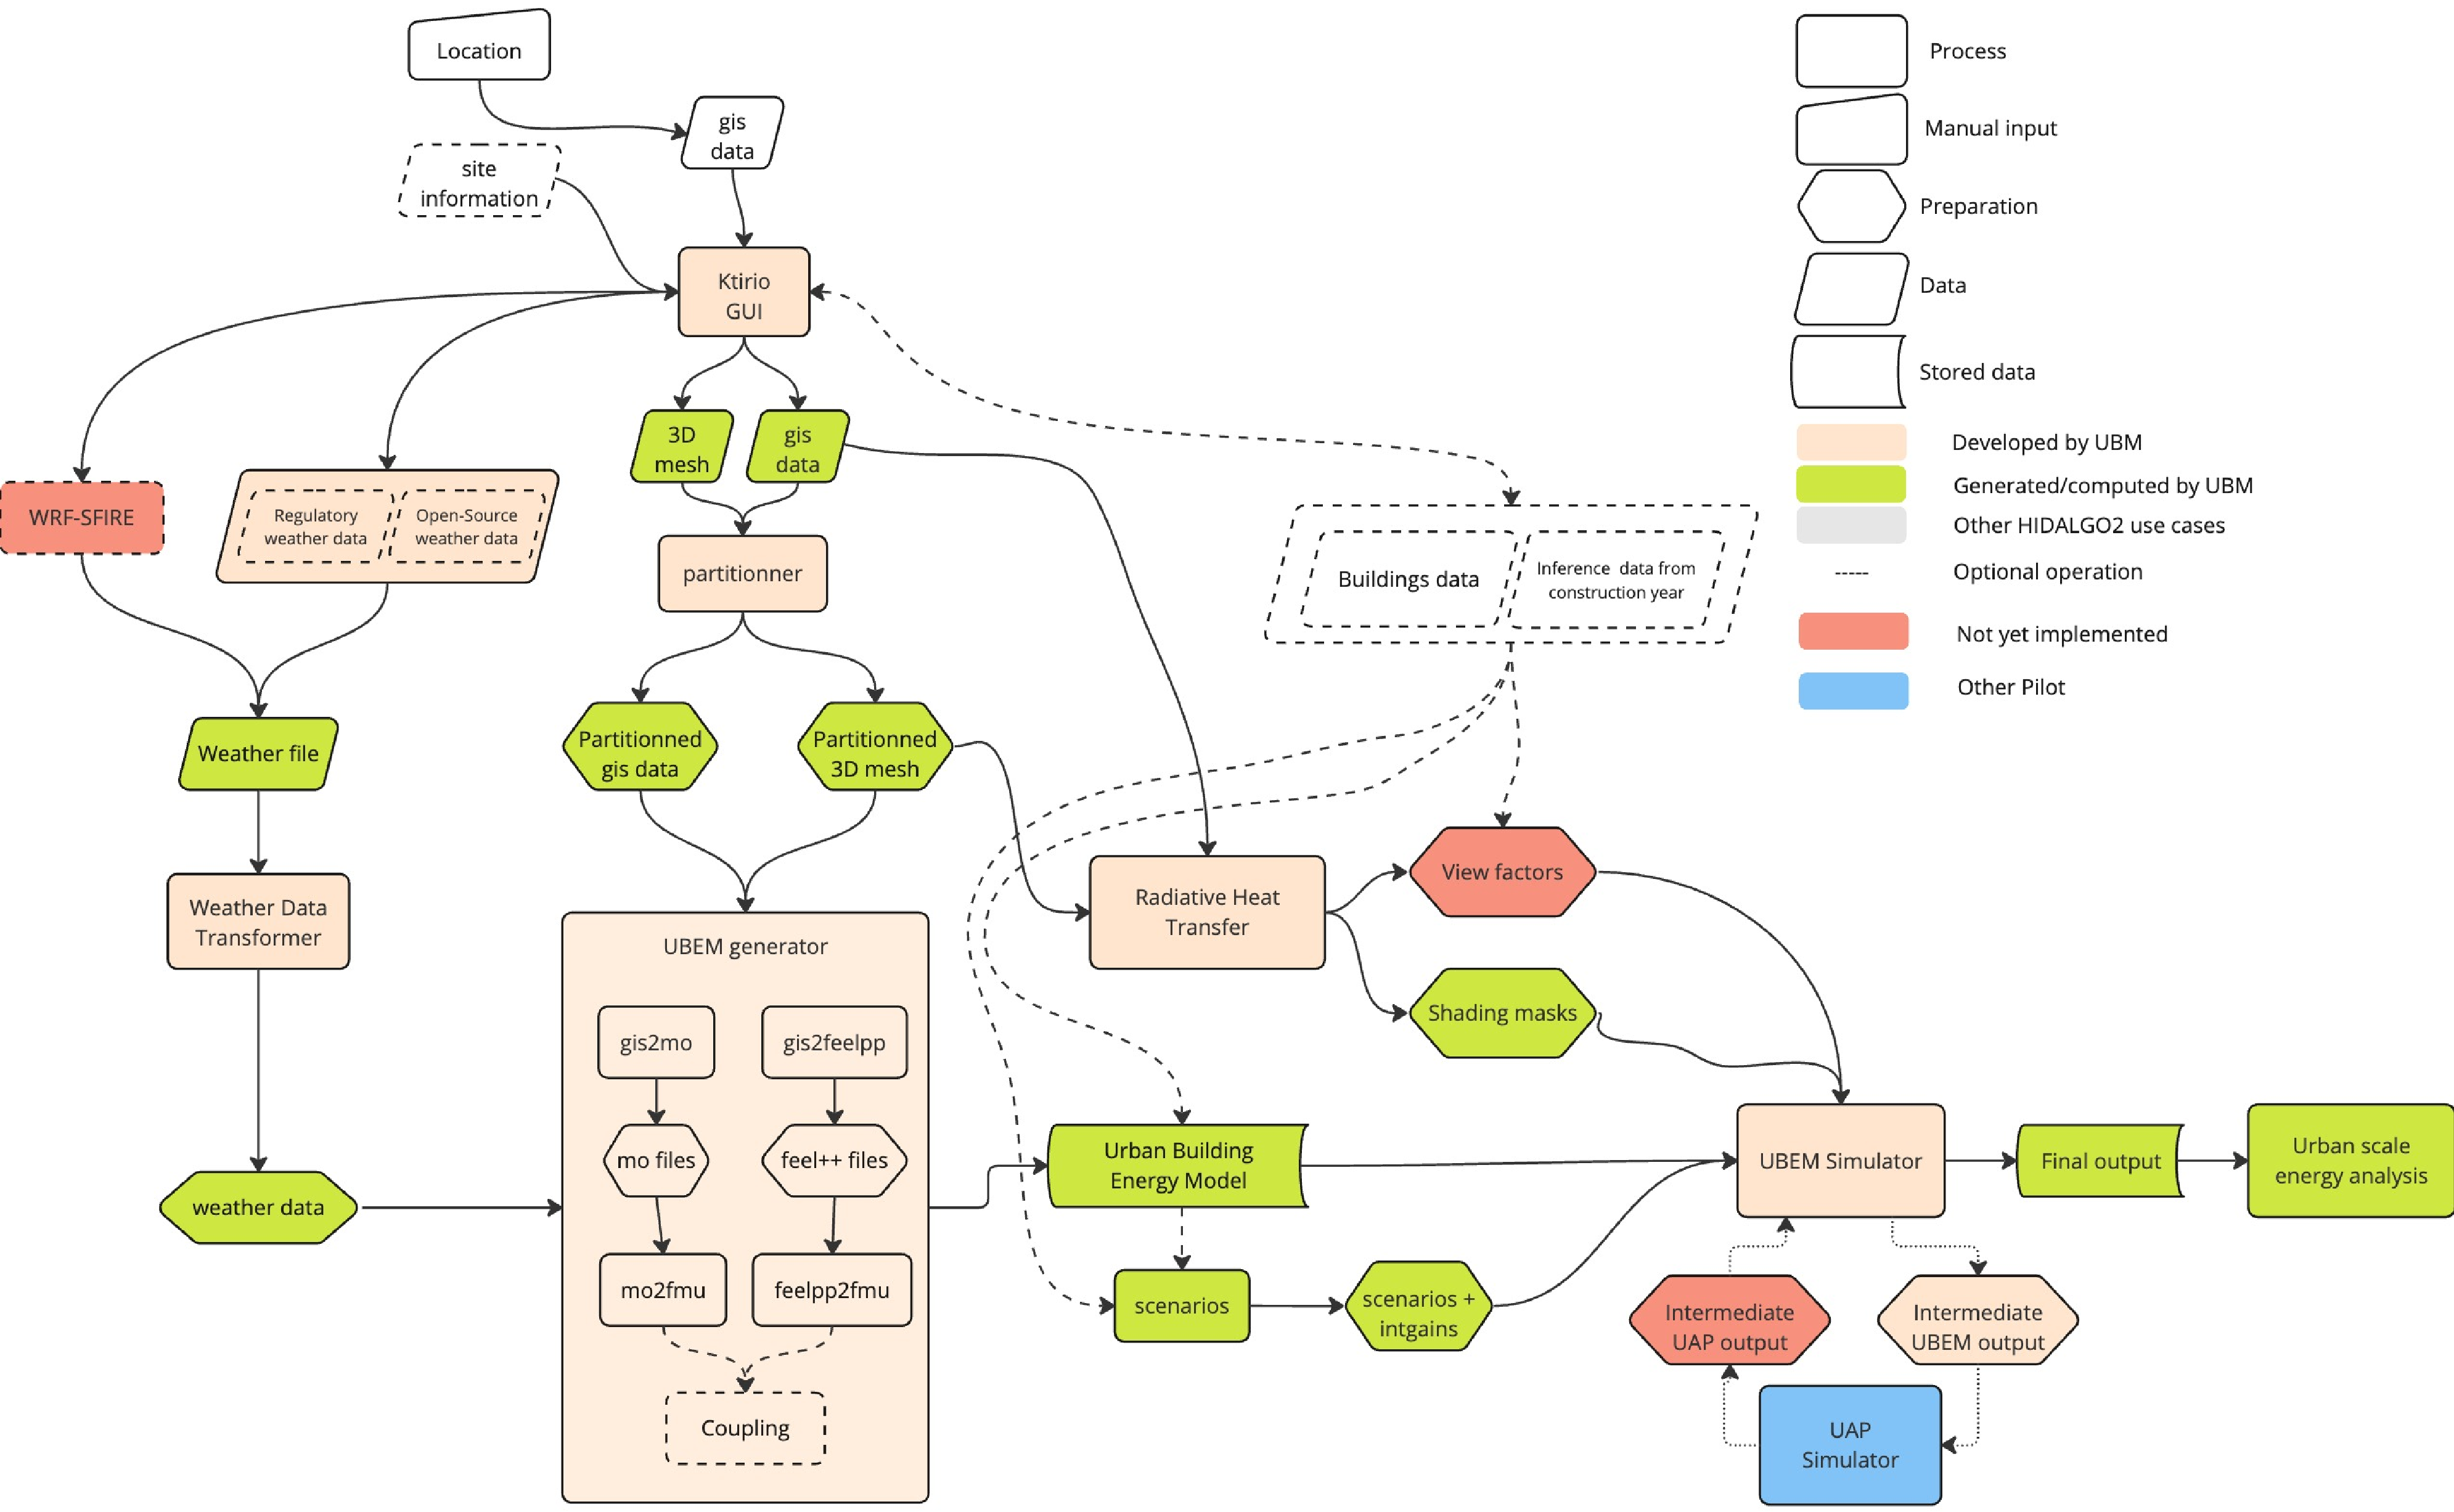
\includegraphics[width=.9\textwidth,page=1]{CP114_img-kub-workflow.pdf}
    \caption{Current Urban Building Workflow from localization to city energy simulation report.}
    \label{fig:kub-workflow}
\end{figure}


\subsection{Data Handling and Simulation Process}
\label{sec:data-handling}
\noindent
The workflow collects GIS and weather data, partitions them for scalable processing, and converts them via the \textit{UBEM Generator} into Modelica and Feel++~\cite{christophe_prudhomme_feelppfeelpp_2024} formats. 
The \textit{Urban Building Energy Model (UBEM)} then simulates energy usage and indoor conditions with a \textit{radiative heat transfer model}, computing \textit{view factors} and \textit{shading masks} that capture building-to-building interactions and contributions to the urban heat island effect. 
Finally, these building simulation outputs can drive the \textit{Urban Air Pollution (UAP) simulator} in a feedback loop, reflecting the interdependence of building energy consumption and urban air quality.
\subsection{Final Analysis and Urban Scale Energy Evaluation}
\label{sec:final-analysis}
\noindent
The final stage uses the \textit{UBEM Simulator} to produce large-scale outputs summarizing energy consumption and environmental impact at city scale, combining building energy and air quality data for a holistic perspective.

\noindent
To streamline data management, the simulator aggregates and exports key metrics (weather, energy, comfort) in JSON, then uploads them to a data platform via the CI/CD pipeline (\cref{fig:kub-devops}), which launches a reporting workflow as described in \cref{sec:cicd-framework}.

\noindent
Results are assembled into a report, automatically published on a website built with \textit{Antora}, allowing end users to explore outputs at both building and city levels.

\Cref{fig:ktirio-cases-report} presents a gallery of city reports that are taken as test cases for the Urban Building pilot, as well as an example of a city report section showing the occlusion factor and heat flow plot.
\begin{figure}[htbp]
  \centering
  \subfloat[Gallery of test case cities reports\label{fig:city-gallery}]{%
    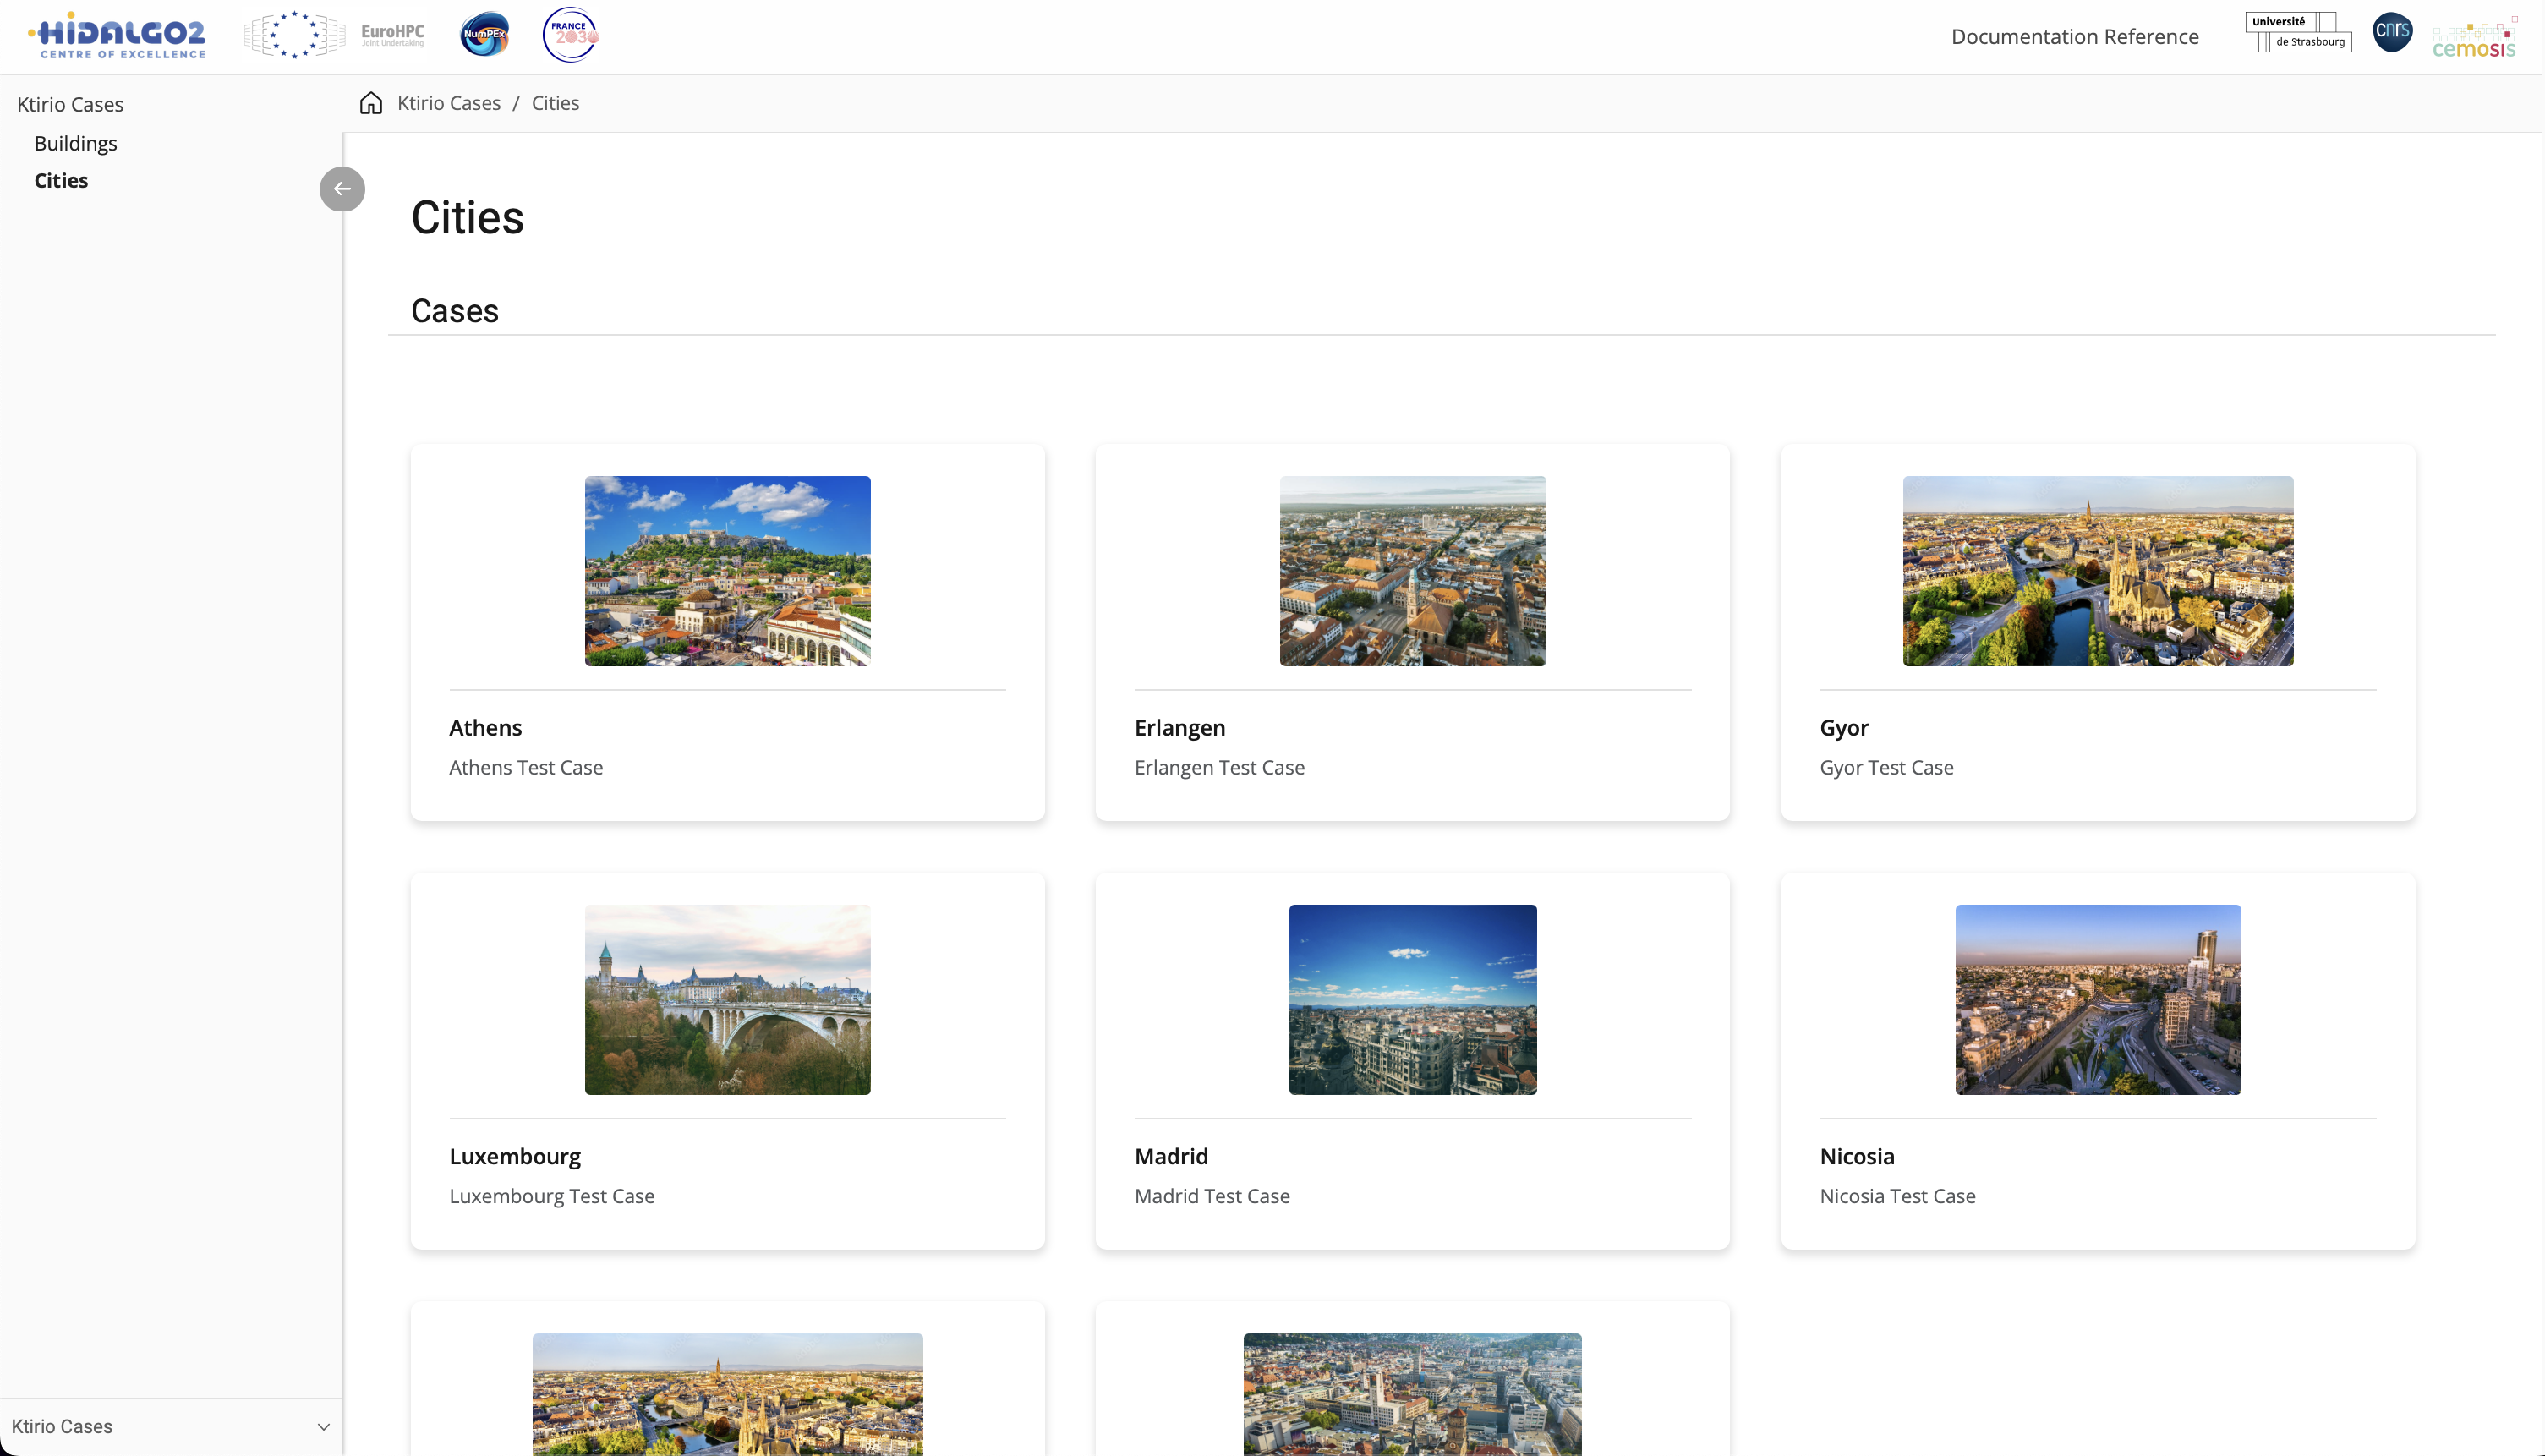
\includegraphics[width=0.45\textwidth]{CP114_img-city-gallery.png}
  }
  \hfill
  \subfloat[Section of a city report\label{fig:city-report-section}]{%
    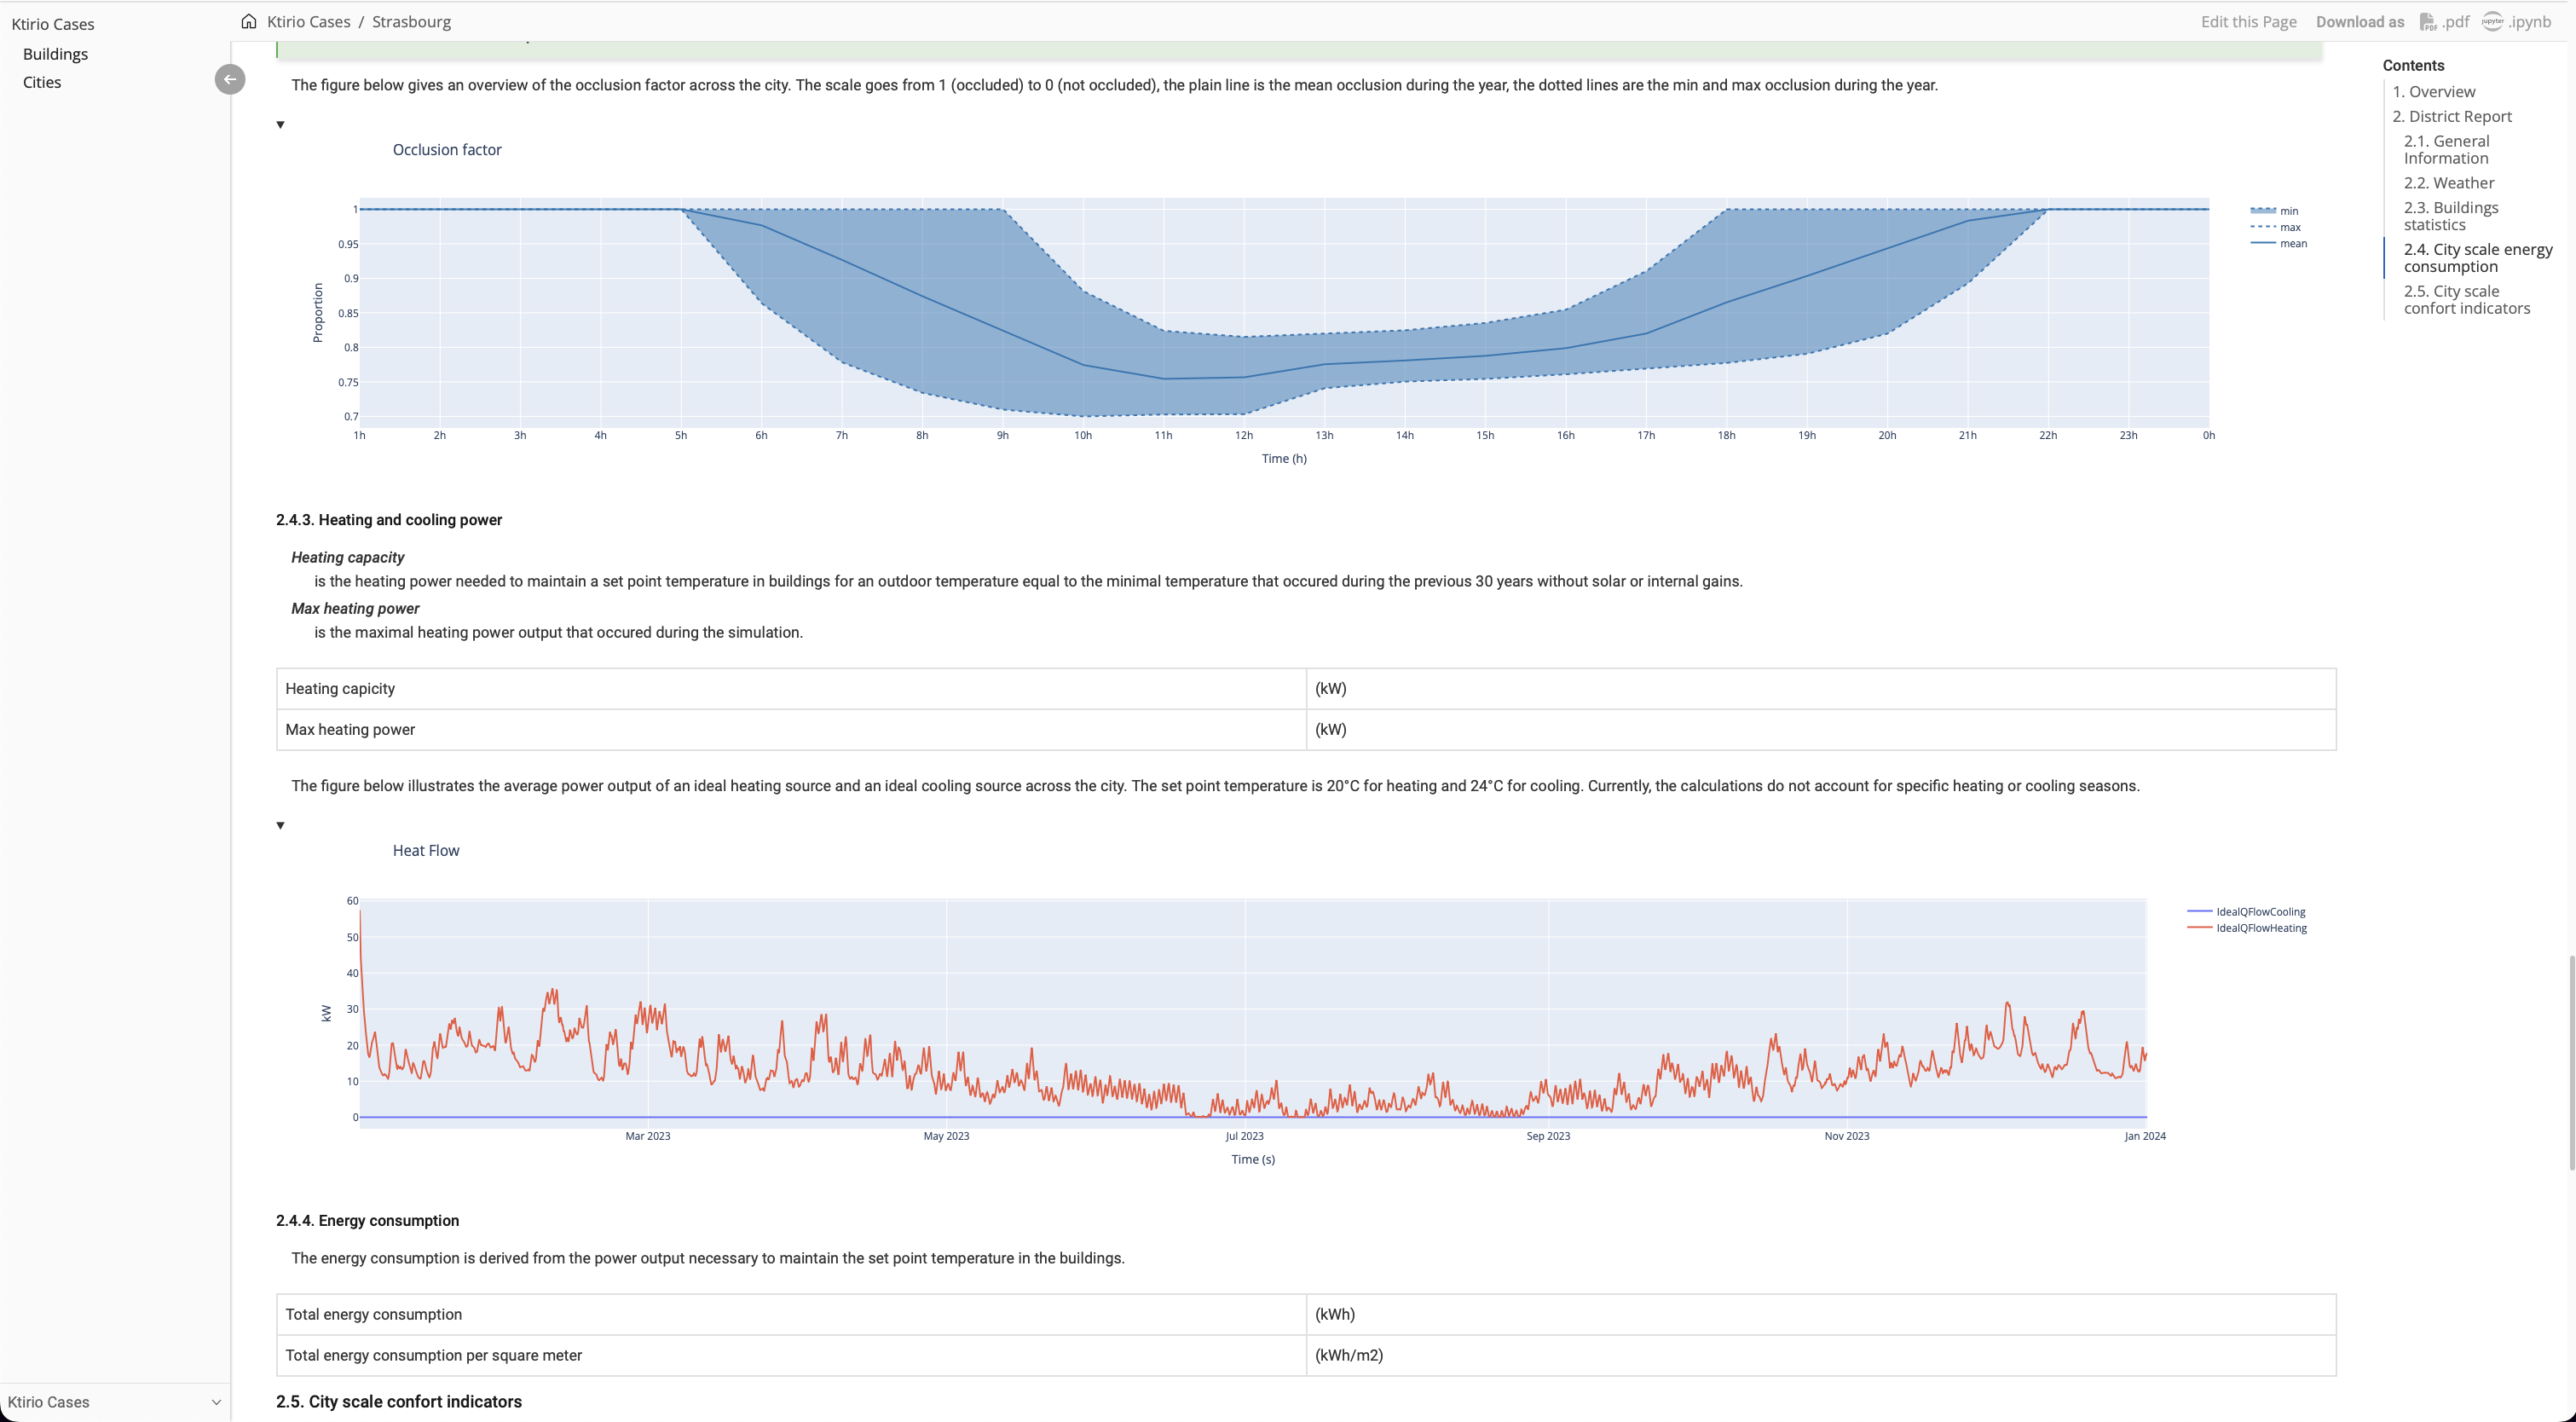
\includegraphics[width=0.45\textwidth]{CP114_img-city-report-section.png}
  }
  \caption{Screenshots of the \url{https://cases.ktirio.fr} reporting website.}
  \label{fig:ktirio-cases-report}
\end{figure}



\section{Overview of Urban Building Modeling and Simulation}
\label{sec:urban-building}

This section provides an overview of the geometrical and physical modeling and simulation components of our urban building application.

\subsection{Geometry Reconstruction of the KUB Urban Model}

\noindent
KUB's geometric reconstruction employs multi-fidelity approaches for buildings, terrain, vegetation, and roads. 
We use a tiled web map to manage data distribution and adapt the Level of Detail (LOD) as needed. 
\textbf{LOD-0} represents basic bounding boxes, \textbf{LOD-1} uses polygonal extrusions (including roof structures), and \textbf{LOD-2} integrates IFC-based standards with detailed geometry.

\noindent
\Cref{fig:buildings} illustrates these LODs: \Cref{fig:building-lod0} shows a bounding box (\textbf{LOD-0}), \Cref{fig:building-lod1} adds footprint extrusion (\textbf{LOD-1}), and \Cref{fig:building-lod2,fig:building-lod2-zoom} detail IFC-based BIM geometries (\textbf{LOD-2}). \Cref{fig:city-strasbourg} depicts Strasbourg's center, showcasing \textbf{LOD-0} (\cref{fig:city-strasbourg-lod0}) and \textbf{LOD-1} (\cref{fig:city-strasbourg-lod1}) representations.


\begin{figure}[ht]%{R}{1\textwidth} % 'R' or 'L' for right or left, and width
\centering
\subfloat[\textbf{LOD-0}: a building is represented by its bounding box]{%
  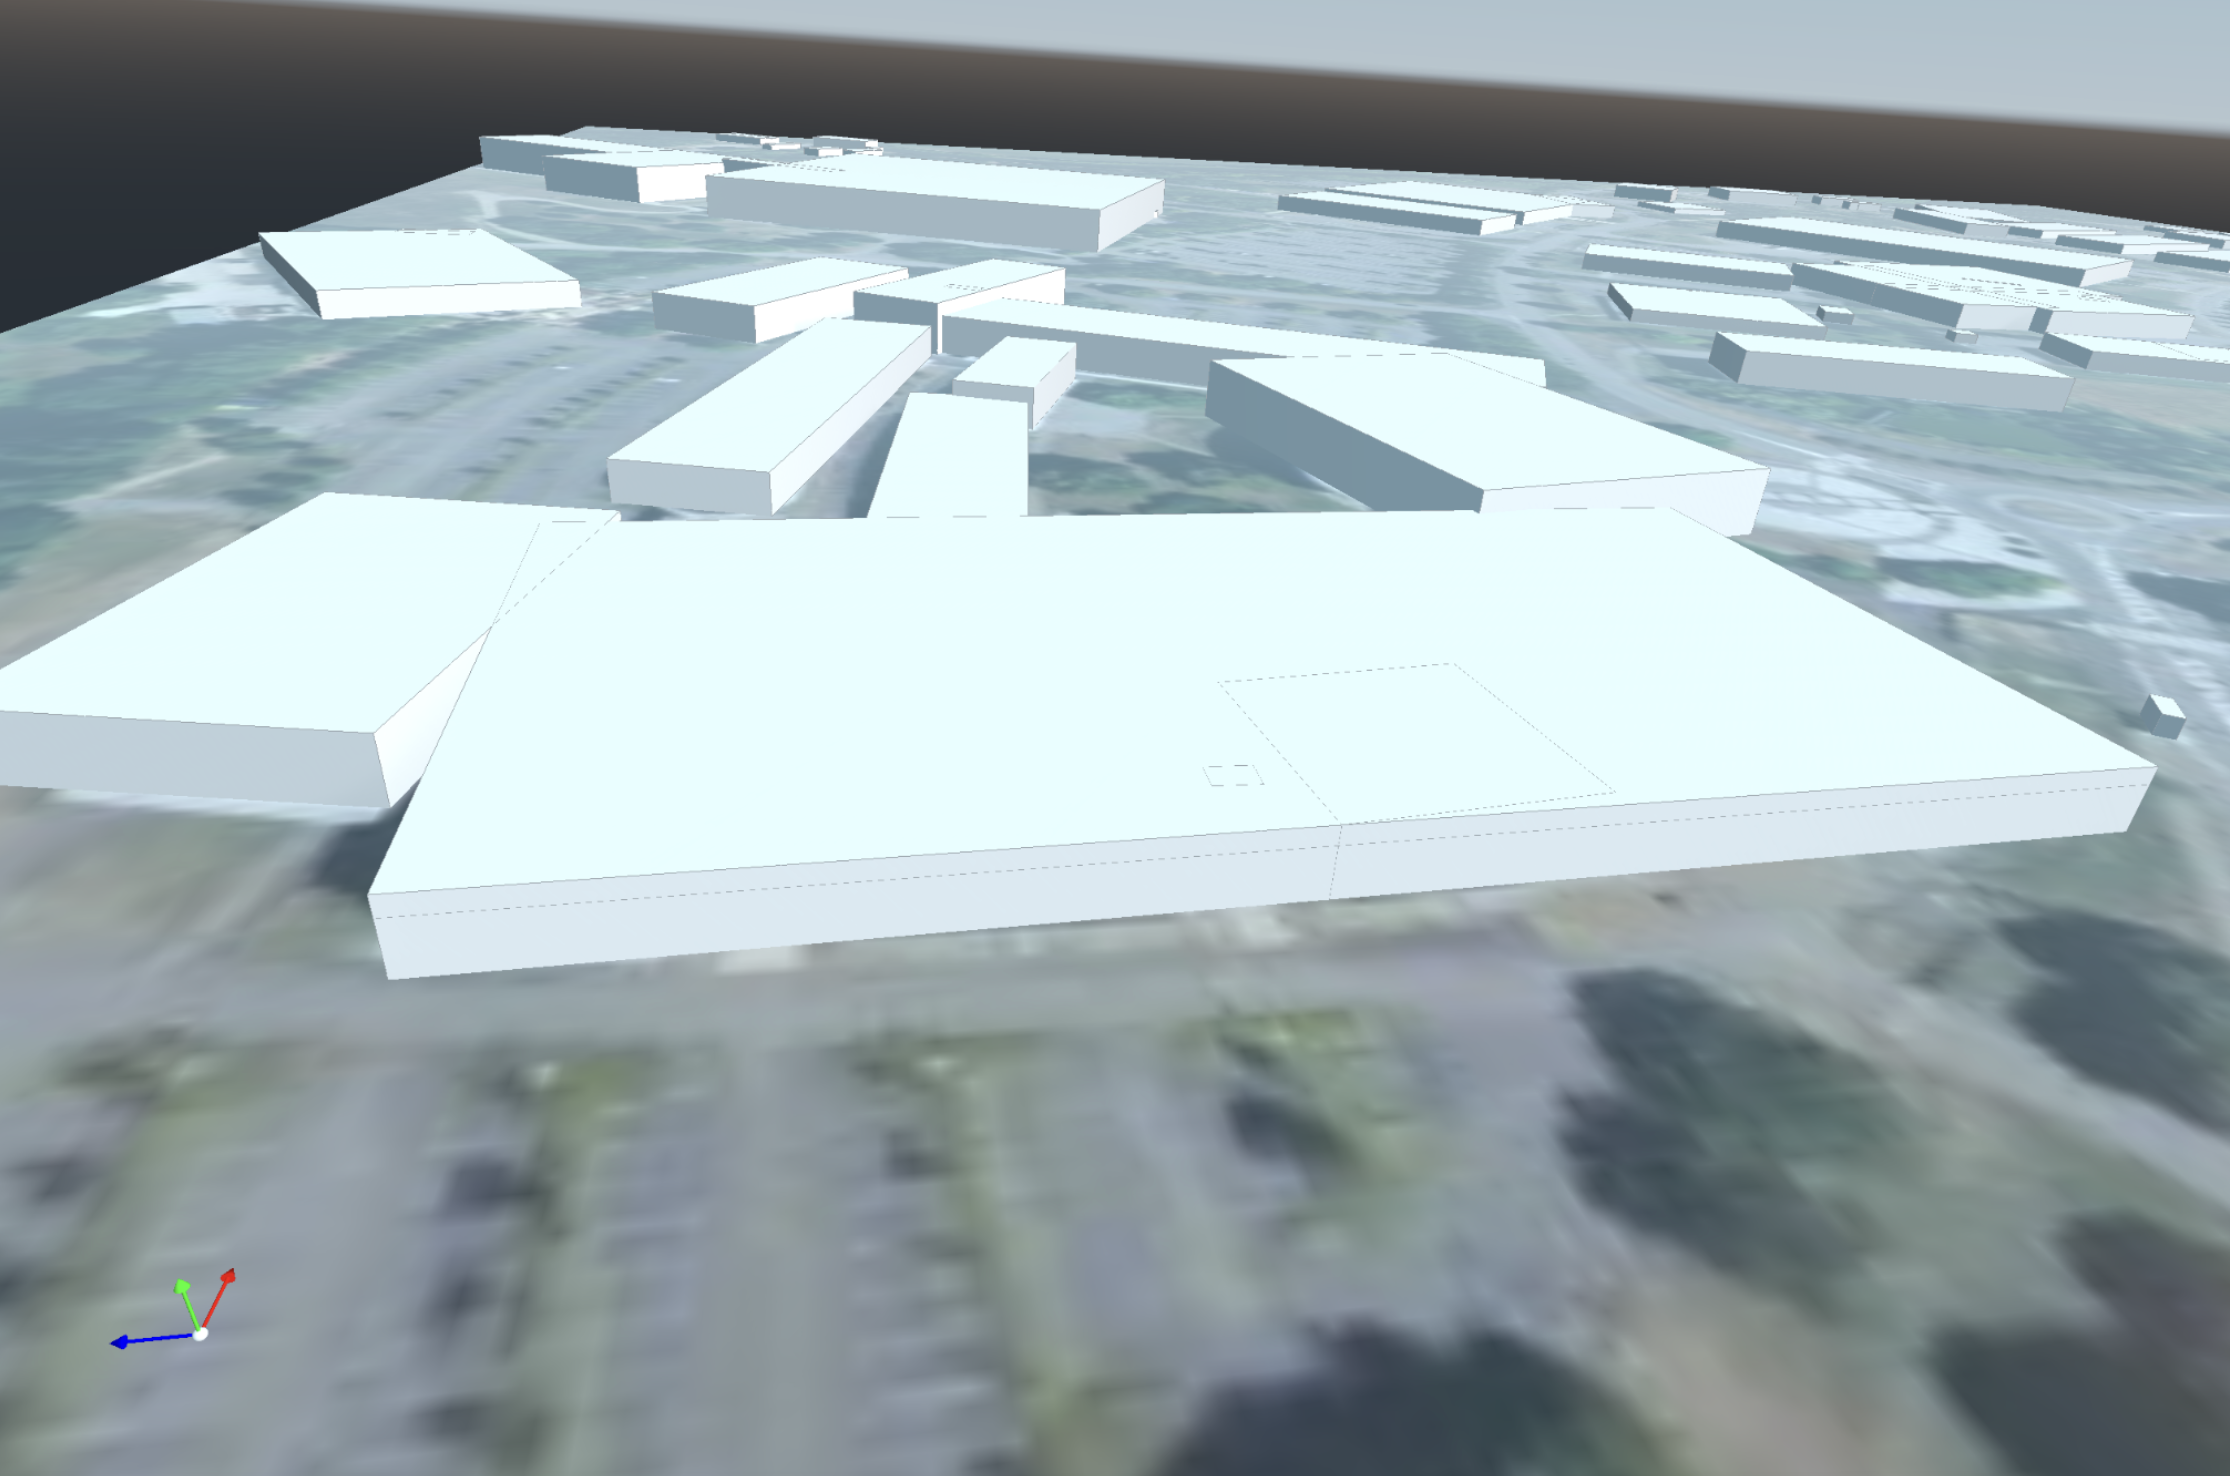
\includegraphics[width=0.45\linewidth]{CP114_img-buildings-lod0.png}
  \label{fig:building-lod0}
}\hspace{0.05\linewidth}
%\hfill % This ensures that the images are placed side by side
\subfloat[\textbf{LOD-1}: a building is represented by its ground footprint elevated to its height]{%
  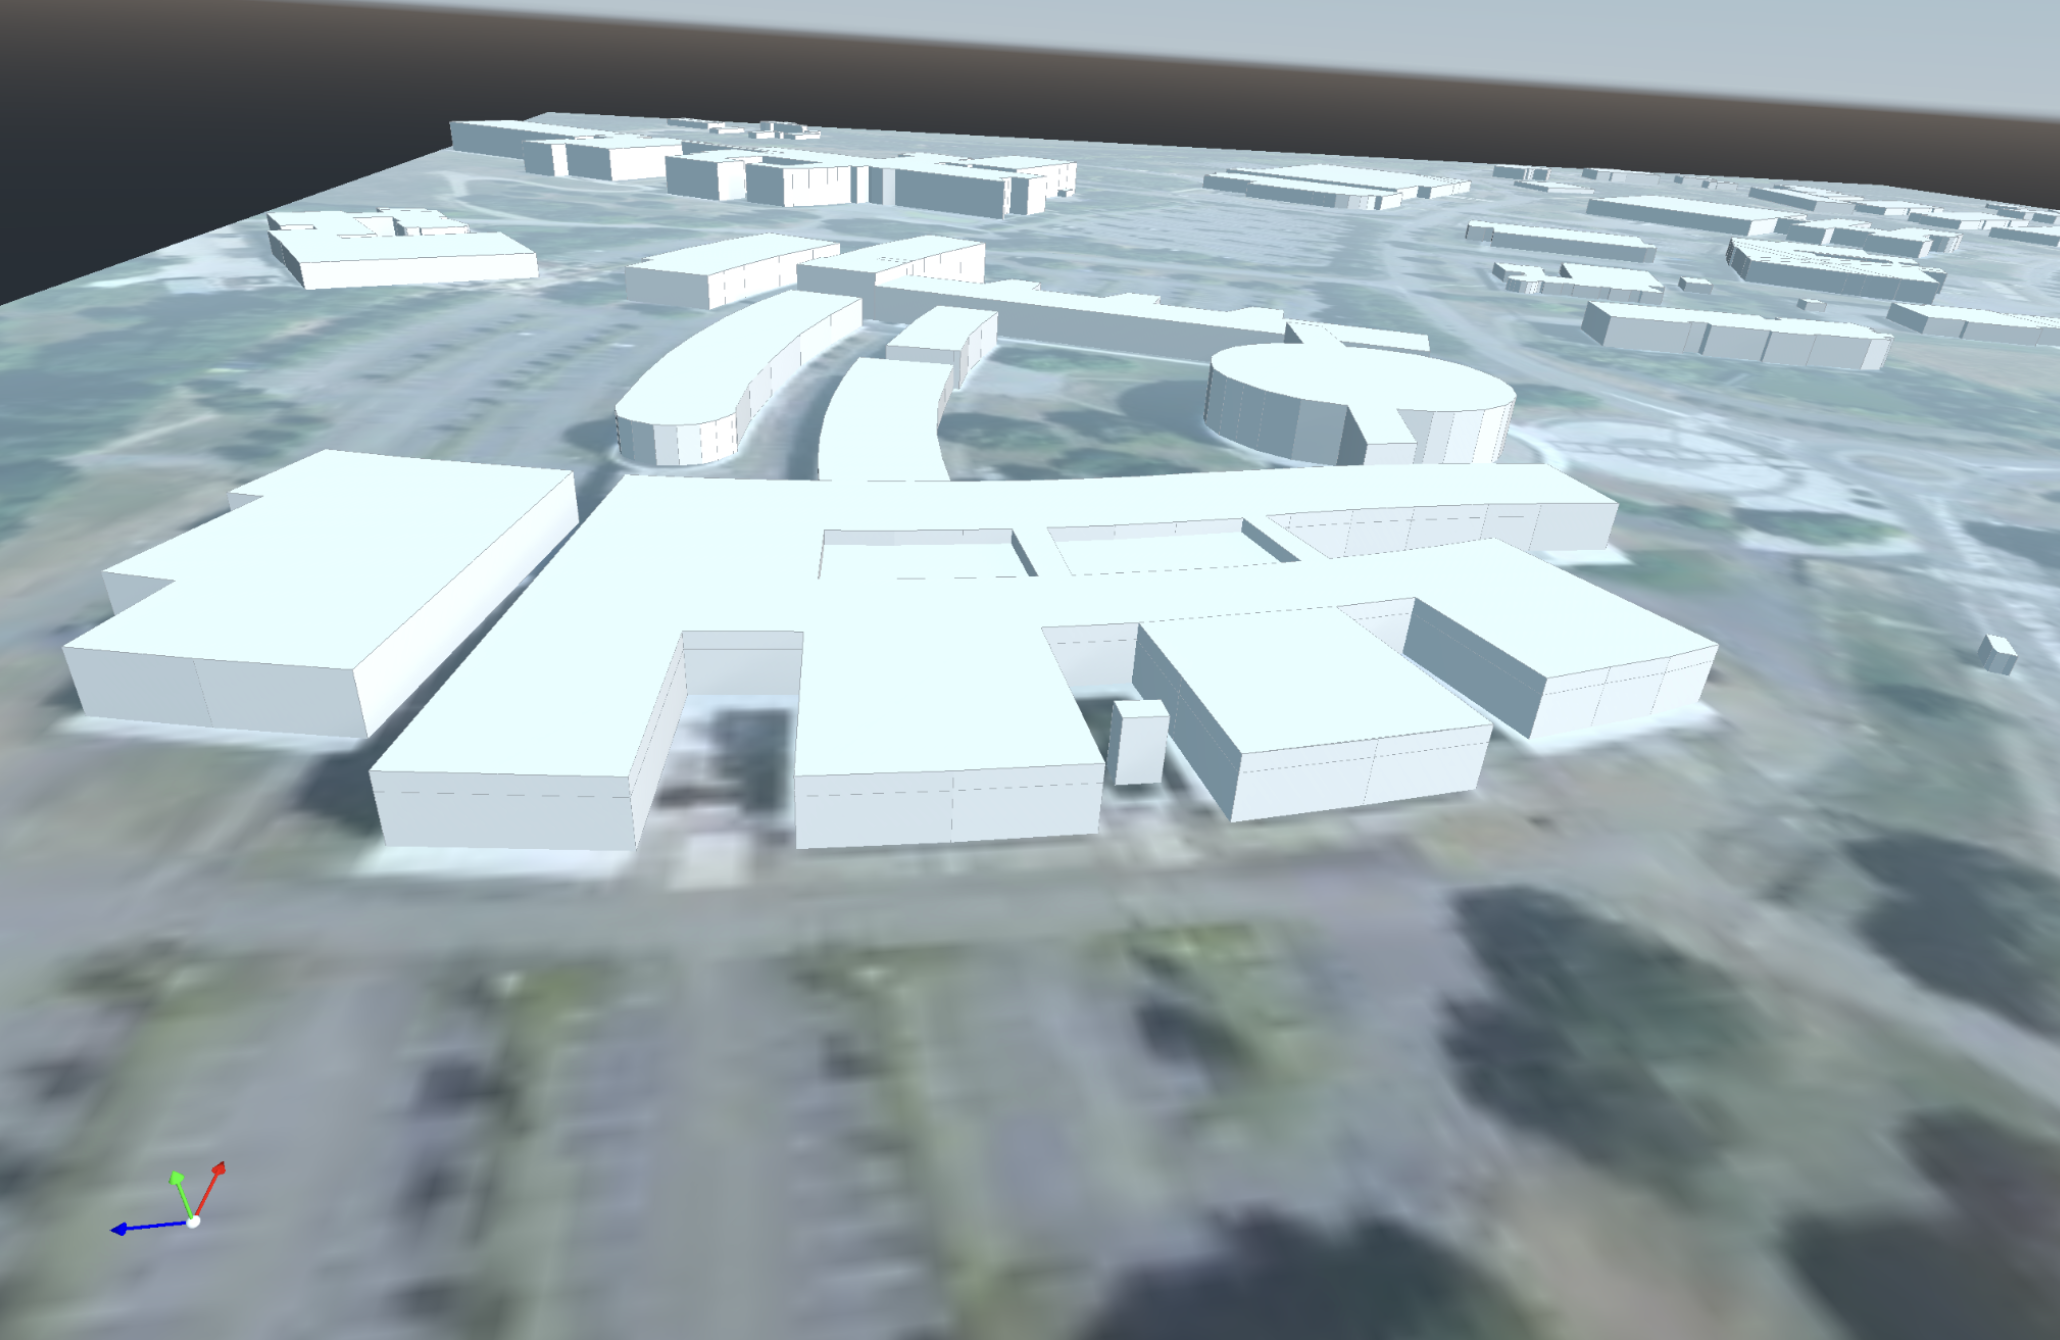
\includegraphics[width=0.45\linewidth]{CP114_img-buildings-lod1.png}
  \label{fig:building-lod1}
}\\ % Ends the line for the first row of figures

\subfloat[\textbf{LOD-2}: a building in full detail using BIM. Note that \textbf{LOD-2} and \textbf{LOD-1} are mixed.]{%
  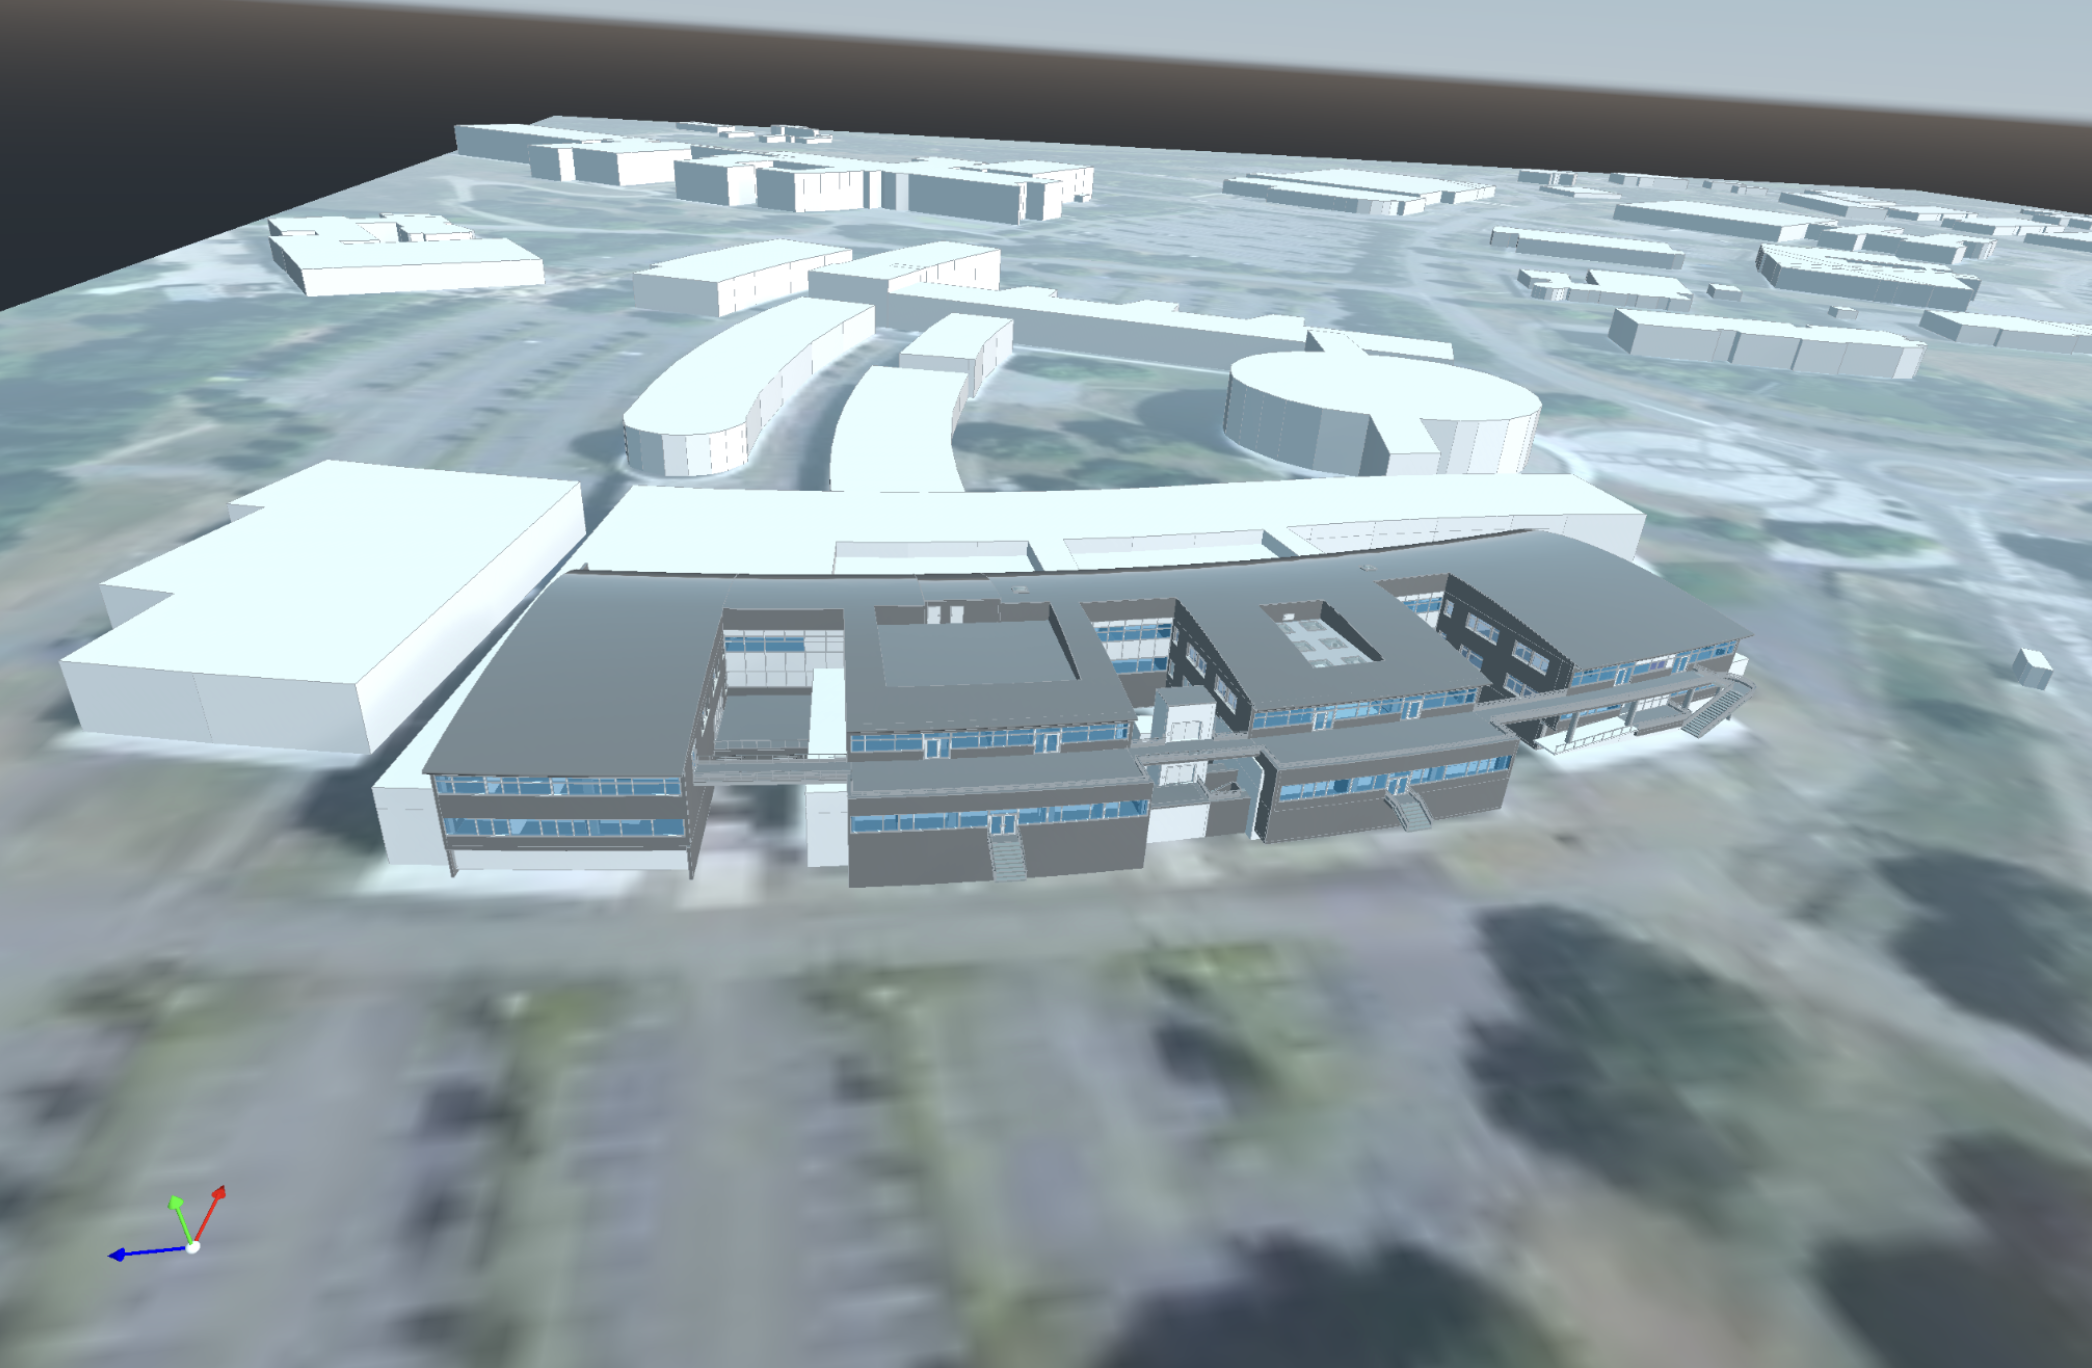
\includegraphics[width=0.45\linewidth]{CP114_img-buildings-lod2.png}
  \label{fig:building-lod2}
}\hspace{0.05\linewidth}
%\hfill
\subfloat[\textbf{LOD-2}: A zoom on the \textbf{LOD-2} building.]{%
  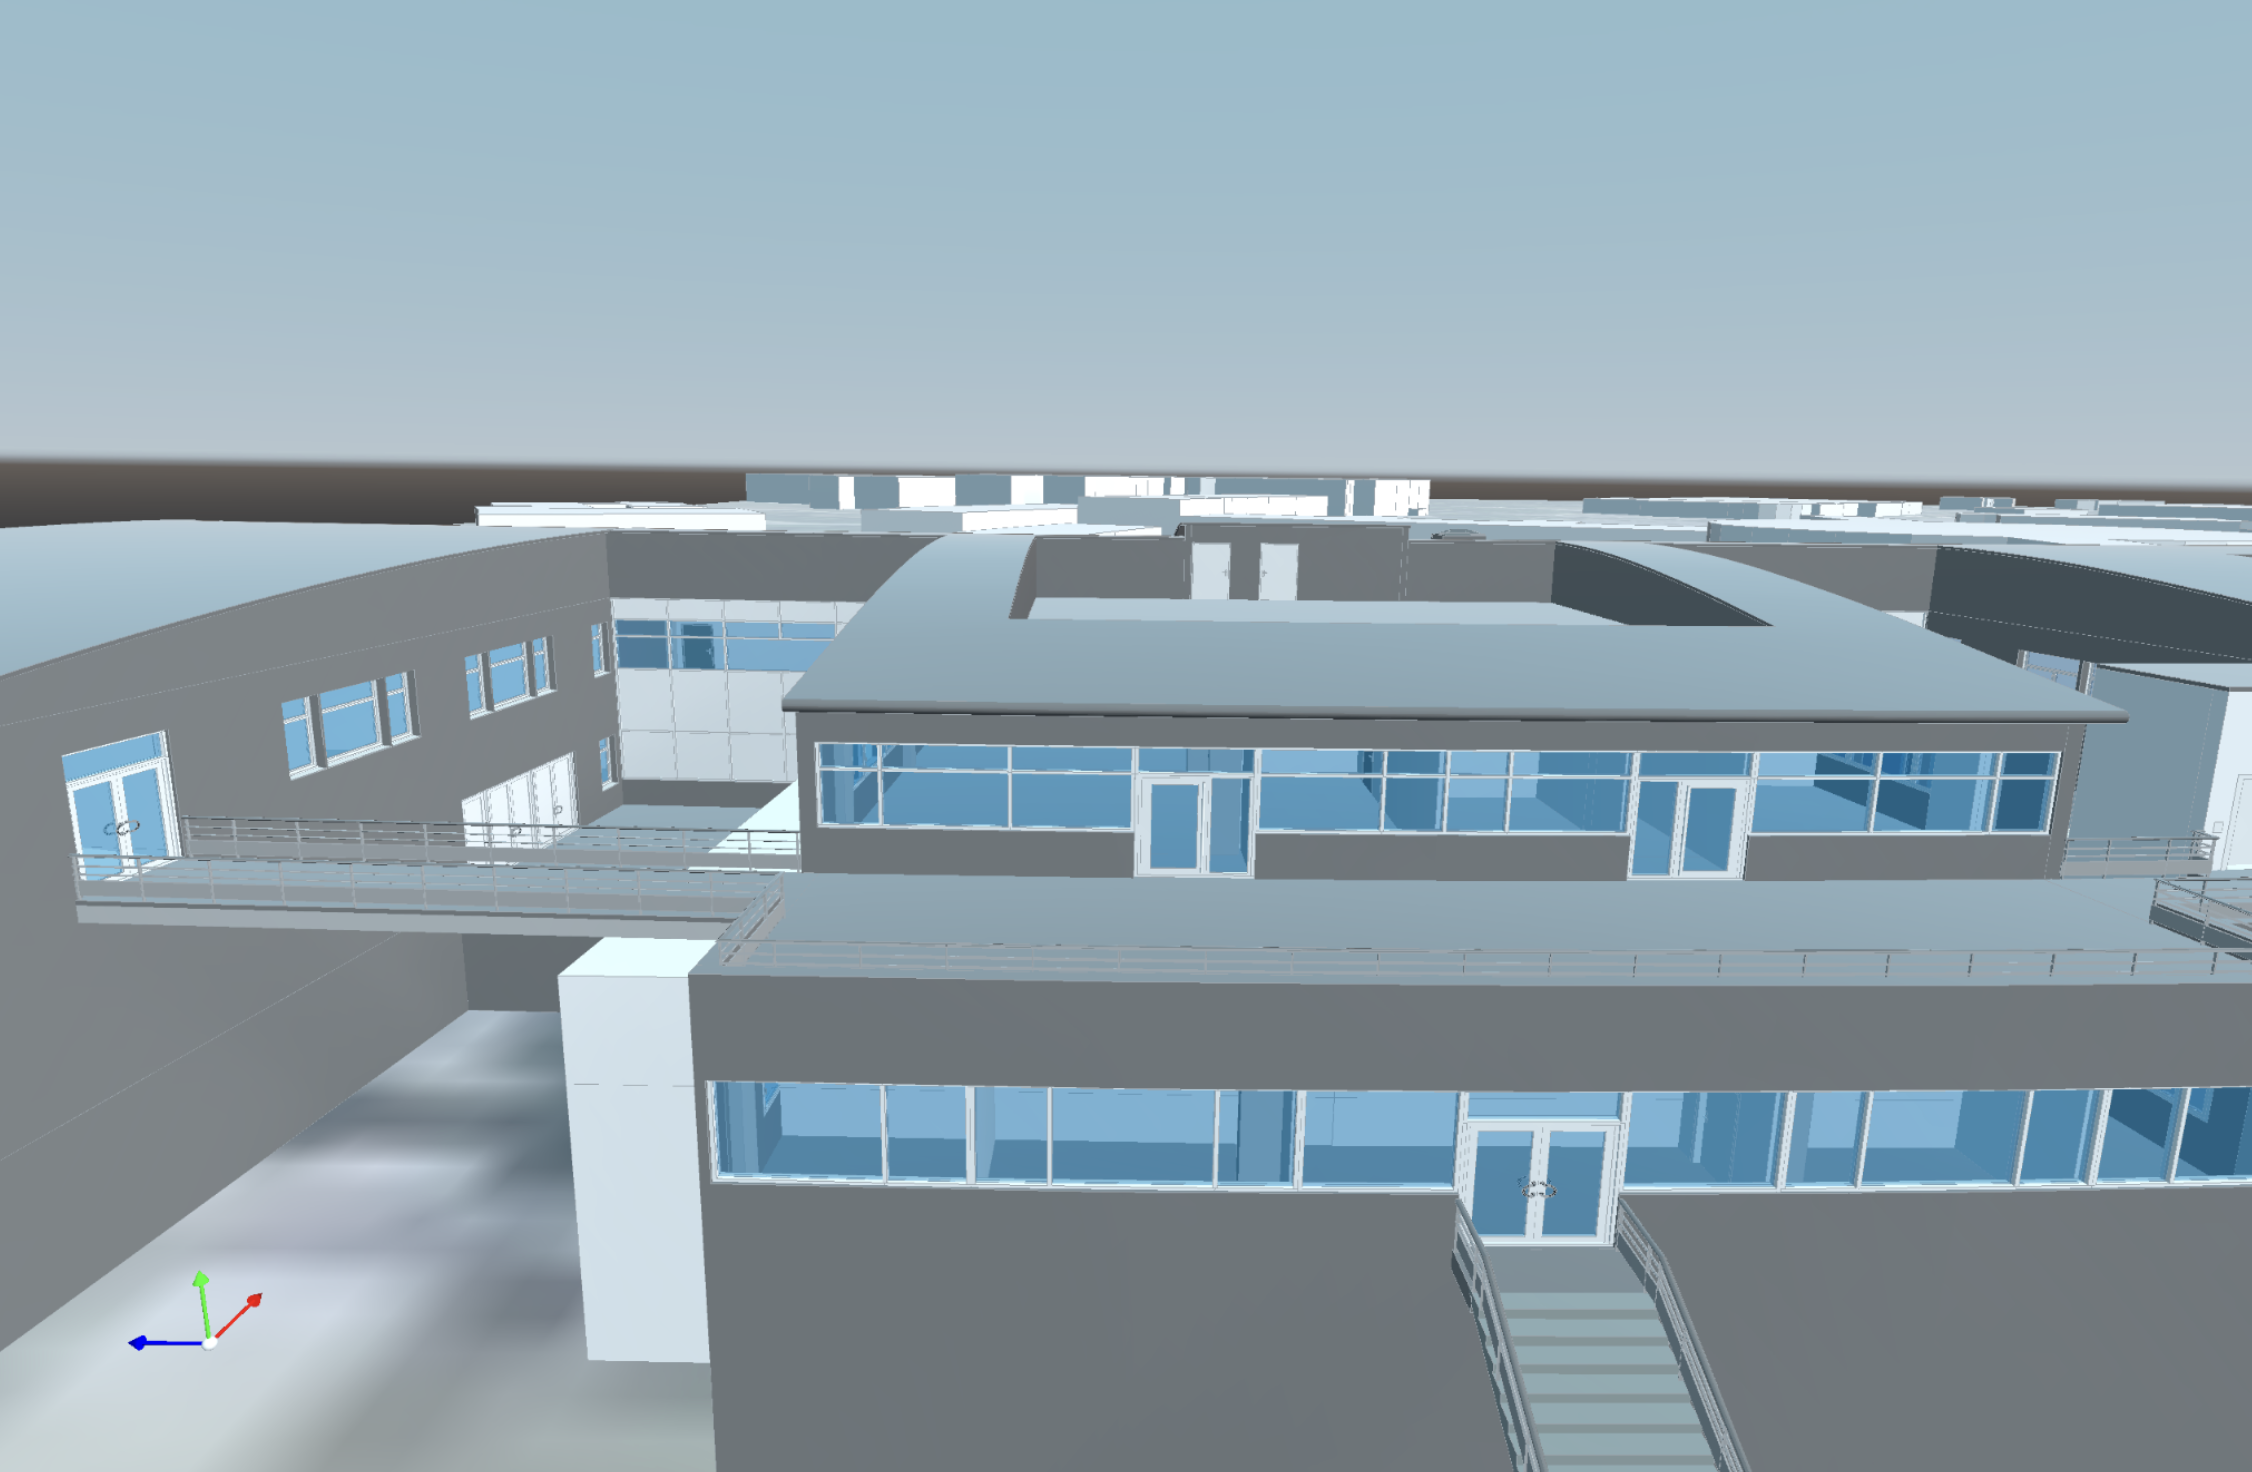
\includegraphics[width=0.45\linewidth]{CP114_img-buildings-lod2-zoom.png}
  \label{fig:building-lod2-zoom}
}

\caption{Different representations of a building using our LOD definition}
\label{fig:buildings}

\end{figure}




\subsubsection{Building Modeling}

Building meshes are generated from OpenStreetMap data~\cite{openstreetmap_contributors_planet_2017}, which provides multi-polygons with holes. For \textbf{LOD-0 and LOD-1}, 2D footprints are extruded to form 3D volumes, merging or subtracting intersecting buildings to create district-scale models. In \textbf{LOD-2}, conformal watertight meshes are produced from BIM data in IFC format, supporting detailed simulations of building components.

\subsubsection{Terrain Modeling}
Terrain is derived from elevation raster data, generating a uniform mesh sized to the raster. Each node's elevation is then evaluated. To avoid over-refinement, we plan a mesh adaptation approach \begin{inparaenum}[\it (i)]\item computing multiple elevation isolines, and \item building a mesh conforming to these isolines\end{inparaenum}.

\subsubsection{Vegetation Modeling}
Vegetation data (trees) from OpenStreetMap supplies positions, heights, and species. We maintain a reference library of tree geometries at various LODs, applying affine transformations as follows: \begin{inparaenum}[\it (i)]\item define a tree library, \item fetch metadata (height/species), and \item build a geometric model based on the library\end{inparaenum}. This accounts for shading and cooling effects in building environments.

\subsubsection{Integration of all urban geometric components}

We construct a conforming mesh that merges buildings, terrain, and vegetation. Key tasks are: \textit{(i)} adapting building heights to slopes and embedding them into the terrain (\cref{fig:city-grenoble-terrain}); \textit{(ii)} intersecting buildings to define contact zones for thermal coupling; \textit{(iii)} intersecting vegetation with buildings and terrain; and \textit{(iv)} refining the mesh after these geometric operations.


\subsubsection{Visual Representation}
Advanced rendering techniques visualize these multi-fidelity urban models for detailed analyses and broader urban planning discussions. Such visualizations help assess potential impacts of urban developments and engage diverse stakeholders.

This methodology offers enhanced precision, utility, and scalability, making it integral to the HiDALGO2 project's urban analysis and planning activities.

%\begin{wrapfigure}{R}{0.6\textwidth}
\begin{figure}[ht]
\centering
\subfloat[Representation of Strasbourg center with LOD-0\label{fig:city-strasbourg-lod0}]{%
  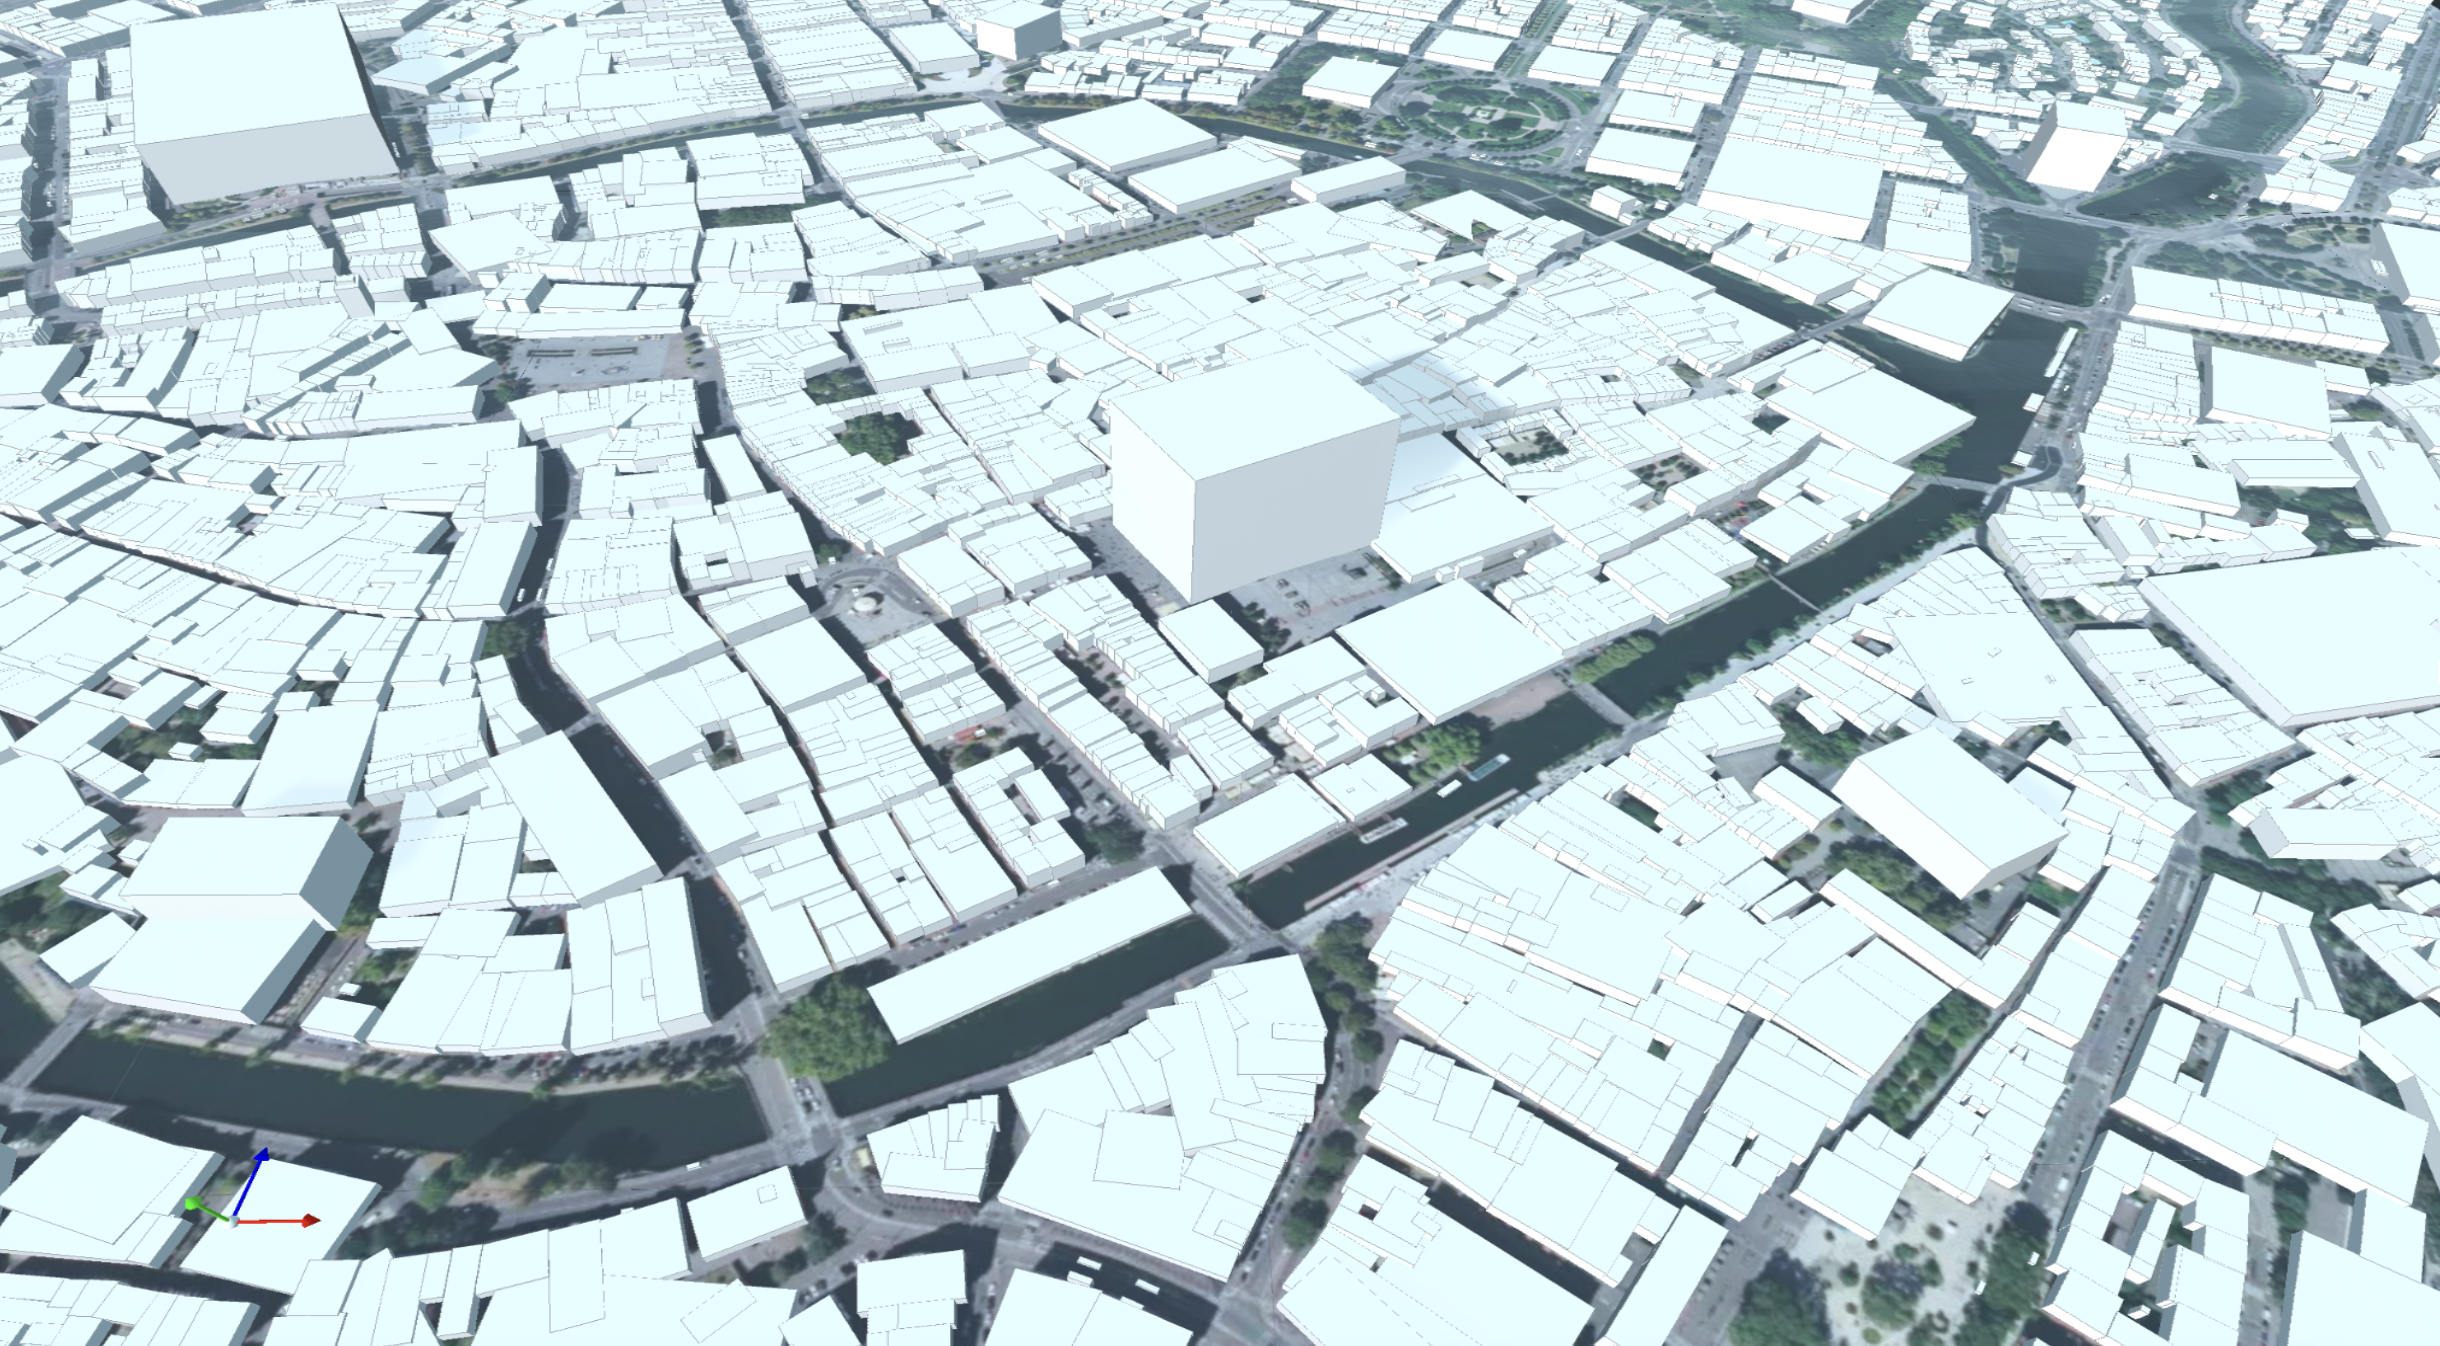
\includegraphics[width=0.48\textwidth]{CP114_img-city-strasbourg-lod-0.png}
}
\hfill % Ensures that the images are placed side by side
\subfloat[Representation of Strasbourg center with LOD-1\label{fig:city-strasbourg-lod1}]{%
  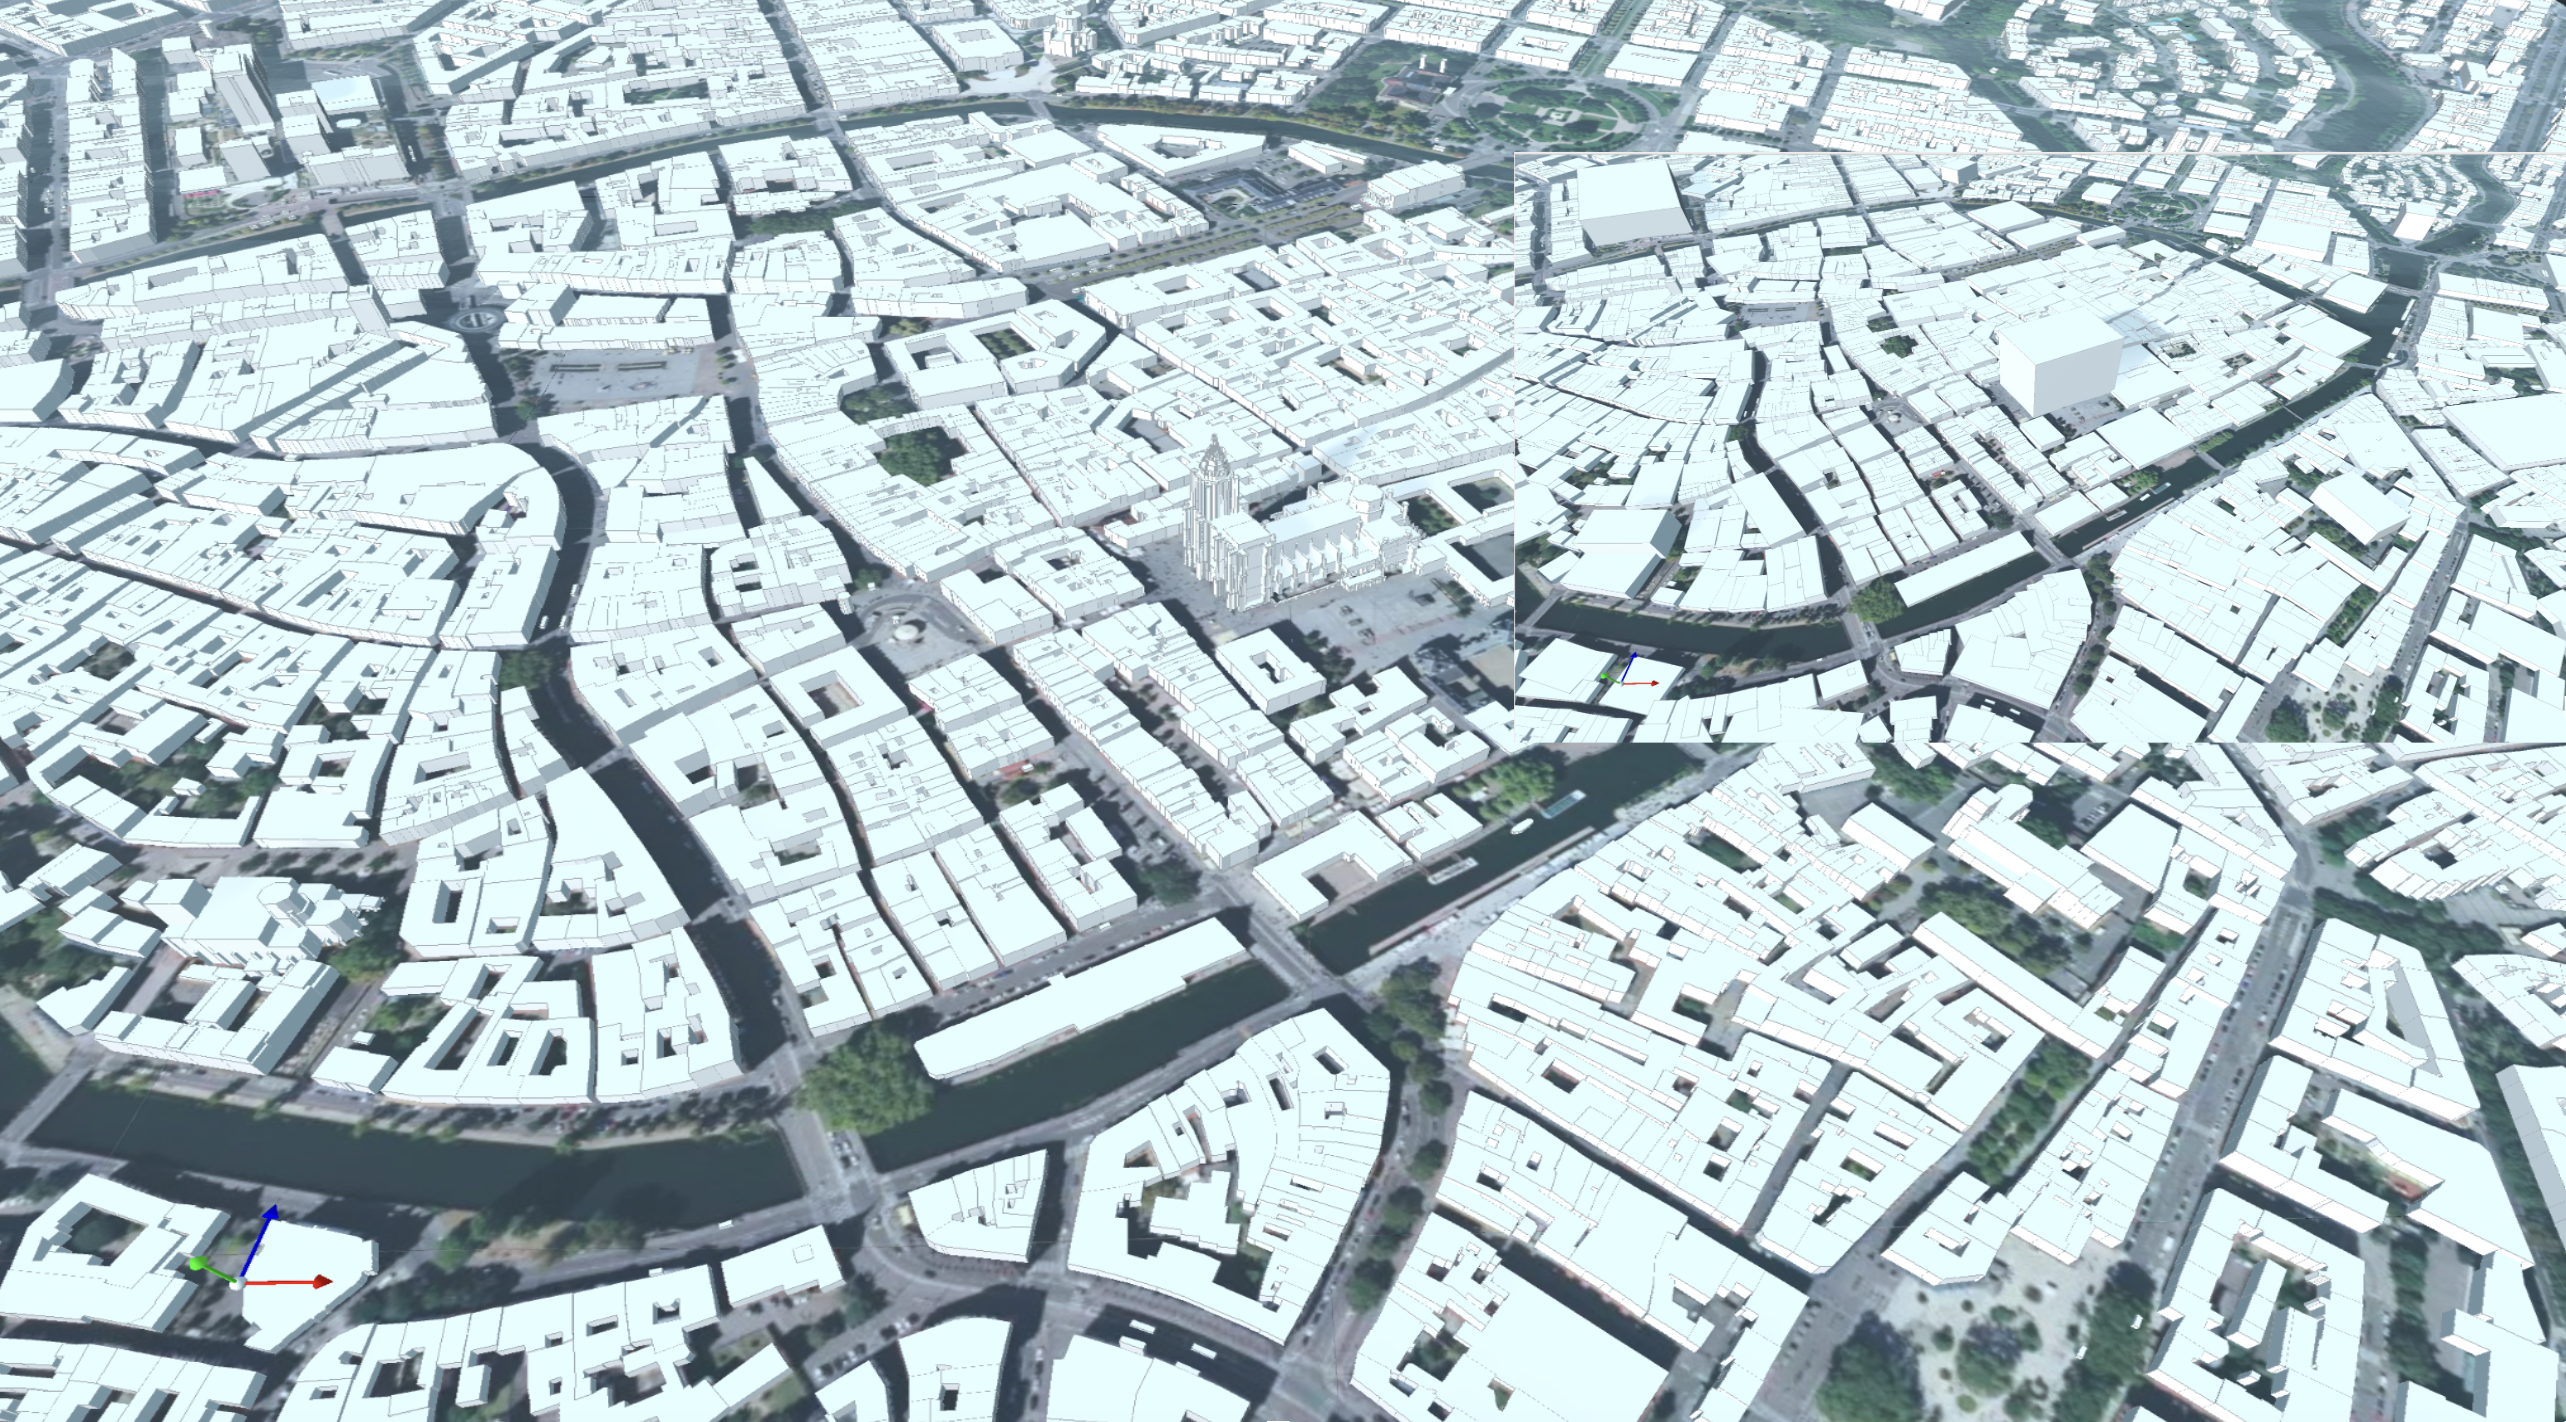
\includegraphics[width=0.48\textwidth]{CP114_img-city-strasbourg-lod-1.png}
}\\ % Ends the line for the first row of figures

\subfloat[Representation of Grenoble LOD-1 terrain elevation\label{fig:city-grenoble-terrain}]{%
  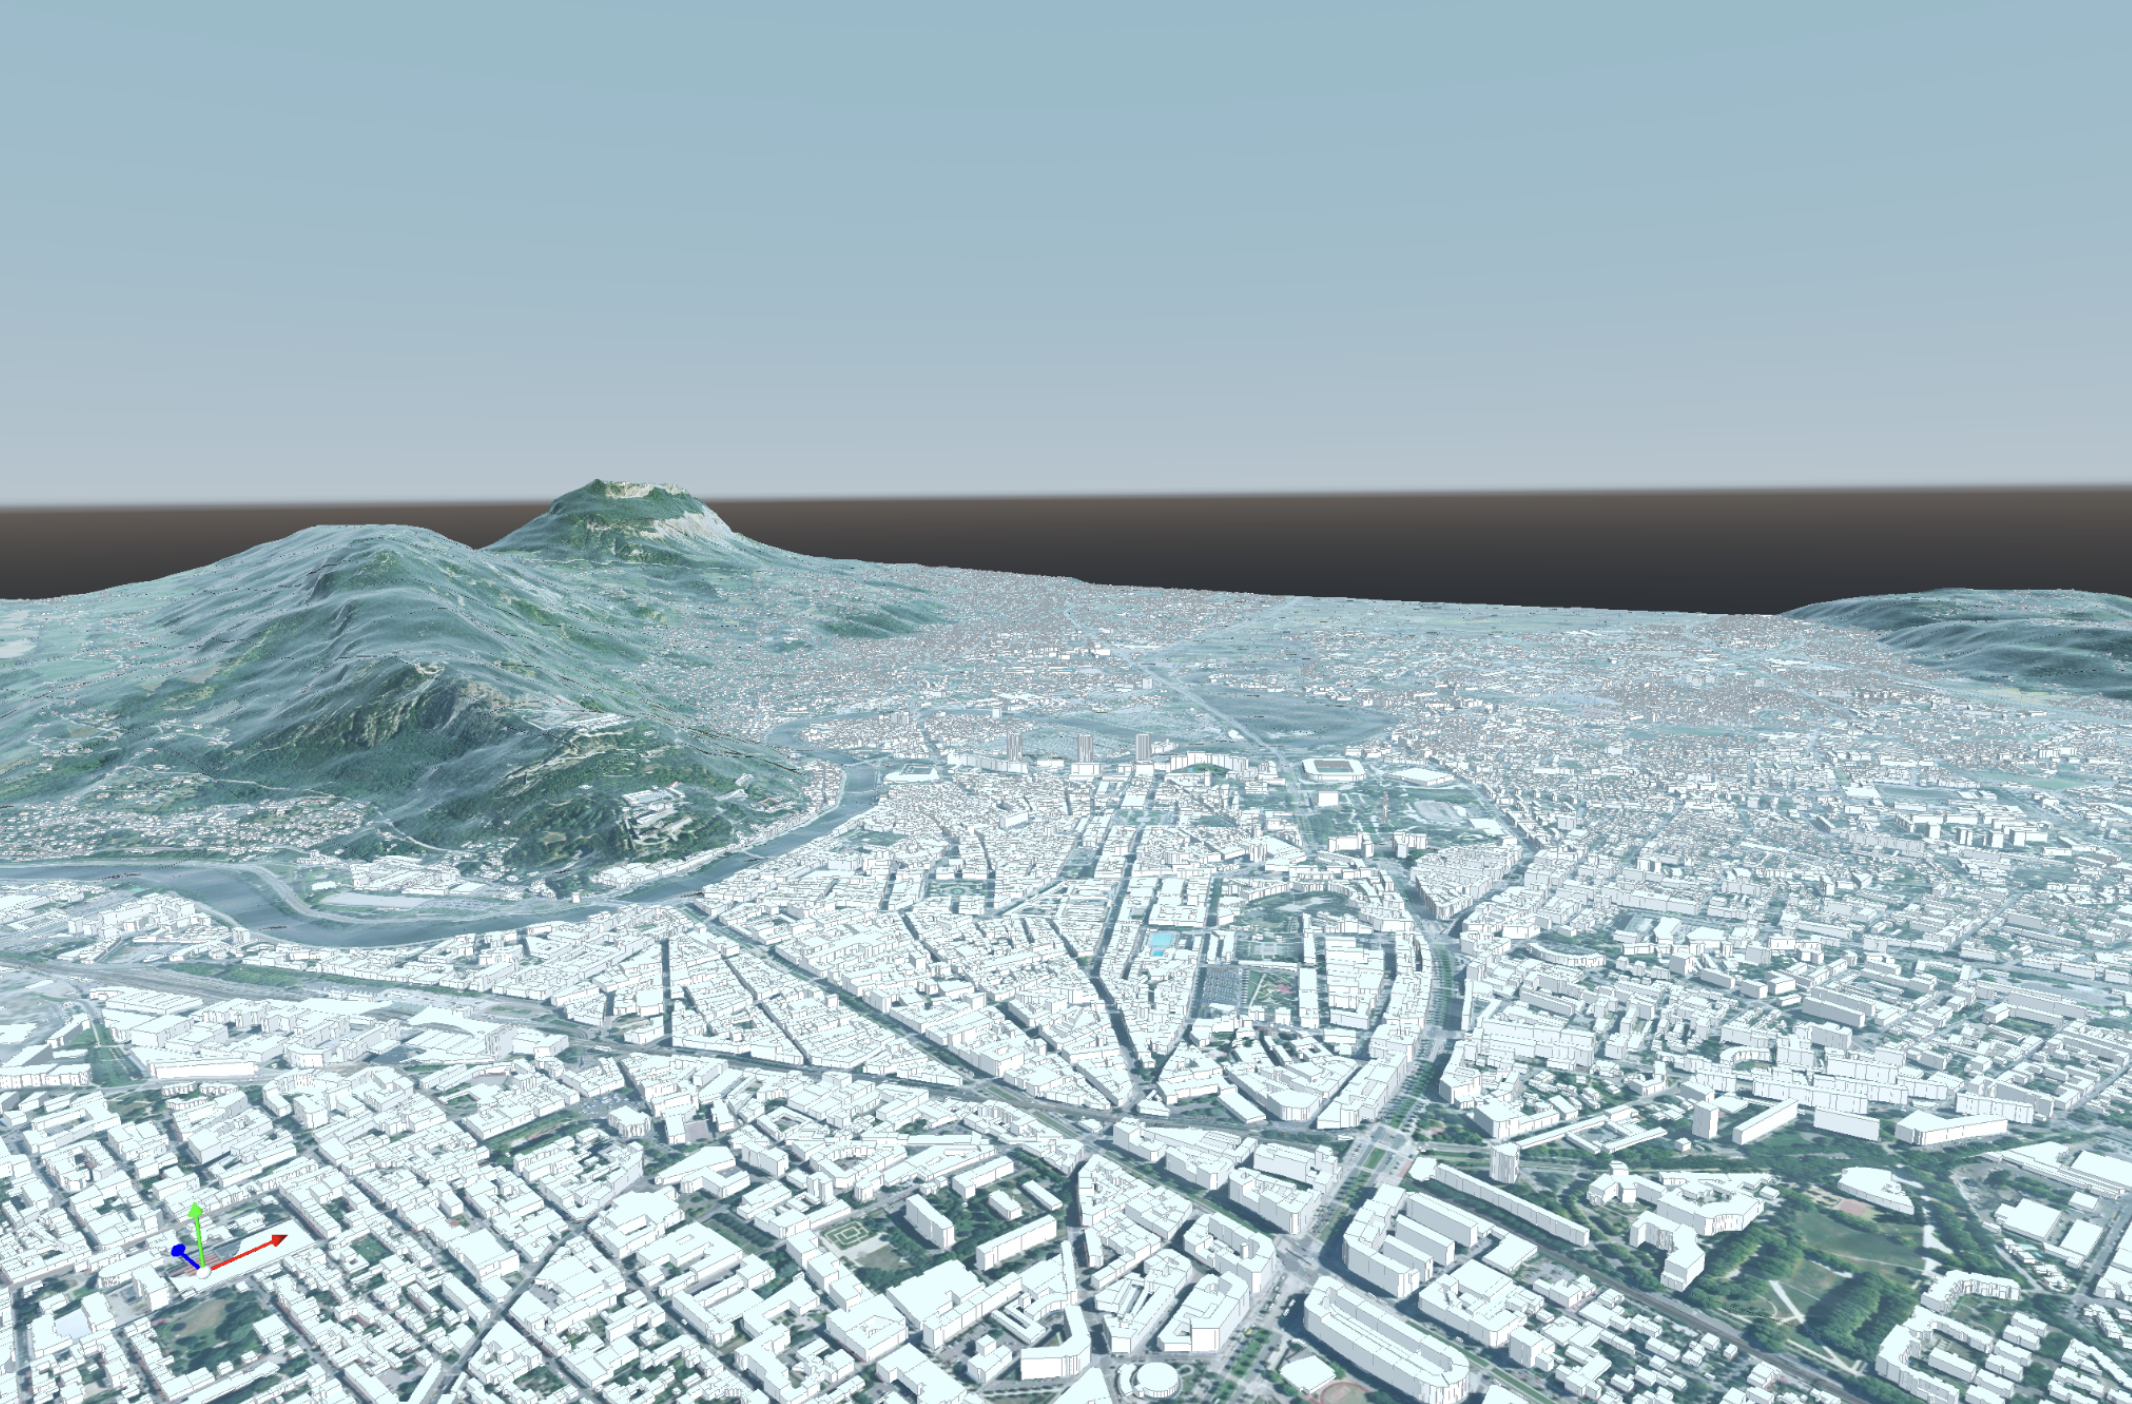
\includegraphics[width=0.48\textwidth]{CP114_img-city-grenoble-terrain.png}
}

\caption{Various representations of cities and terrains}
\label{fig:city-strasbourg}
%\vspace{-0.5cm}
\end{figure}
%\end{wrapfigure}

\subsubsection{Computational Tools for Mesh Generation}

In our urban modeling, CGAL~\cite{the_cgal_project_cgal_2024} tackles complex geometric tasks such as boolean operations, multi-polygon repairs~\cite{loriot_polygon_2024}, mesh generation, mesh intersection, and roof skeleton computation. 
We can already reconstruct a geometric model for any selected location, assembling LOD-0 or LOD-1 buildings with terrain elevation. The integration of all urban components remains under development, since mesh intersection algorithms are computationally expensive and require strategic grouping to reduce costs.

\paragraph{Current Mesh Generation Strategy}
We leverage multi-threading (MT) to download GIS data and repair polygons~\cite{loriot_polygon_2024} in parallel, then generate terrain meshes using CGAL. Union operations at tile edges run sequentially, while building meshes are created in parallel.

\paragraph{Advancing Towards Full Parallelism}
We plan to adopt MPI and MT for large-scale city meshes. Tiles with overlapping regions enable distributed computations while ensuring complete building geometry without excessive inter-process communication. Each process uses MT to build meshes locally, aligning with the project's goal of handling entire cities or larger urban regions efficiently.

\subsubsection{Partitioning Strategies Depending on Simulation Use Cases}

Partitioning city geometry is crucial for correctly distributing HPC workloads. We currently support:
\begin{inparadesc}
\item[Case 0] simple scenarios ignoring environment interactions,
\item[Case 1] buildings interacting with immediate surroundings (terrain, vegetation),
\end{inparadesc}
while
\textbf{Cases 2} and \textbf{3} require a fully conformal mesh. These more sophisticated partitioning schemes handle deeper interactions or multi-grid approaches for coarse/fine meshes. Since these methods are expensive, we plan to employ third-party tools like Zoltan2~\cite{the_zoltan2_team_zoltan2_nodate} to improve efficiency.
\begin{wrapfigure}{R}{0.7\textwidth}
\centering
\subfloat[Partitioning Case 0\label{fig:city-strasbourg-lod0-parts}]{%
  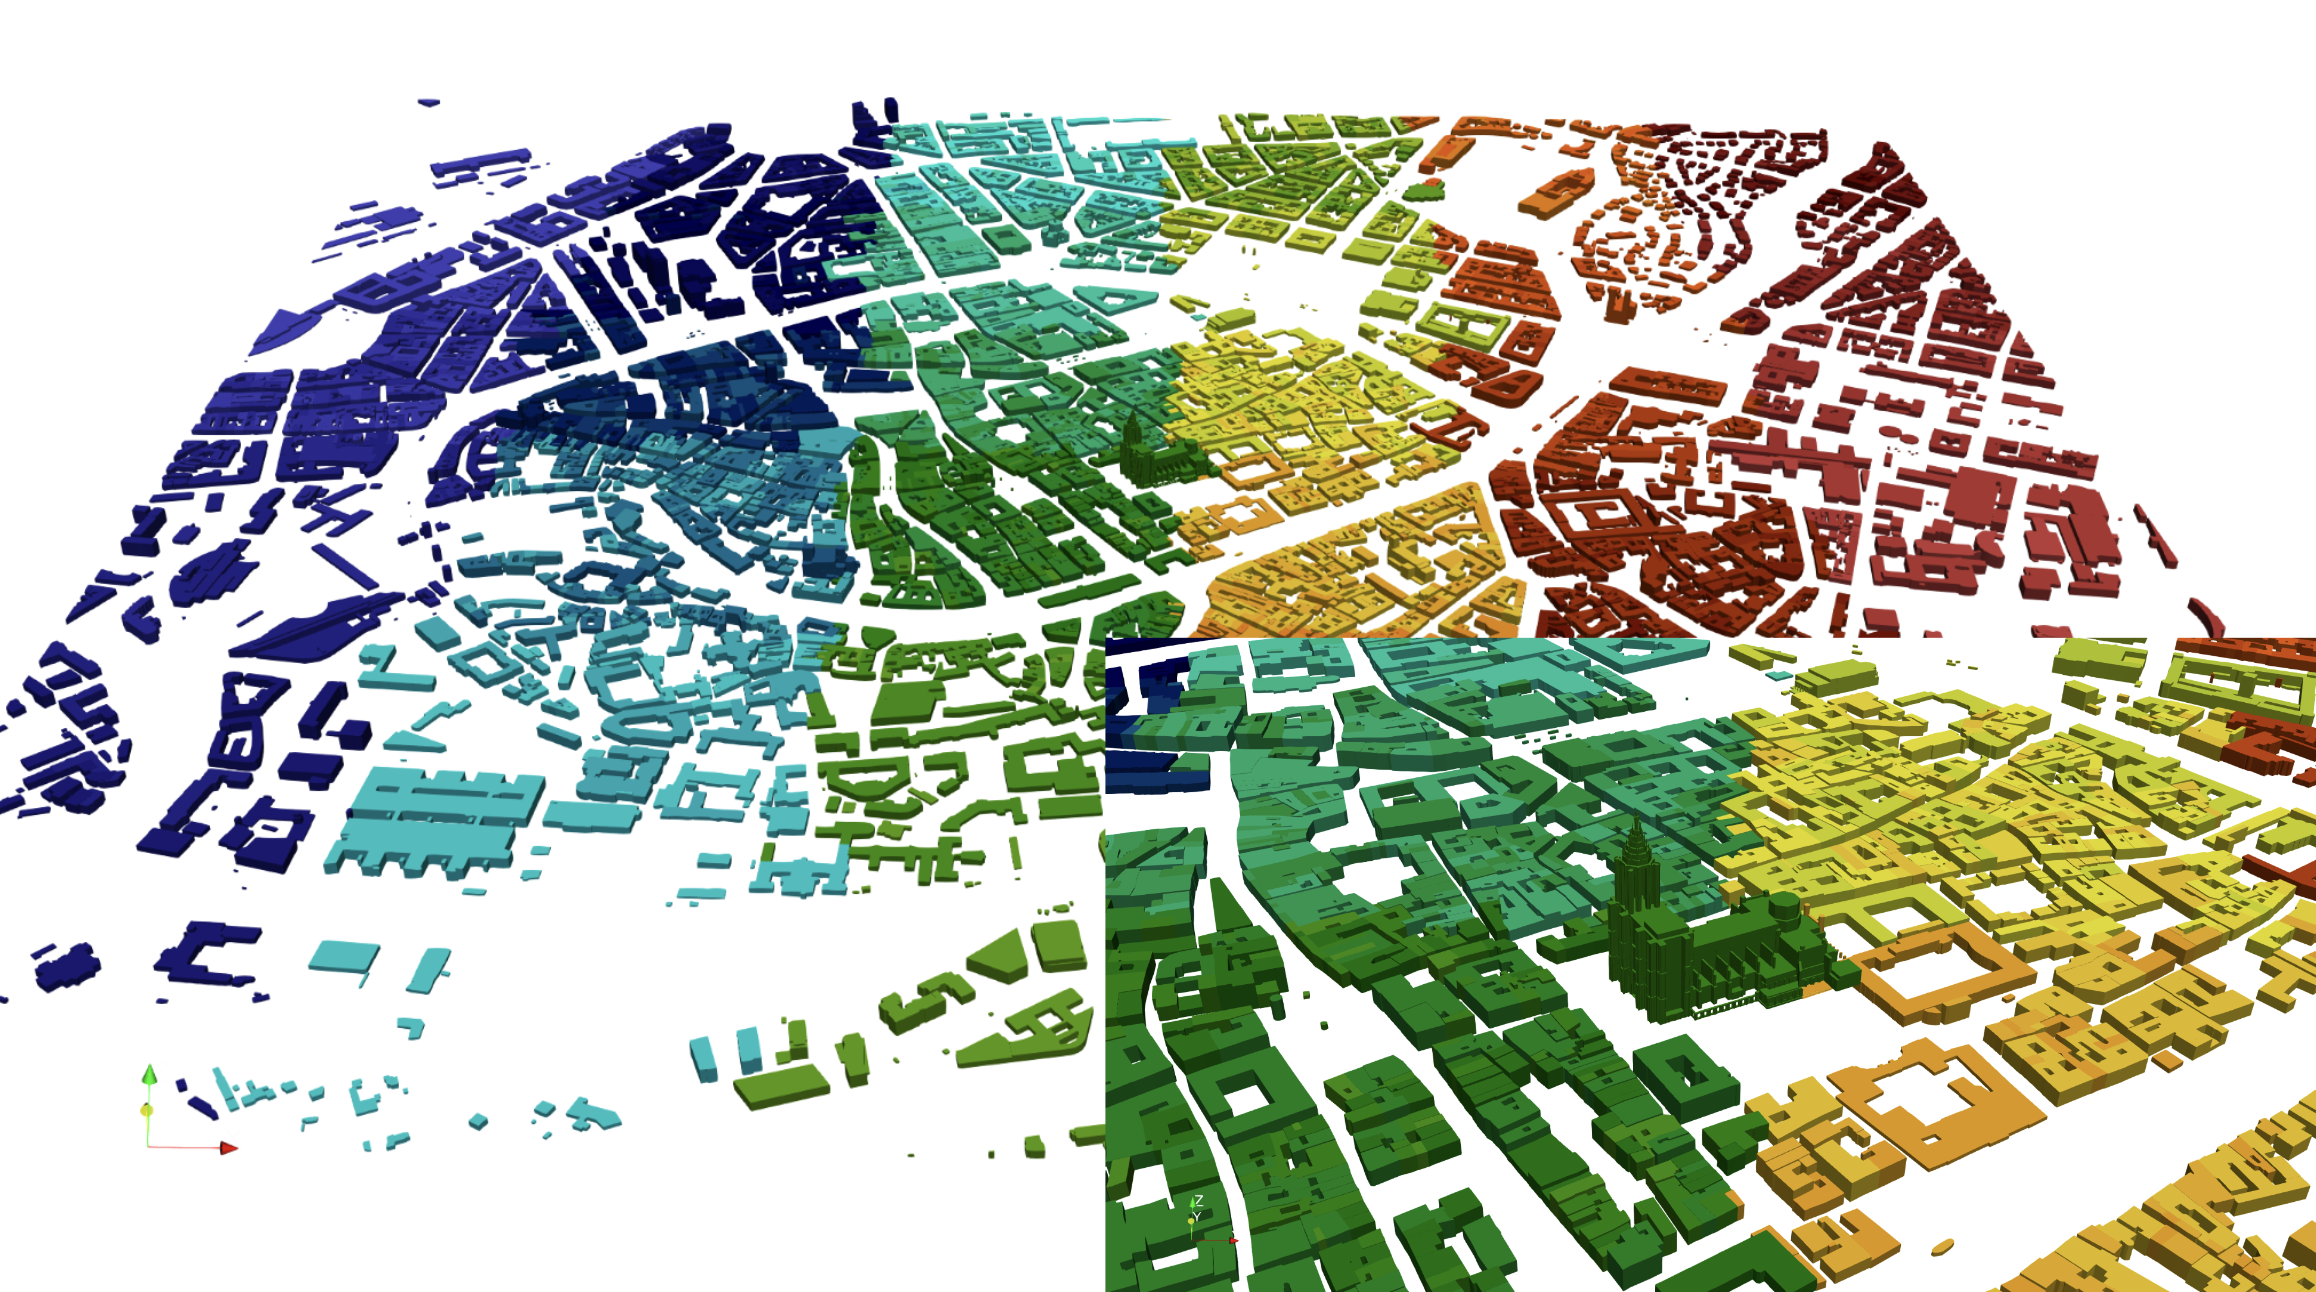
\includegraphics[width=0.46\linewidth]{CP114_img-city-strasbourg-lod0-parts.png}
}\hspace{0.02\linewidth}
%\hfill % Ensures that the images are placed side by side
\subfloat[Partitioning Case 1\label{fig:city-strasbourg-lod1-parts}]{%
  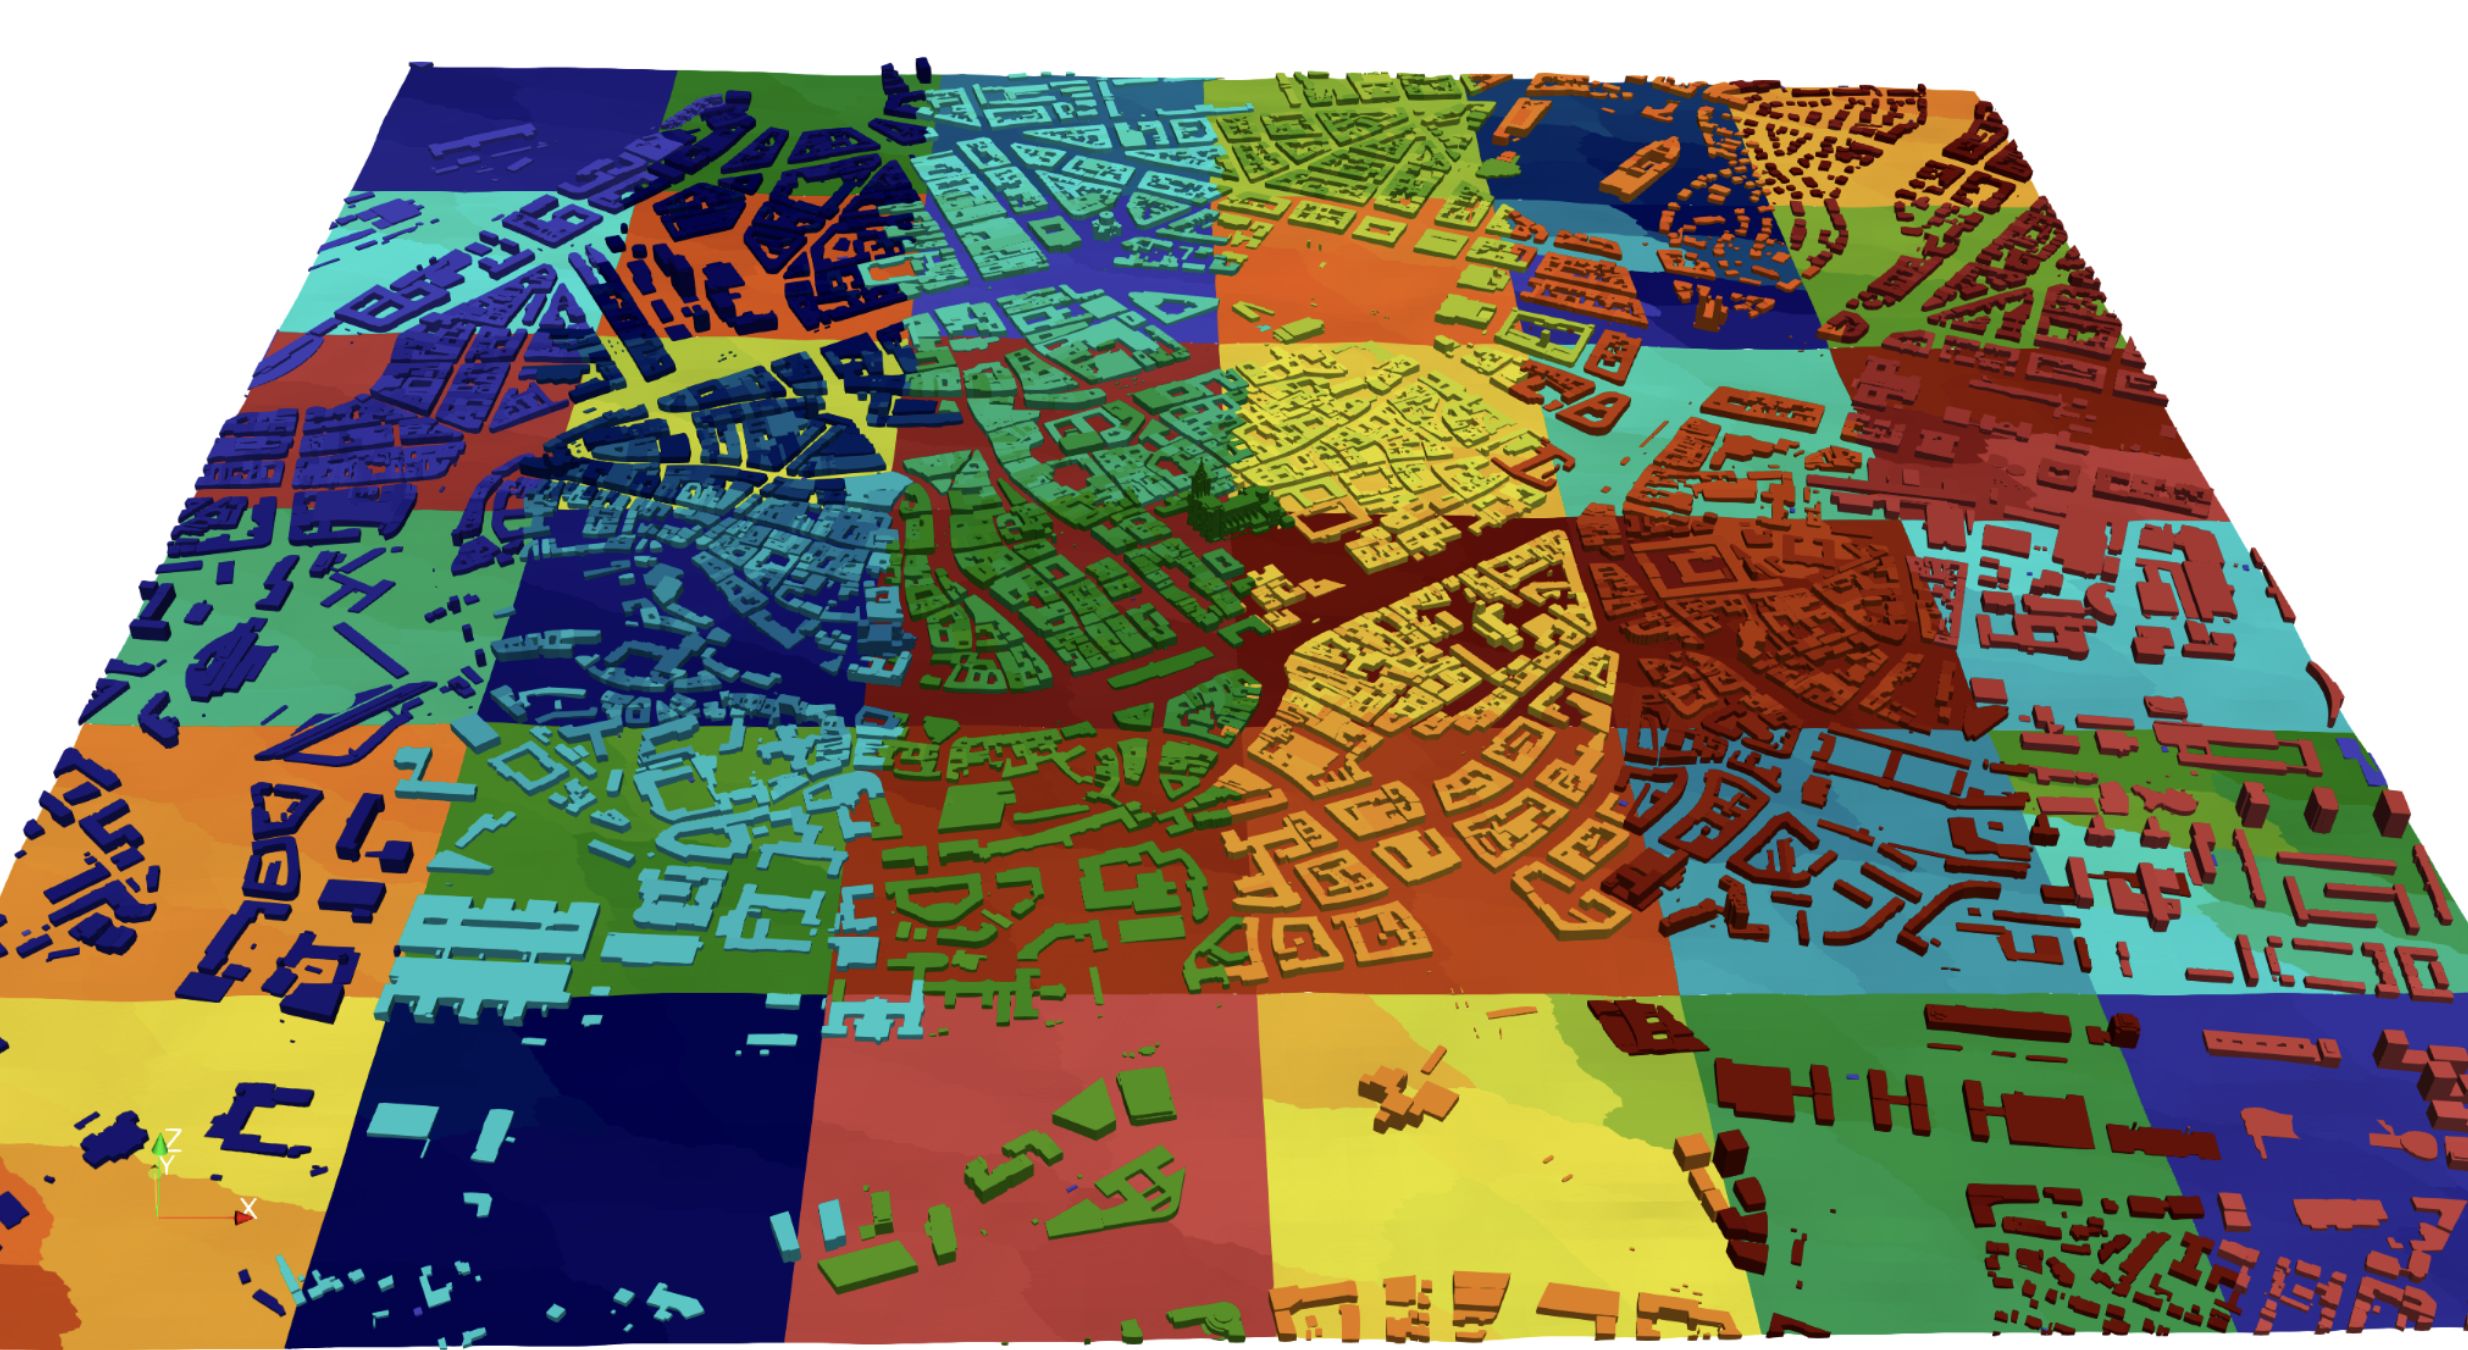
\includegraphics[width=0.46\linewidth]{CP114_img-city-strasbourg-lod1-parts.png}
}
%\subfloat[Partitioning Case 3: Large scale\label{fig:city-ny-largescale}]{%
%  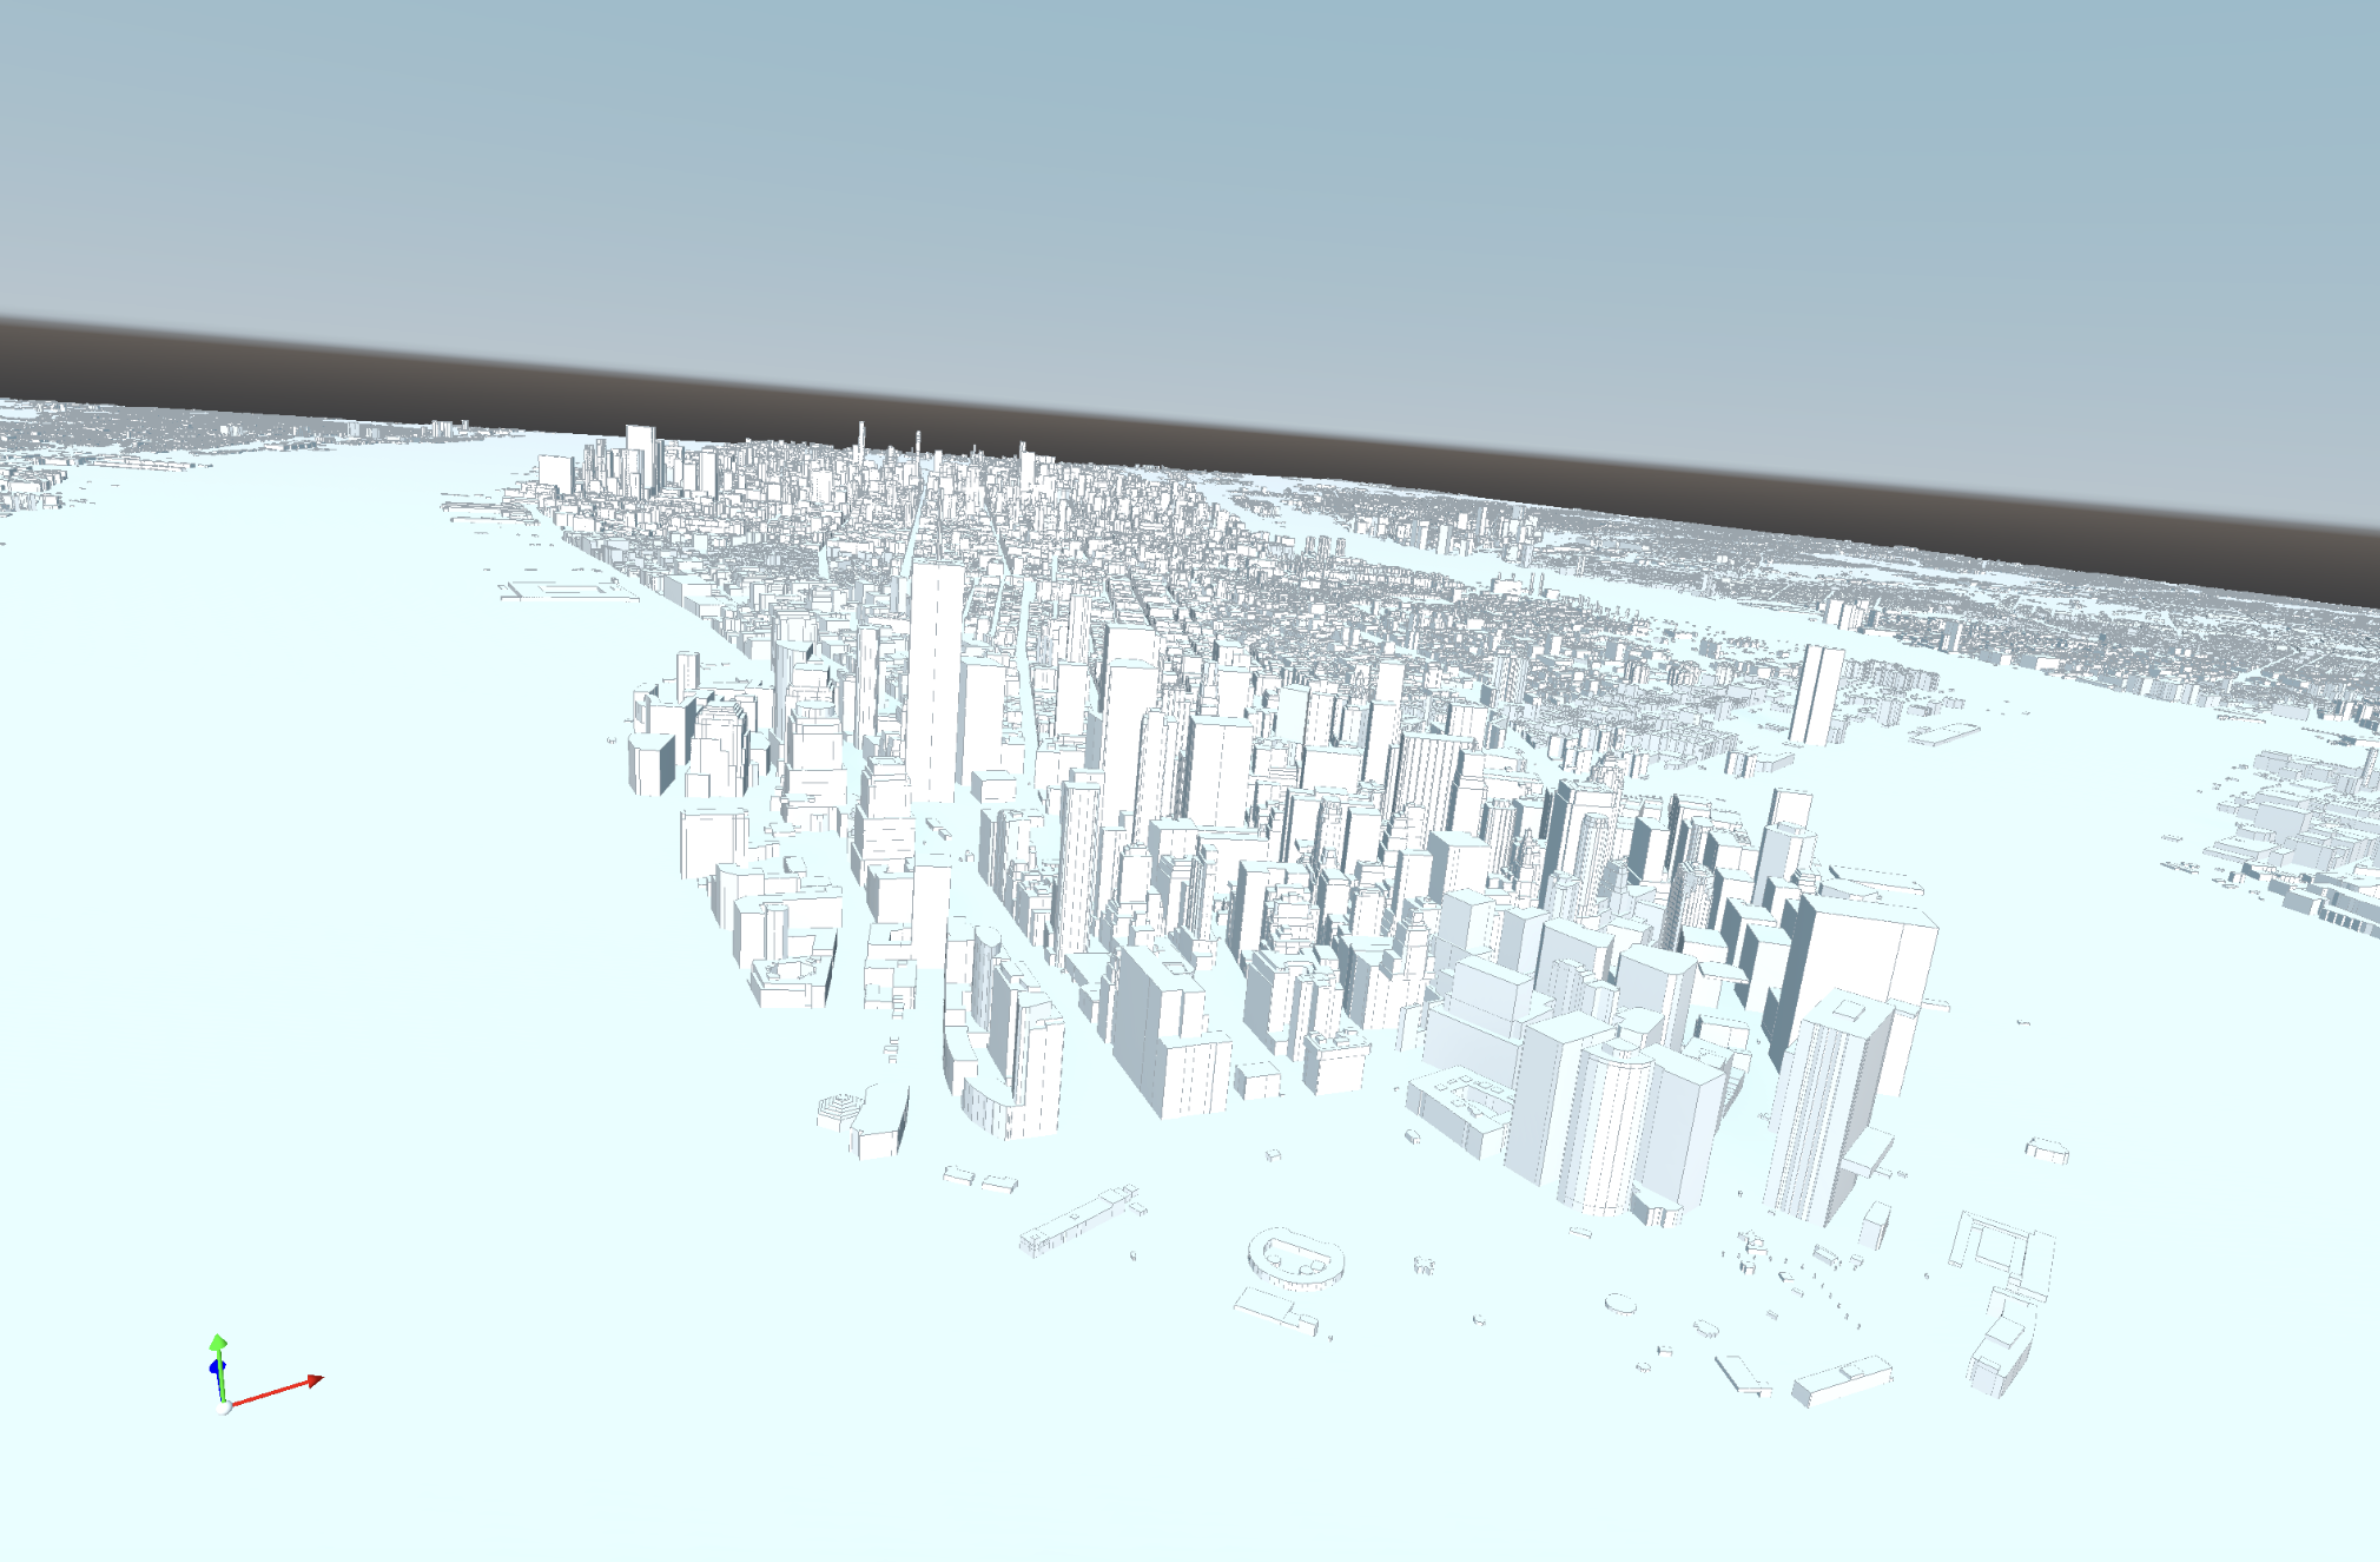
\includegraphics[width=0.4\textwidth]{CP114_img-city-newyork-largescale.png}
%}
\caption{Mesh partitioning illustrations}
\label{fig:partitioning}
\end{wrapfigure}

\Cref{fig:partitioning} illustrates the different strategies discussed previously and presents a reconstruction of New York City in \cref{fig:city-ny-largescale}. This geometric model has an area of 400 $km^2$ (20 km square side of 20 km) and has generated around 450000 buildings. This example requires the large-scale approach discussed but not yet implemented or tested.

\begin{figure}[htbp]
\centering
\subfloat[View on whole 3D mesh\label{fig:city-ny-largescale-whole}]{%
  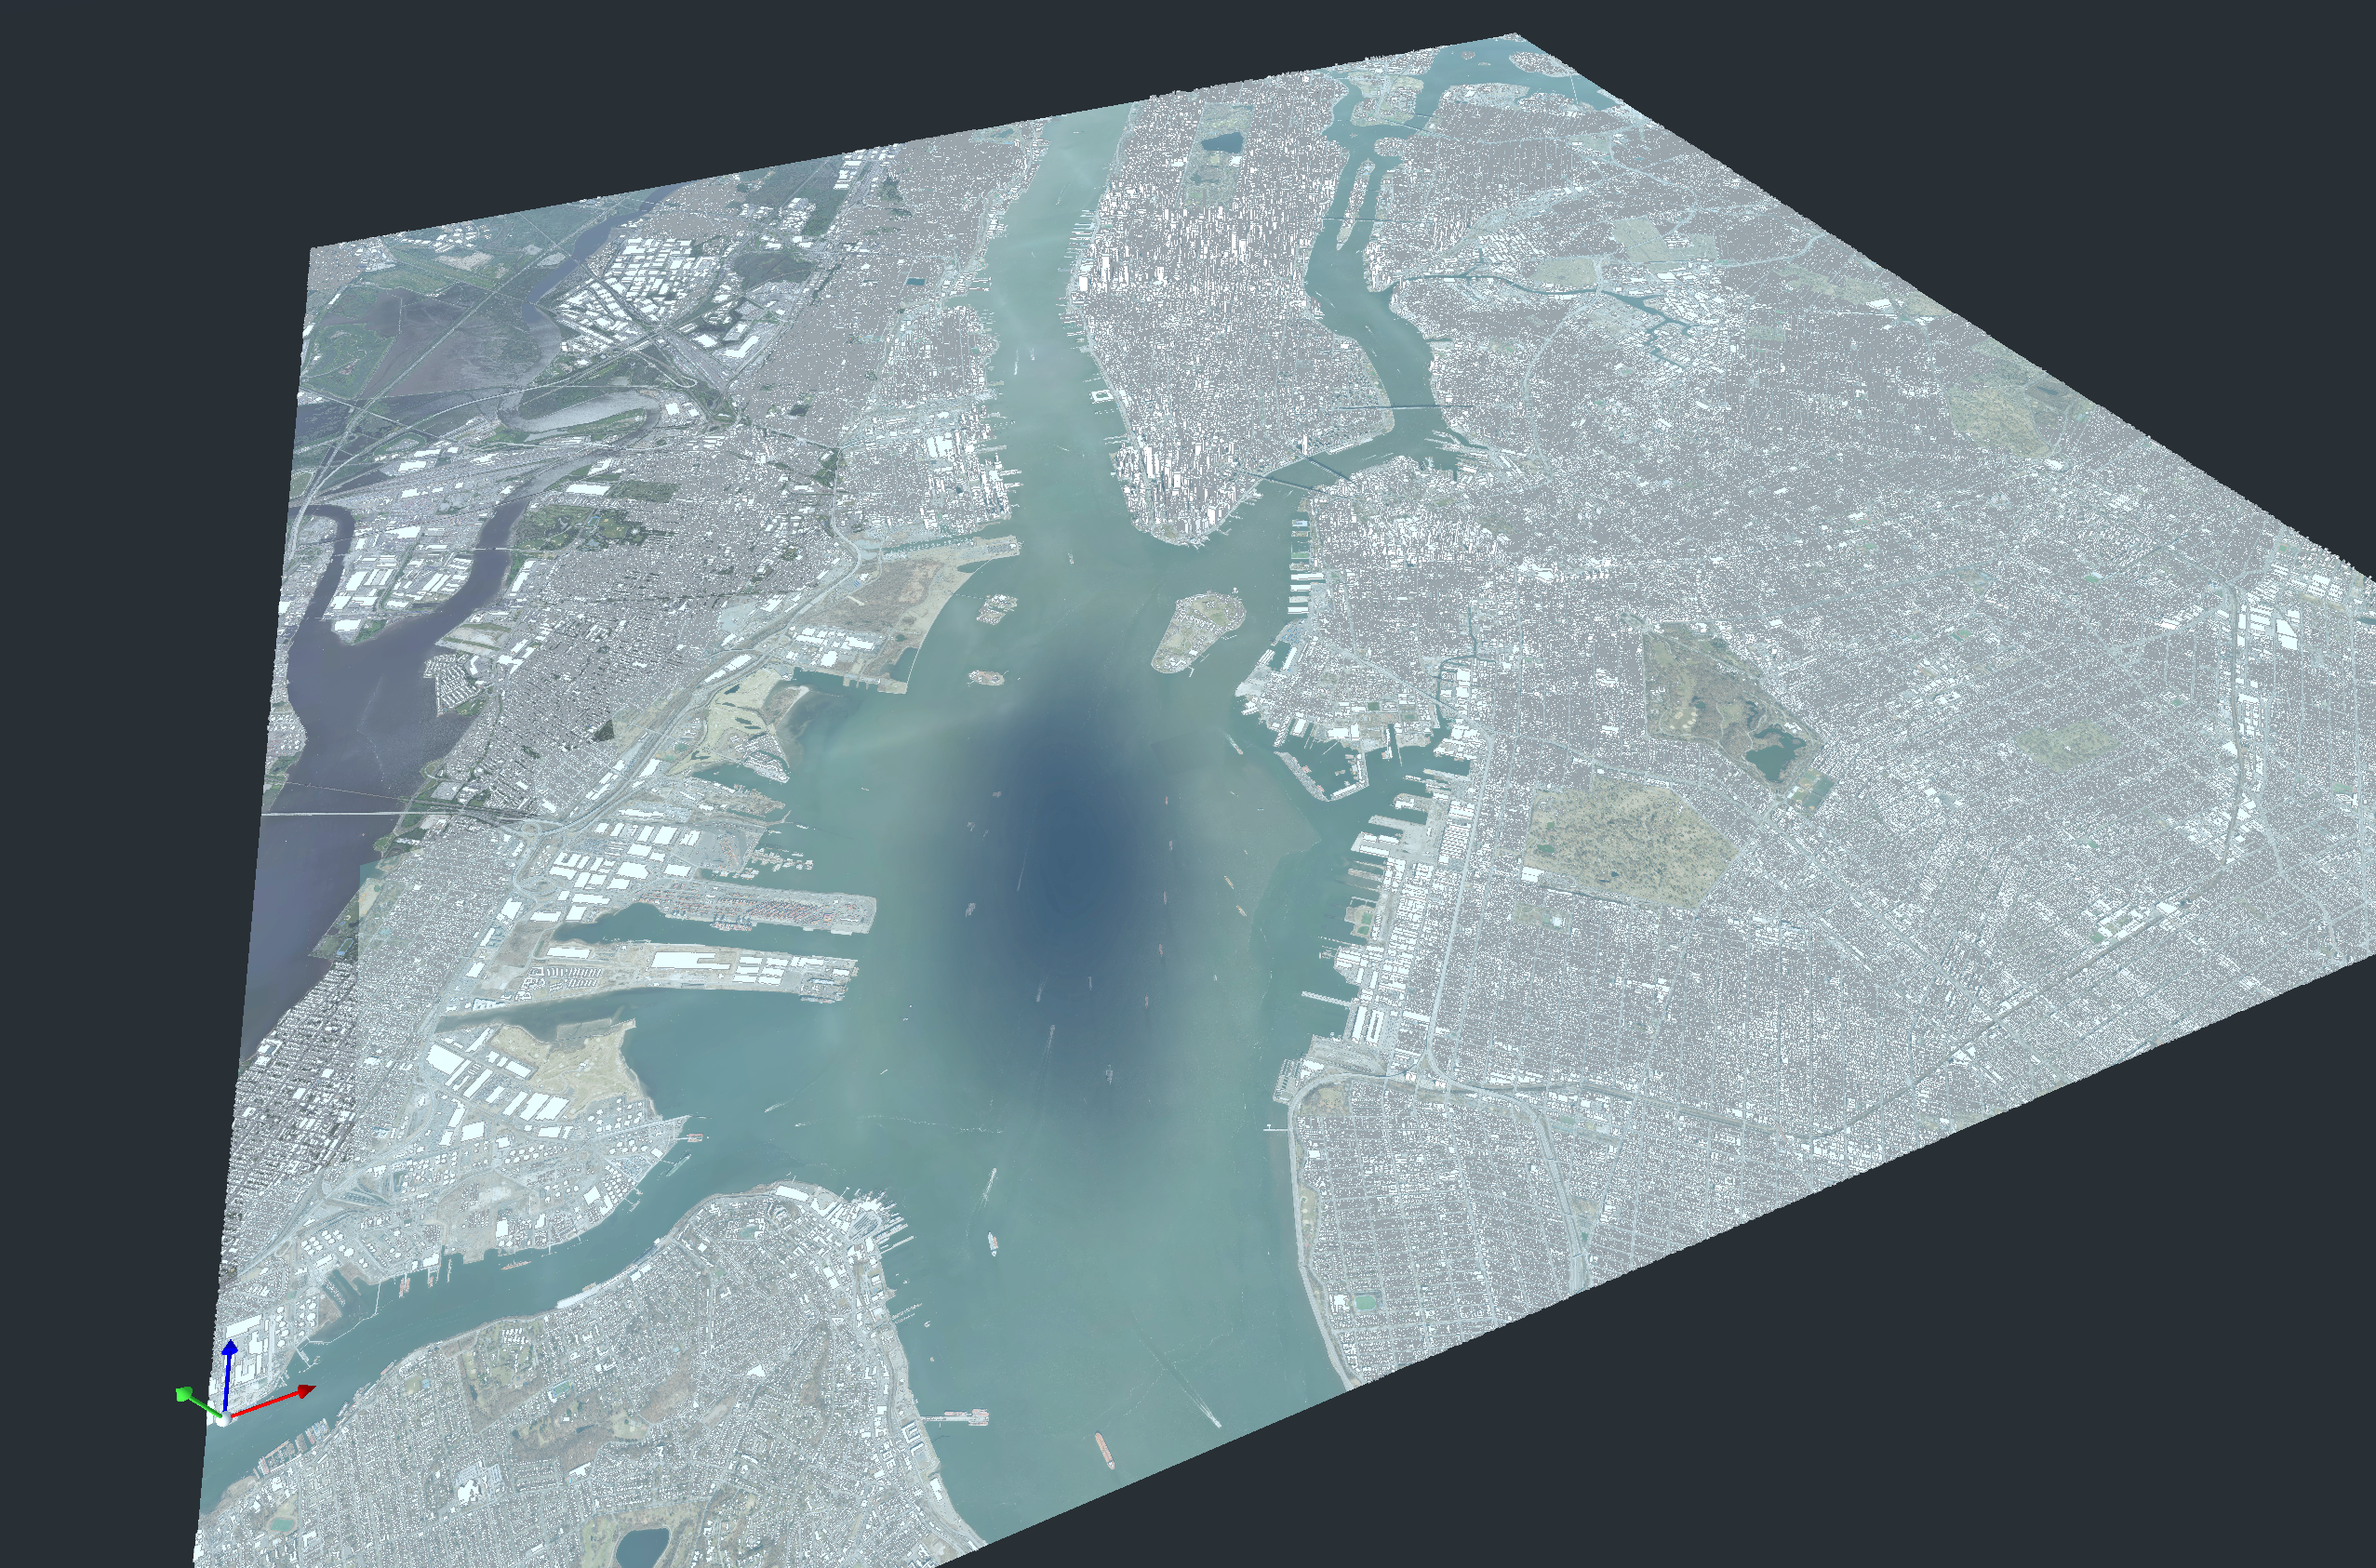
\includegraphics[width=0.45\textwidth]{CP114_img-city-newyork-largescale-whole.png}
}
\hfill
\subfloat[Zoom on Manhattan buildings\label{fig:city-ny-largescale-zoomB}]{%
  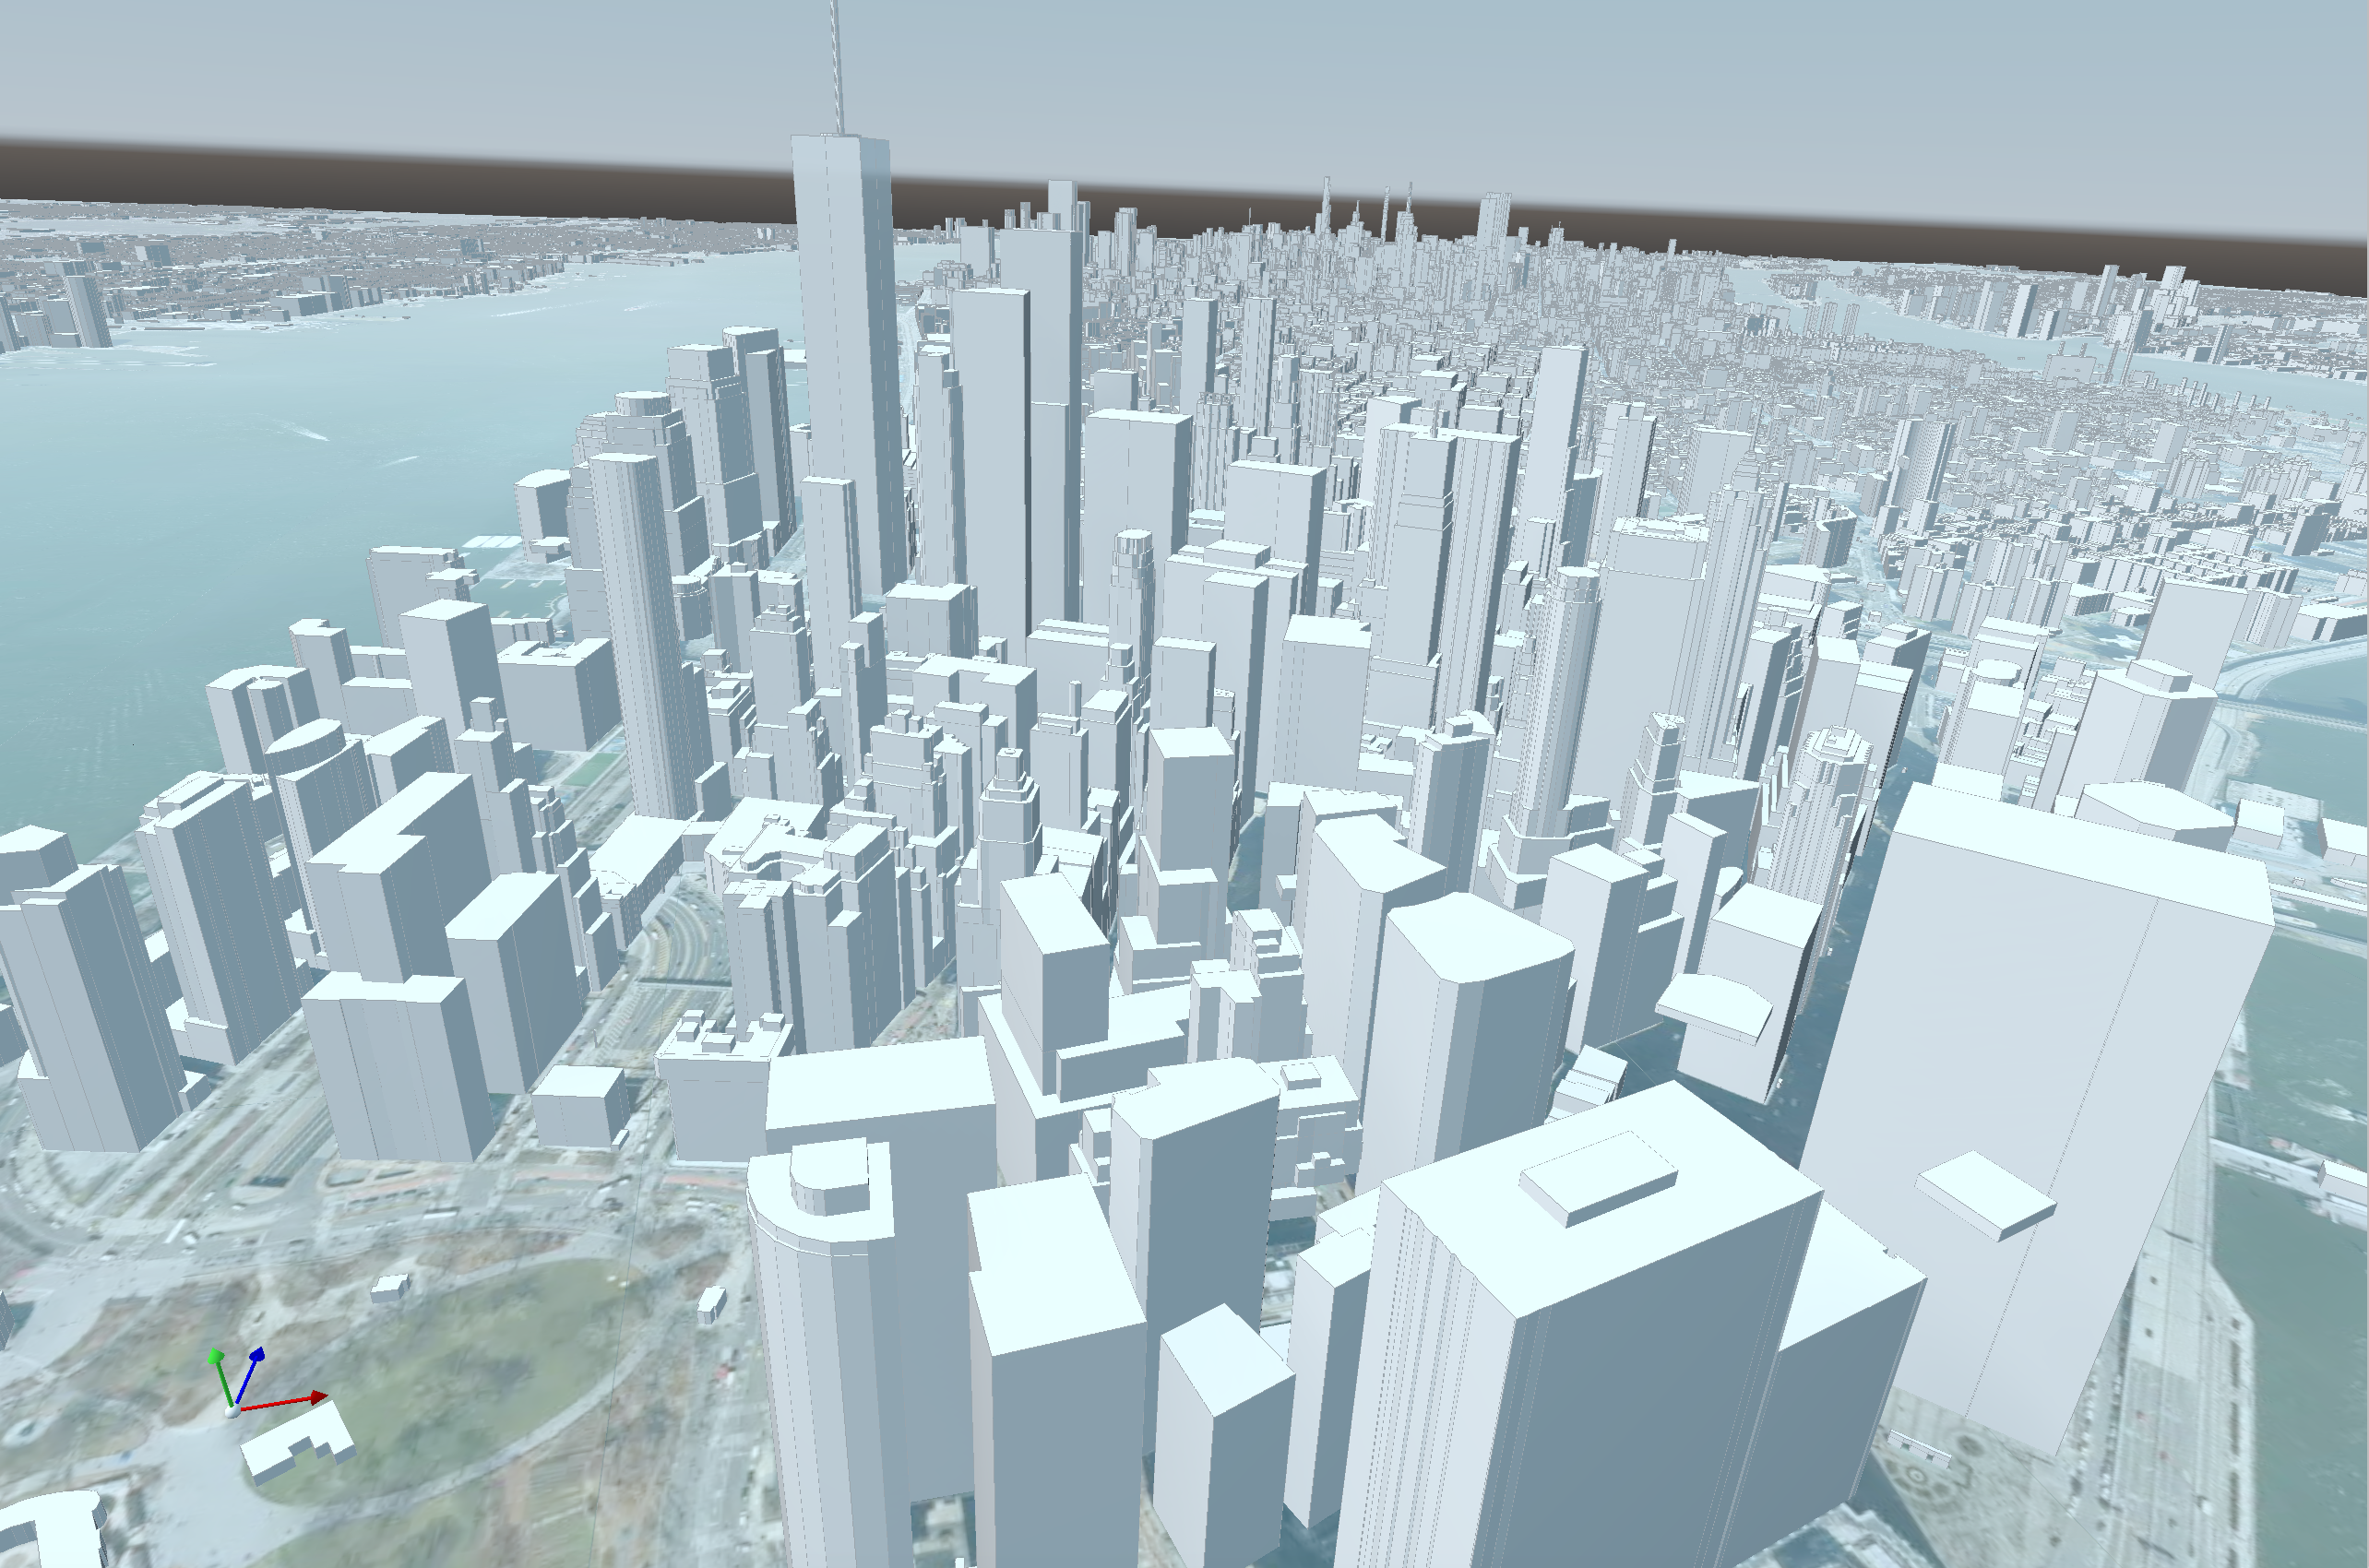
\includegraphics[width=0.45\textwidth]{CP114_img-city-newyork-largescale-zoomB.png}
}\\
\subfloat[Focus on Manhattan\label{fig:city-ny-largescale-zoomZ}]{%
  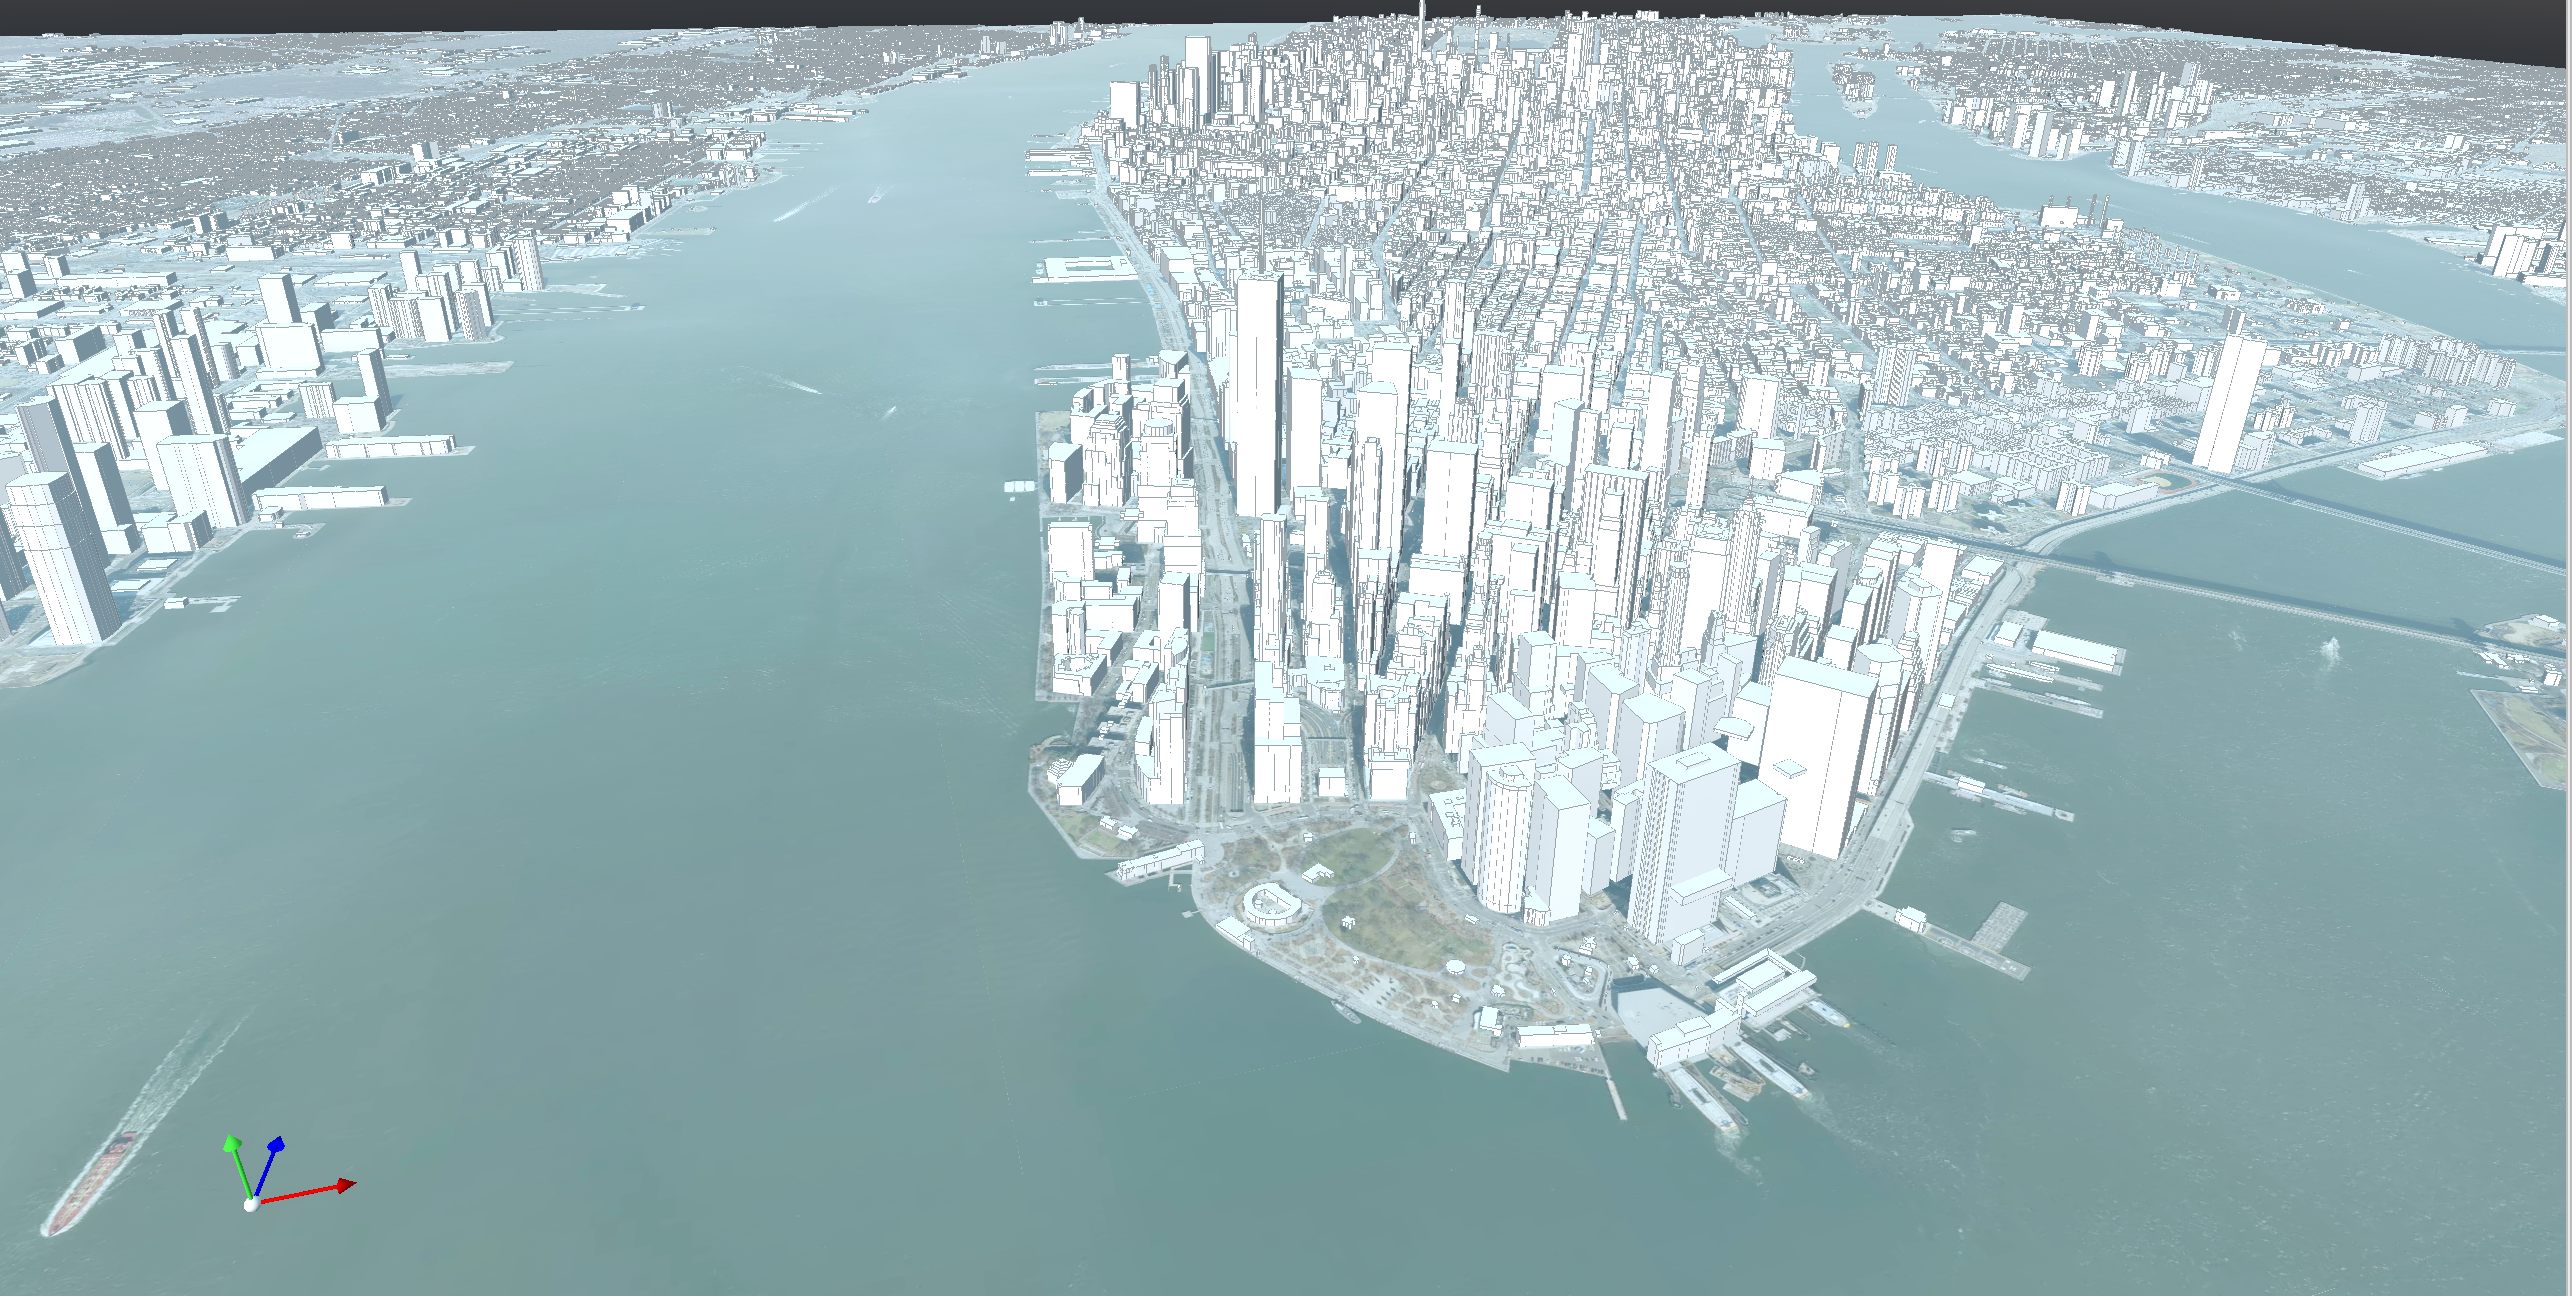
\includegraphics[width=0.45\textwidth]{CP114_img-city-newyork-largescale-zoomA.png}
}
\hfill
\subfloat[Central Park\label{fig:city-ny-largescale-zoomC}]{%
  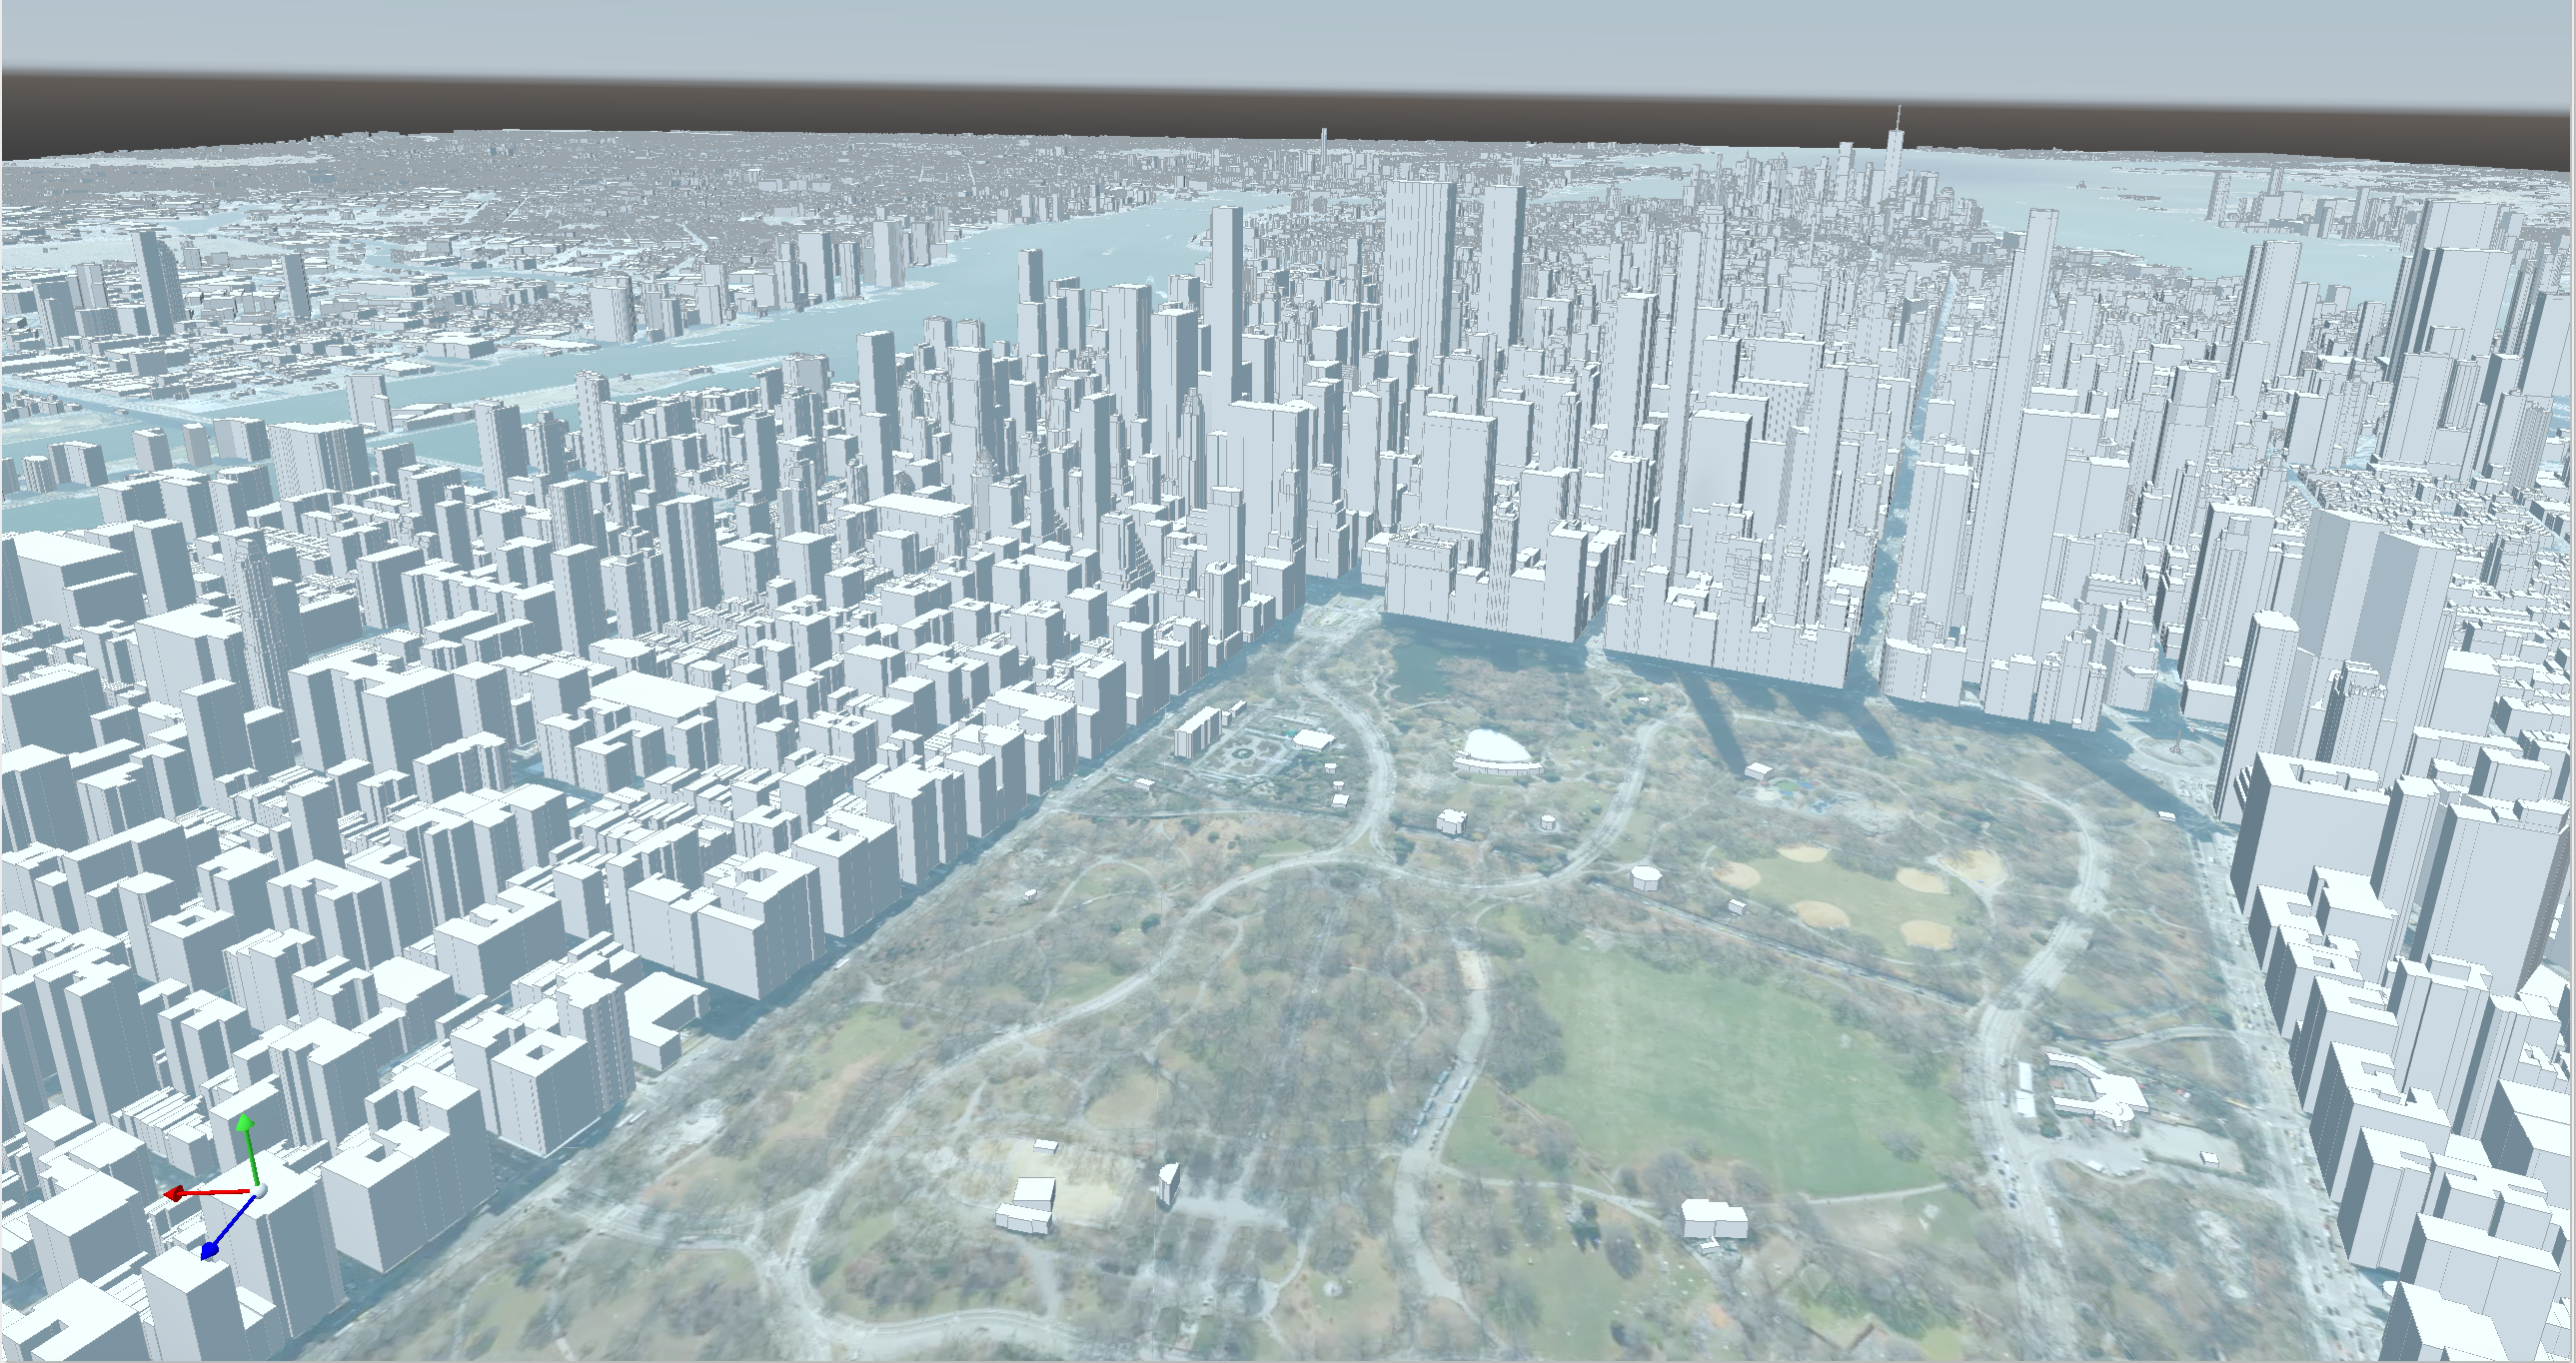
\includegraphics[width=0.45\textwidth]{CP114_img-city-newyork-largescale-zoomC.png}
}
\caption{$20 \times 20 \mathrm{km}^2\ $ geometric reconstruction of New York City (LOD-1)}
\label{fig:city-ny-largescale}
\end{figure}


\subsubsection{Conclusion on mesh construction}

Our strategy aims to improve the efficiency and scalability of the mesh generation process and enhance the fidelity and accuracy of the urban models used in simulations.

\subsection{Modeling and simulations}

We now turn to describing the physical modeling of city energy simulation.
To do this, we built on two main tools: Feel++ and Modelica.

\subsubsection{Heat transfer model in buildings}
\label{sec:heat-transfer-in-buildings}

The physical model of city buildings is currently based on a multizone model.
One zone is allocated per building floor. 
The energy balance for each zone is calculated by taking into account energy exchanges with adjacent zones and the environment.

The energy balance is written according to the first law of thermodynamics: in an isolated system, the sum of all forms of energy is constant.

\begin{equation}
    C \frac{dT}{dt} = \phi_{\mathrm{HVAC}} + \phi_{\mathrm{gain}} - \phi_{\mathrm{losses}}
\end{equation}
where
\begin{inparaenum}[\it (i)]
    \item $C \dfrac{dT}{dt}$ represents the thermal inertia of the construction, quantifying how the temperature of the zone changes over time due to its thermal mass. Specifically,
    $C$ is a measure of how much heat a material can store and release, combining the heat capacity of the construction (how much energy is required to change the temperature) with the rate of temperature change and 
    $\dfrac{dT}{dt}$ is the rate of change of temperature with respect to time. A higher thermal inertia means the construction will have a slower rate of temperature change in response to energy inputs and losses, effectively buffering temperature fluctuations;
    \item $\phi_{\mathrm{HVAC}}$ represents the energy input from the Heating, Ventilation, and Air Conditioning (HVAC) systems. It includes energy added to the zone to maintain desired temperature levels;
    \item $\phi_{\mathrm{gain}}$, referred to as free energy gain, includes solar gains (heat from sunlight) and internal gains (heat generated by occupants and equipment);
    \item $\phi_{\mathrm{losses}}$ represents the energy lost through walls, roofs, floors, and air exchanges with the environment.
\end{inparaenum}

\begin{description}
  \item[HVAC heat flow] In the version of the model at the time of writing, the HVAC system is treated as an ideal heat source, which means it adjusts its output to maintain a set temperature within the building.
  \item[Heat gain] Heat gain is the addition of energy to the building, derived from two sources: \textbf{internal heat gains} and \textbf{solar heat gains}.
  \item[Internal heat gain] The internal heat gain captures the heat produced by occupants inside the building. 
  It is modeled as a function of metabolic rate $\mathrm{Met}$ and the number of inhabitants, $d_i$, which varies over time $t$:
  \begin{equation}
    \phi_{\mathrm{int}} = \mathrm{Met} \cdot d_i(t)
  \end{equation}

\item[Solar heat gain] The total solar heat gain includes contributions from direct, diffuse, and reflected solar radiation, taking into account the building's surface characteristics and shading coefficient:
\begin{equation}
  \phi_{\mathrm{solar}} = \alpha \cdot S \cdot \left( E_{\mathrm{dir}} + E_{\mathrm{diff}} + E_{\mathrm{ref}} \right) \cdot S_C
\end{equation}
Direct solar radiation is the component of solar radiation adjusted for the angle of incidence of the sunlight:
\begin{equation}
  E_{\mathrm{dir}} = F_{\mathrm{dir}} \cdot \cos(I)
\end{equation}
Here, $F_{\mathrm{dir}}$ is the direct solar radiation, which is a function of the horizontal solar radiation measured by a weather station:
\begin{equation}
  F_{\mathrm{dir}} = \dfrac{F_{\mathrm{dir,Hz}}}{\sin(H_s)}
\end{equation}
The term $\cos(I)$ calculates the cosine of the angle of incidence of sunlight, incorporating the sun's altitude and azimuth angles as well as the building's tilt angle:
\begin{equation}
  \cos(I) = \cos(H_s) \cdot \sin(\beta) \cdot \cos(A_{zs} - A_z) + \sin(H_s) \cdot \cos(\beta)
\end{equation}
Diffuse solar radiation includes contributions from the sky dome and is adjusted for the building's tilt:
\begin{equation}
  E_{\mathrm{diff}} = F_{\mathrm{dif,Hz}} \cdot \left( \dfrac{1 + \cos(\beta)}{2} \right)
\end{equation}
Reflected solar radiation is calculated using the total horizontal radiation and the environment's albedo:
\begin{equation}
  E_{\mathrm{ref}} = \left[ F_{\mathrm{dir,Hz}} + F_{\mathrm{dif,Hz}} \right] \cdot \left( \dfrac{1 + \cos(\beta)}{2} \right) \cdot \text{albedo}
\end{equation}

\item[Conduction losses] Energy loss through walls is computed by summing the losses across all wall segments. It depends on the heat transfer coefficient, the wall area, and the temperature difference between the indoor and outdoor environments. In our current model, we simplify the calculations by not including the effects of thermal bridges, as they depend on specific information about the building's envelope, which we do not have:
\begin{equation}
  \phi_{\mathrm{wall}} = \sum_{j} U_j \cdot S_j \cdot \Delta T
\end{equation}
The convection losses are computed differently depending on the surface of the wall to which they are applied. On the interior surface, we apply a constant:
\begin{equation}
  \phi_{\mathrm{conv,int}} = \alpha_{\mathrm{conv}} \cdot \Delta T
\end{equation}
On the exterior surface, we use a forced convection model:
\begin{equation}
  \phi_{\mathrm{conv,ext}} = \left( 1.8 + 4.8 \cdot v_{\mathrm{air}} \right) \cdot \Delta T
\end{equation}

\item[Radiation losses] Radiation losses describe the heat energy lost due to thermal radiation, impacting both energy efficiency and thermal comfort.
We differentiate between the exterior of the wall that exchanges with the sky and the interior where the walls exchange with each other.
namely, for the exterior radiation exchange:
\begin{equation}
  \phi_{\mathrm{net,sky}} = \varepsilon_i \cdot \sigma \cdot \left( T_i^4 - T_{\mathrm{sky}}^4 \right)
\end{equation}
and for the interior radiation exchange:
\begin{equation}
  J[i] = \varepsilon_i \cdot \sigma \cdot T_i^4 + \left( 1.0 - \varepsilon_i \right) \cdot \sum_{j=1}^{n} F[i,j] \cdot J[j]
\end{equation}
where the radiative heat exchange $J[i]$ includes two terms:
\begin{inparaenum}[\it (i)]
    \item $\varepsilon_i \cdot \sigma \cdot T_i^4$, which calculates the heat radiated by surface $i$ where $\varepsilon_i$ measures how effectively the surface emits radiation and $T_i^4$ reflects that radiative heat loss increases rapidly with temperature; and
    \item $\left( 1.0 - \varepsilon_i \right) \cdot \sum_{j=1}^{n} F[i,j] \cdot J[j]$, which accounts for the heat absorbed from other surfaces $j$ within the zone. The factor $\left( 1.0 - \varepsilon_i \right)$ adjusts for the fraction of incoming radiation not emitted by surface $i$.
\end{inparaenum}
The net radiation flow is given by:
\begin{equation}
  \phi_{\mathrm{net,int}}[i] = S \cdot \dfrac{\varepsilon_i}{1.0 - \varepsilon_i} \cdot \left( \sigma \cdot T_i^4 - J[i] \right)
\end{equation}
Net radiation flow $Q_{\mathrm{flow}}[i]$ considers:
\begin{inparaenum}[\it (i)]
    \item $\dfrac{\varepsilon_i}{1.0 - \varepsilon_i} \cdot \left( \sigma \cdot T_i^4 - J[i] \right)$, which calculates the net heat flow due to radiation for surface $i$, considering the difference between the heat emitted by the surface and the heat received from other surfaces. The ratio $\dfrac{\varepsilon_i}{1.0 - \varepsilon_i}$ scales the net flow based on the emissivity of the surface.
\end{inparaenum}

\item[Air change] This term represents the energy loss due to air exchange between the zone and the exterior:
\begin{equation}
  \phi_{\mathrm{air}} = 0.34 \cdot Q_v \cdot \Delta T
\end{equation}
\end{description}
The described thermal models are implemented using the Modelica language, which is an object-oriented, equation-based language well-suited for modeling complex physical systems. 
These models are then transformed into Functional Mock-up Units (FMUs) compliant with the Functional Mock-up Interface (FMI) standard. 
FMUs encapsulate the models and enable them to be shared and integrated across different simulation environments.


\paragraph{Conclusion} By integrating these models within a high-performance computing framework, it is possible to simulate the thermal behavior of city-scale building clusters.
This facilitates the assessment of energy consumption, thermal comfort, and the impact of various energy-saving strategies under different environmental conditions and operational scenarios.

\subsubsection{KUB is based on the Feel++ toolchain}

Feel++ is a comprehensive framework designed to tackle problems based on Ordinary Differential Equations (ODEs) and Partial Differential Equations (PDEs). 
Using modern C++ (C++17 and C++20) standards coupled with a Python layer through Pybind11, Feel++ enables seamless parallelism and is equipped with default communicators that simplify handling complex computational tasks.
The framework's versatility is evident in its deployment across various platforms, including research and educational environments and cloud services tailored for high-performance computing needs.

Key features of the Feel++ framework encompass an extensive range of numerical methods designed to address Partial Differential Equations (PDEs), see~\cite{christophe_prudhomme_feelppfeelpp_2024}. 
These methods include continuous Galerkin (cG), discontinuous Galerkin (dG), hybrid discontinuous Galerkin (hdG), and reduced basis methods (rb/mor). 
A Domain Specific Language (DSL) for Galerkin methods significantly enhances the ease of implementing and experimenting with new numerical methods. 
The de Rham complex provides a comprehensive toolkit for constructing finite element spaces of arbitrary order, facilitating precise mathematical modeling. 
The framework's automatic differentiation and symbolic integration capabilities effectively bridge the gap between mathematical expressions and their computational implementation.
Feel++ supports diverse applications, from fluid dynamics and structural mechanics to heat transfer and electrostatics, demonstrating its flexibility and broad applicability.
Furthermore, its integration with Specx for task-based parallel execution optimizes performance and scalability on modern computational architectures.

%\paragraph{Simulation Tools and Applications}
%Feel++ comes equipped with various toolboxes tailored for specific application domains, offering pre-built scenarios for fluid dynamics, solid mechanics, and electromagnetism, among others. These toolboxes are designed to provide robust and efficient solutions, leveraging the capabilities of Feel++ to address complex multi-physics problems in real-world scenarios.

Documentation and further details can be accessed through Feel++ Toolboxes Documentation\footnote{\url{https://docs.feelpp.org/toolboxes/latest/}}.
This powerful toolchain is essential for KUB.

\subsubsection{Computing Shading Masks and View Factors with Feel++}

In city energy simulations, the computation of shading masks and view factors is crucial for accurately modeling the impact of solar radiation on building surfaces. Shading masks quantify the percentage of blocked solar radiation for each building surface (including walls and roofs) depending on the sun's direction. This is influenced by nearby structures such as other buildings, vegetation, and urban furniture. The view factors describe the fraction of radiation that leaves one surface and strikes another, essential for calculating radiative heat exchanges between building surfaces.

\paragraph{Numerical Methods and Challenges}
Both shading masks and view factors are computed using Monte Carlo and ray tracing techniques, which allow for handling complex geometries with various obstructions. Despite being purely geometric quantities, these calculations face significant challenges such as:
\begin{inparaenum}[\it (i)]
    \item Efficient computation of integrals for view factors, especially when considering specular surfaces that require multiple ray bounces.
    \item Managing large-scale mesh computations and data storage, particularly when detailed urban environments are modeled.
\end{inparaenum}


\paragraph{Implementation in Feel++}
Feel++ employs Monte Carlo methods for solar mask computations across multiple CPU cores, incorporating dynamic shading into building energy simulations. \Cref{fig:solar-masks-vf} shows:
\textit{(i)} an east-facing mask (\cref{fig:sm-building-east});
\textit{(ii)} a whole-building mask (\cref{fig:sm-whole-building});
\textit{(iii)} a city-scale mask for Strasbourg (\cref{fig:sm-strasbourg}); and
\textit{(iv)} a 2D benchmark~\cite{van_eck_surface_2016} used for view factors (\cref{fig:view-factor}).

Each mask's grayscale ranges from 0 (white, no obstruction) to 1 (black, total obstruction). Intermediate shades denote partial shading from adjacent buildings or features. 
The chosen LOD (level of discretization) determines mask resolution, as illustrated in \cref{fig:sm-building-east,fig:sm-whole-building}.%In \cref{fig:sm-building-east} (LOD-0), we see a coarser discretization with larger, generalized angular segments, leading to more abrupt transitions between obstructed and non-obstructed areas. In contrast, \cref{fig:sm-whole-building} (LOD-1) provides a finer level of detail, capturing more granular variations in solar accessibility across different sun angles. These masks help quantify the solar exposure of building surfaces over time, which is critical for accurately modeling heat gains and understanding the thermal dynamics of urban environments.

\begin{figure}[ht]
\centering
\subfloat[LOD-0\label{fig:sm-building-east}]{%
  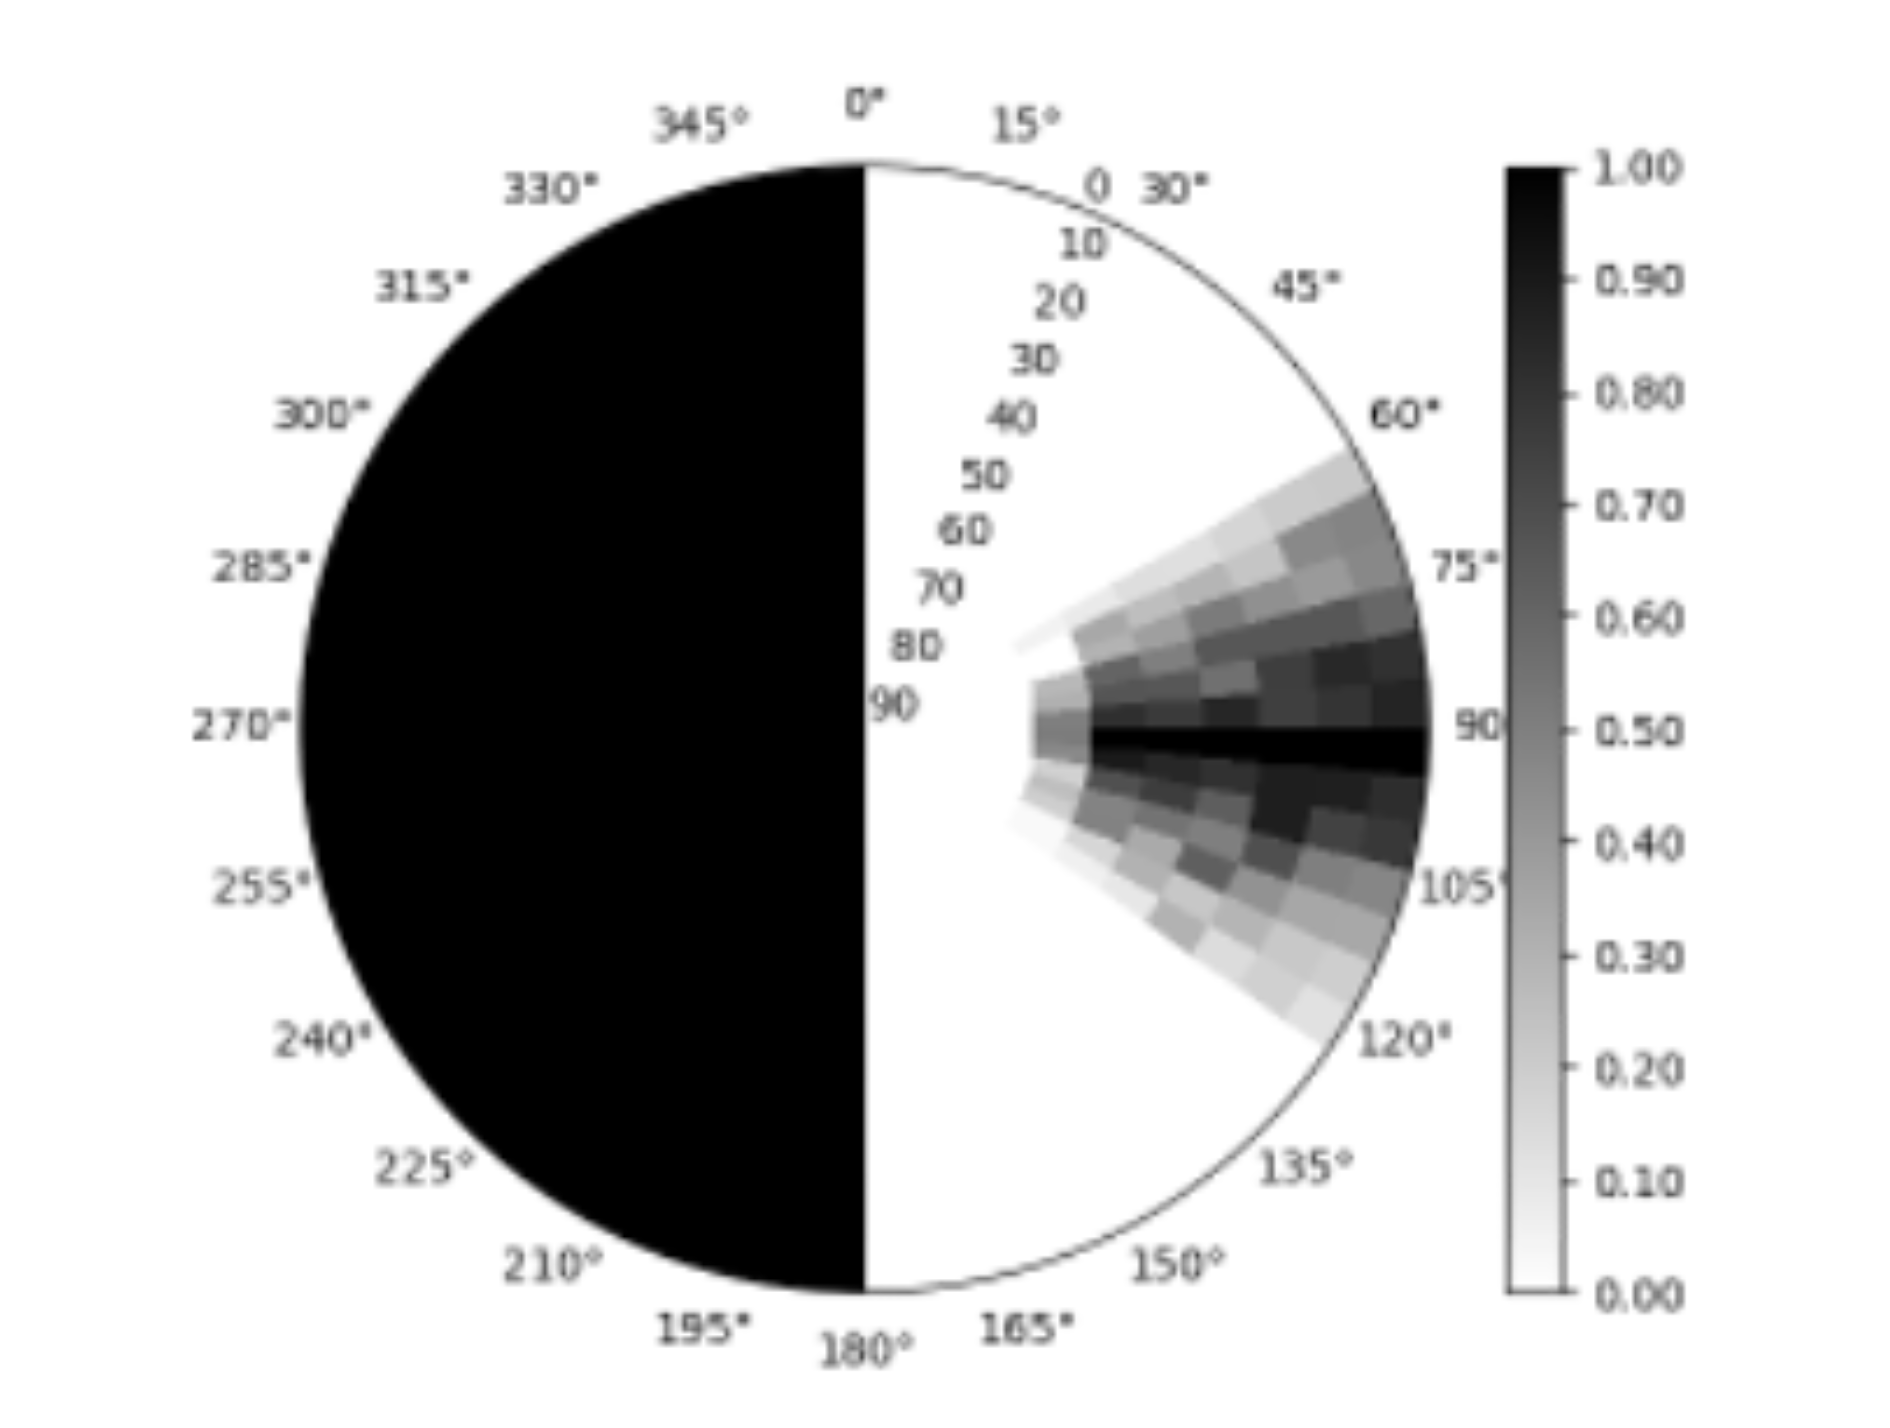
\includegraphics[width=0.45\textwidth]{CP114_img-solar-masks-east-facing.png}
}
\hfill
\subfloat[LOD-1\label{fig:sm-whole-building}]{%
  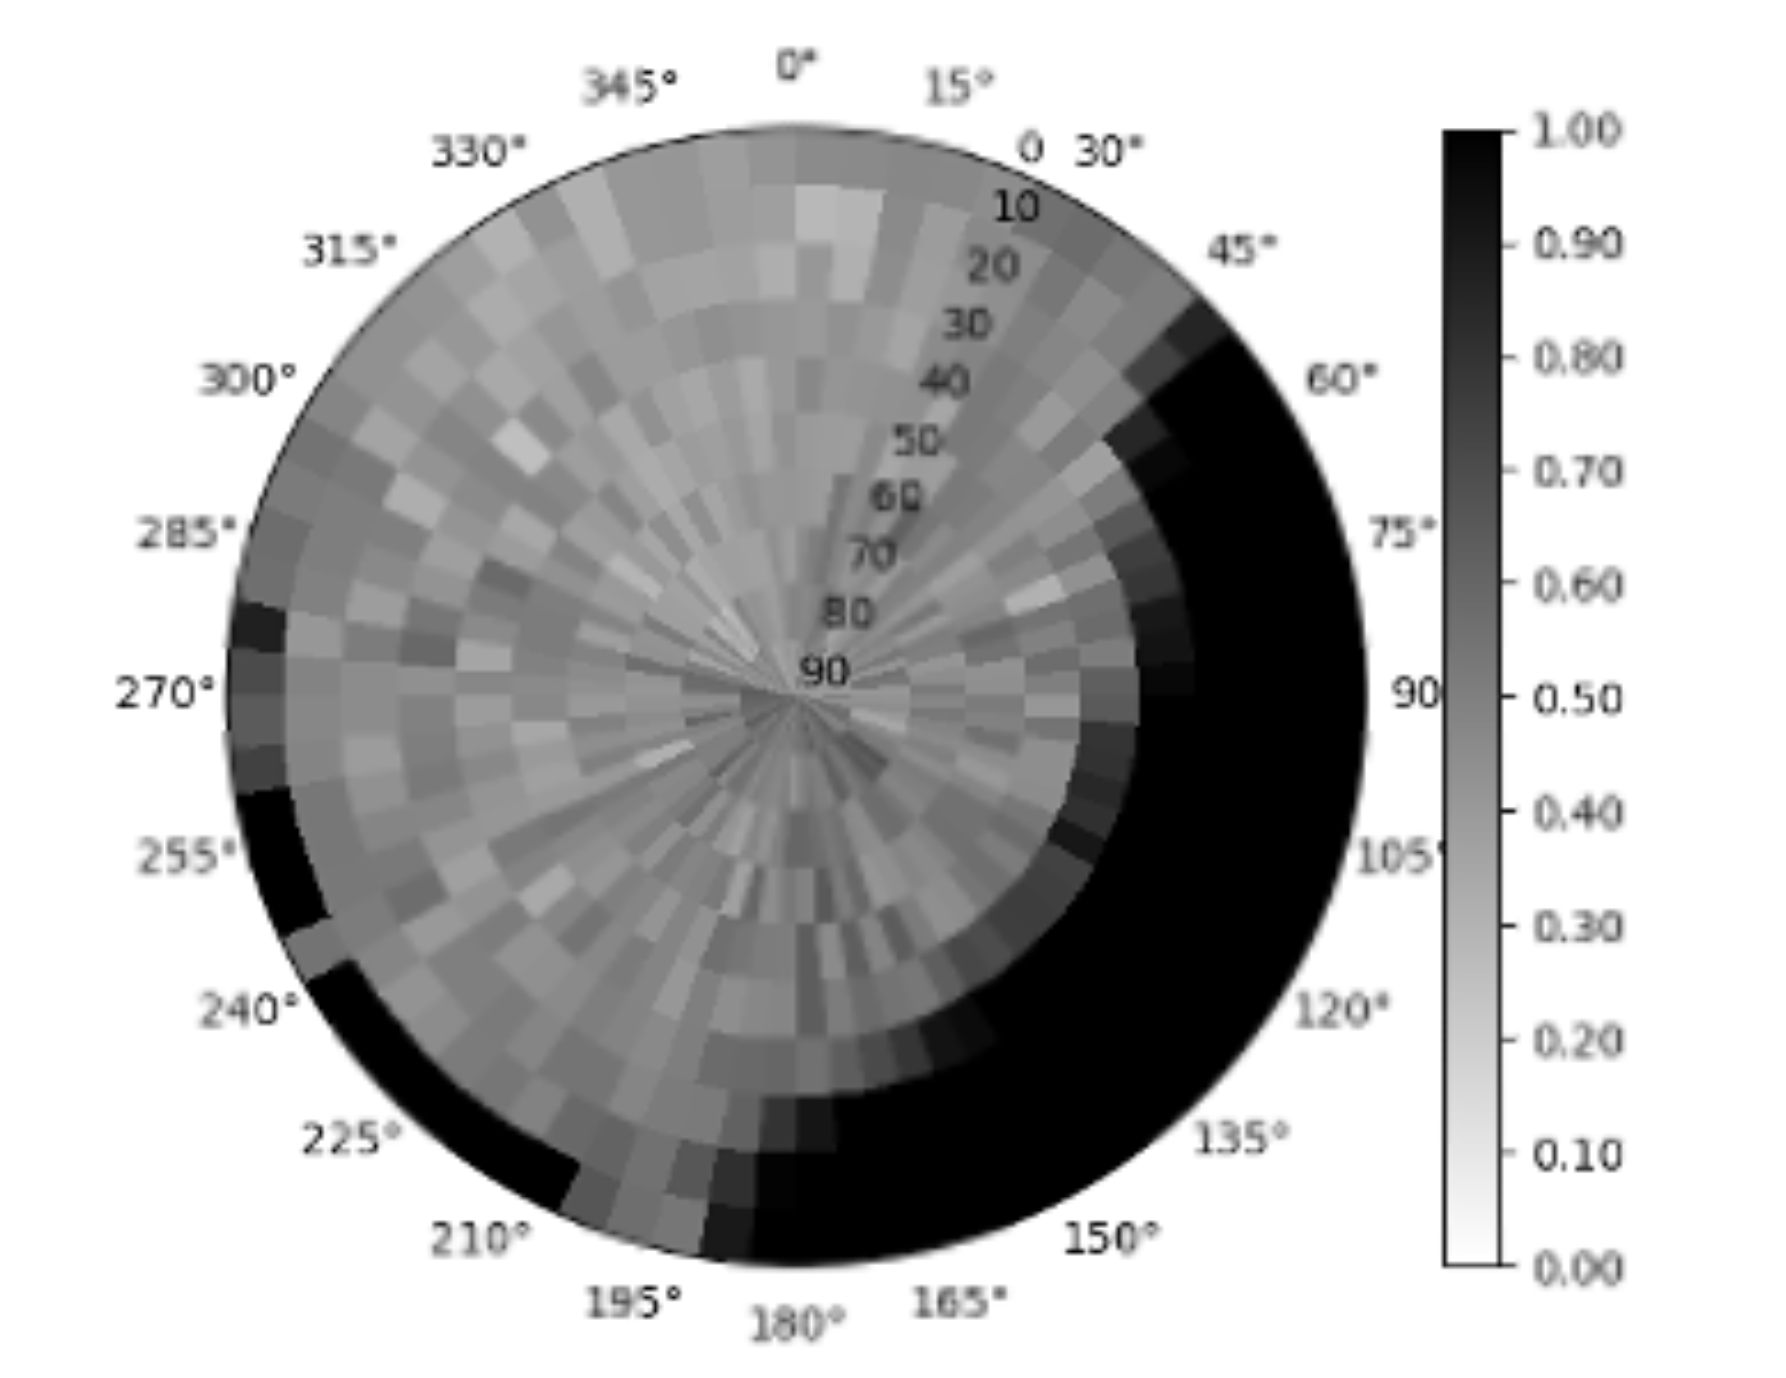
\includegraphics[width=0.45\textwidth]{CP114_img-solar-masks-whole-building.png}
}\\
\subfloat[LOD-1 Large scale\label{fig:sm-strasbourg}]{%
  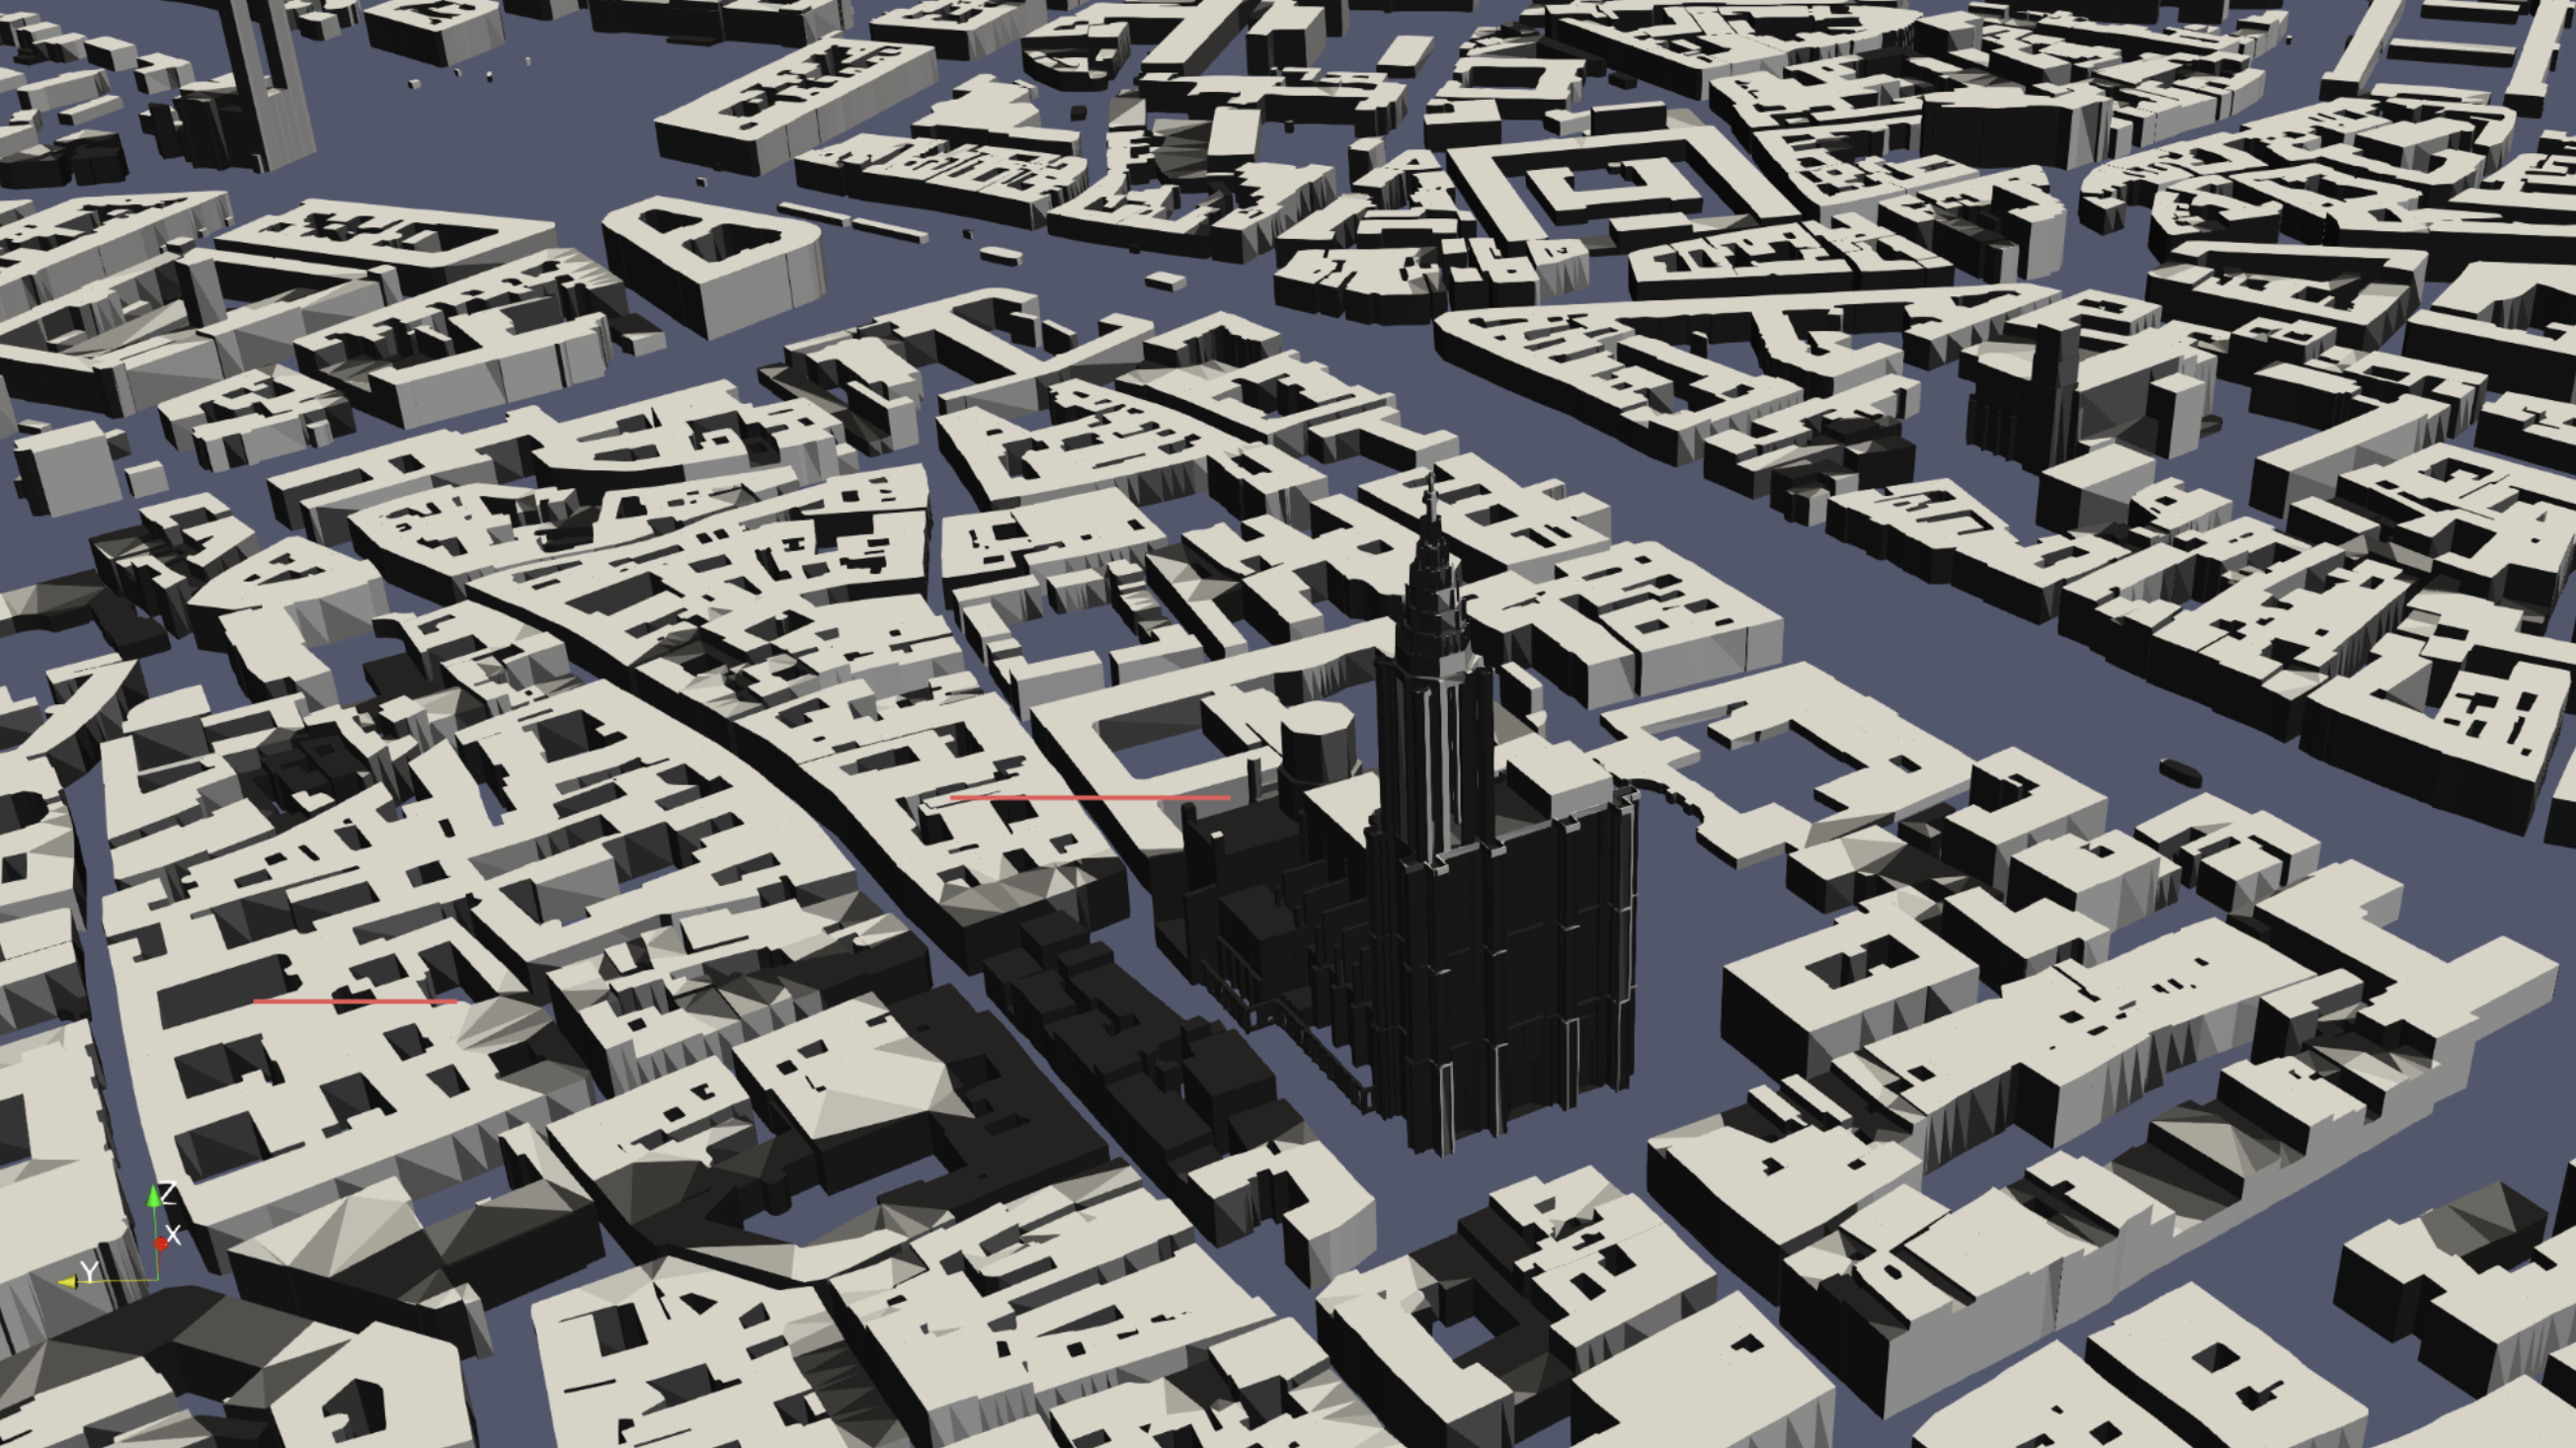
\includegraphics[width=0.45\textwidth]{CP114_img-solar-masks-strasbourg.png}
}
\hfill
\subfloat[Heat transfer benchmark in 2D including view factors~\cite{van_eck_surface_2016}\label{fig:view-factor}]{%
  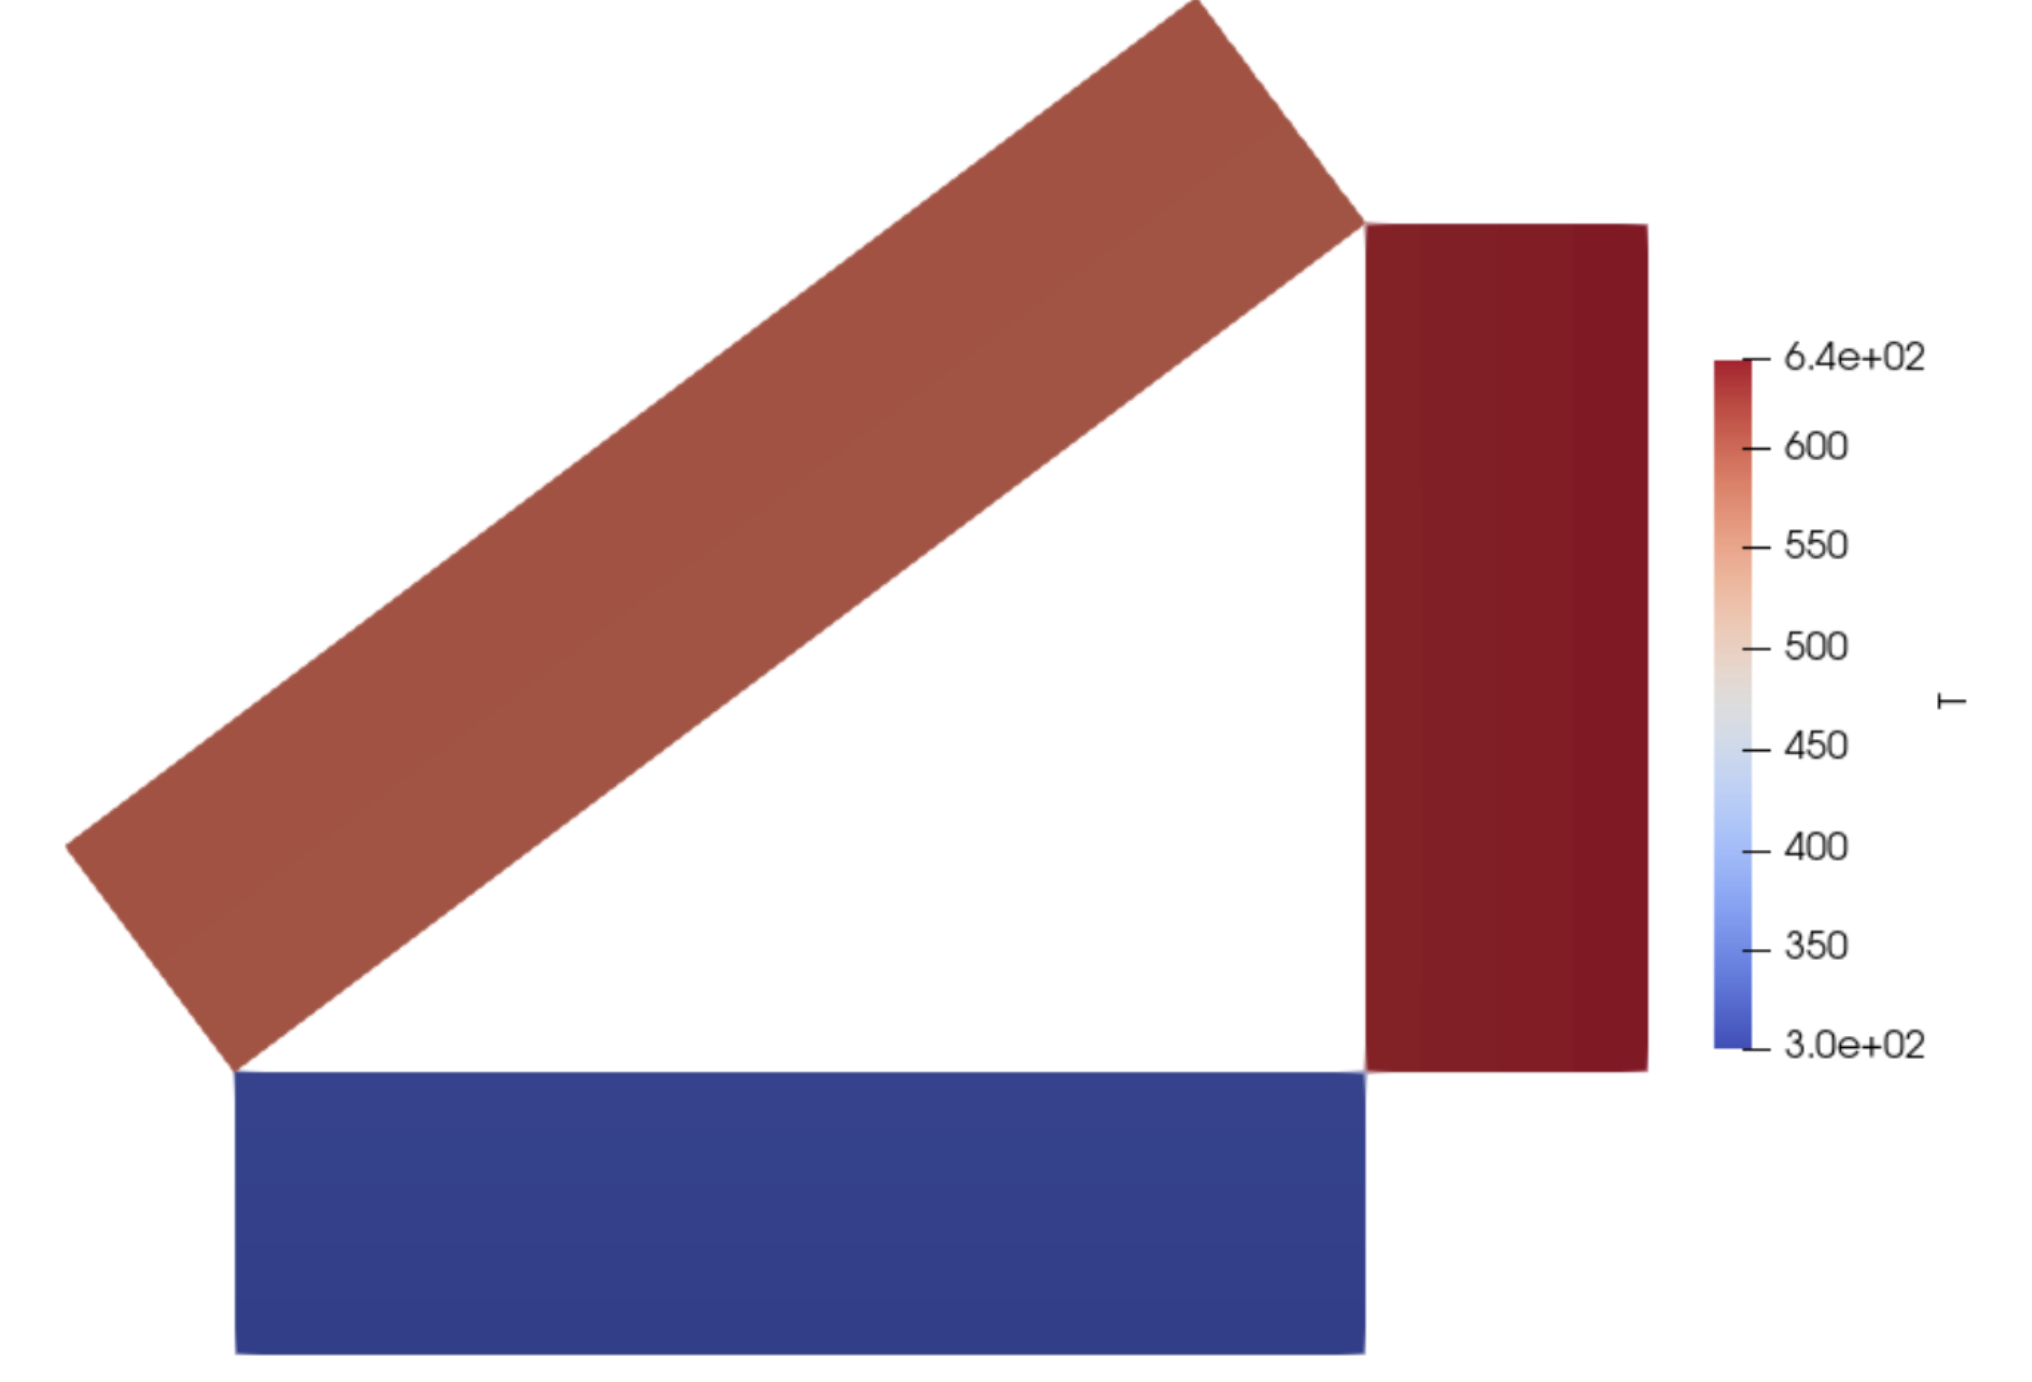
\includegraphics[width=0.45\textwidth]{CP114_img-view-factors-benchmark.png}
}
\caption{Solar masks and view factors computations}
\label{fig:solar-masks-vf}
\end{figure}




\subsubsection{Heat Transfer Modeling with Feel++ and Modelica}
\noindent
In the \textit{Urban Building Energy Model} (UBEM), heat transfer analysis predicts energy consumption, internal air temperatures, and overall building performance. We combine \textbf{Modelica} with \textbf{Feel++} to simulate urban building heat dynamics.

\paragraph{Modelica for Multizone Heat Transfer}
Modelica accommodates LOD-0 to LOD-1 building representations by generating Functional Mock-up Units (FMUs), which \texttt{Feel++} then loads. Input data (e.g., geometry, materials, occupancy) come from building metadata; missing details default to typical values based on construction era. Future work includes parametrized occupancy profiles tailored to building functions.

\paragraph{Finite Element Analysis with Feel++}
Feel++ augments Modelica's multizone models with detailed finite element analyses. Advanced techniques, such as reduced basis methods and parallel-in-time schemes, handle solar radiation and shading masks derived from geometric and dynamic conditions, improving the accuracy of solar heat gain calculations.

\paragraph{Integrated Approach and Challenges}
Monte Carlo or ray-tracing methods compute shading masks and view factors, which feed Modelica for precise thermal load predictions. To manage the large computational demands of city-scale simulations, our approach leverages CPU resources (and, prospectively, GPUs) alongside mesh partitioning. This ensures city-wide analyses remain efficient, integrating spatial data handling with the thermal modeling processes.
%By utilizing the combined strengths of Feel++ for detailed finite element analysis and Modelica for system-level energy simulation, the UBEM framework is a tool capable of %%addressing the complex dynamics of urban heat transfer and energy management.%

%Continuous Integration (CI) and Continuous Deployment (CD) are pivotal in developing and operating the Urban Building pilot. These practices enable efficient management of complex simulation software, ensuring seamless integration and deployment across various computational infrastructures.

%CI practices handle complex dependencies and computational requirements specific to urban building simulations. Key features include automated testing, code quality checks, and automated builds, ensuring the software remains robust and maintainable.

%CD practices are tailored to manage deployment complexities across different HPC environments using containerization through Apptainer. This approach facilitates consistent, reproducible deployments, optimizing performance and resource utilization.

\subsubsection{Input data}

To run a KUB simulation, several input files need to be generated.
We have several metadata files (in JSON format), mesh data files (in MSH format), and meteorological measurement files (in CSV format).
\Cref{tab:input-data-size-comparison} lists these files with their corresponding sizes for New York City, see~\cref{fig:city-ny-largescale}, and a duration of one year for the simulation.
In addition, we compared the size of the input data with the size of the zone.

\begin{table}[ht]
  \centering
  \caption{Size comparison of input data files for different geographical extents in New York City}
  \label{tab:input-data-size-comparison}
  \begin{tabularx}{.95\linewidth}{l *{3}{>{\RaggedLeft\arraybackslash}X}} 
      \toprule
      \textbf{Files} & \textbf{\text{4 $\times$ 4} \si{\kilo\meter\squared}} & \textbf{\text{10 $\times$ 10} \si{\kilo\meter\squared}} & \textbf{\text{20 $\times$ 20} \si{\kilo\meter\squared}} \\
      \midrule
      \texttt{geographicdata\_setup.json} & \SI{4.0}{\kilo\byte} & \SI{4.0}{\kilo\byte} & \SI{4.0}{\kilo\byte} \\ 
      \texttt{gis.json} & \SI{23}{\mega\byte} & \SI{117}{\mega\byte} & \SI{470}{\mega\byte} \\
      \texttt{mesh\_lod0.msh} & \SI{17}{\mega\byte} & \SI{112}{\mega\byte} & \SI{496}{\mega\byte} \\
      \texttt{mesh\_lod1.msh} & \SI{44}{\mega\byte} & \SI{240}{\mega\byte} & \SI{896}{\mega\byte} \\
      \texttt{weather-data-0.hourly-variables.csv} & \SI{384}{\kilo\byte} & \SI{384}{\kilo\byte} & \SI{384}{\kilo\byte} \\
      \texttt{weather-data.json} & \SI{4.0}{\kilo\byte} & \SI{4.0}{\kilo\byte} & \SI{4.0}{\kilo\byte} \\
      \bottomrule
  \end{tabularx}
  \end{table}

In the future, the input data is expected to grow even larger with the addition of new details such as roofs, building characteristics, vegetation (e.g., trees), and terrain information.
These enhancements will increase the complexity and accuracy of the simulation and the amount of data required to accurately model the urban environment.

\section{CI/CD Framework for the Urban Building Pilot}
\label{sec:cicd-framework}

The Urban Building (KUB) pilot builds on the Feel++ framework using a CI/CD process that relies on containerized environments to ensure consistent development and deployment.

\subsection{Standard CI/CD DevOps}
KUB adopts the Feel++ CI/CD framework, leveraging GitHub Actions and Docker to compile, test, and validate updates automatically. 
Docker images embedding Feel++ and its dependencies are stored on GitHub Container Registry, ensuring consistency across various environments. 
\cref{fig:feelpp-devops} shows the main CI/CD workflow, which integrates updates from multiple projects using features such as 
\begin{inparaenum}[\it (i)]
  \item Pull Requests for code verification, 
  \item a \verb+workflow_dispatch+ GUI for on-demand deployment or testing, and 
  \item Scheduled Runs for routine checks
\end{inparaenum}.

\begin{figure}
\centering
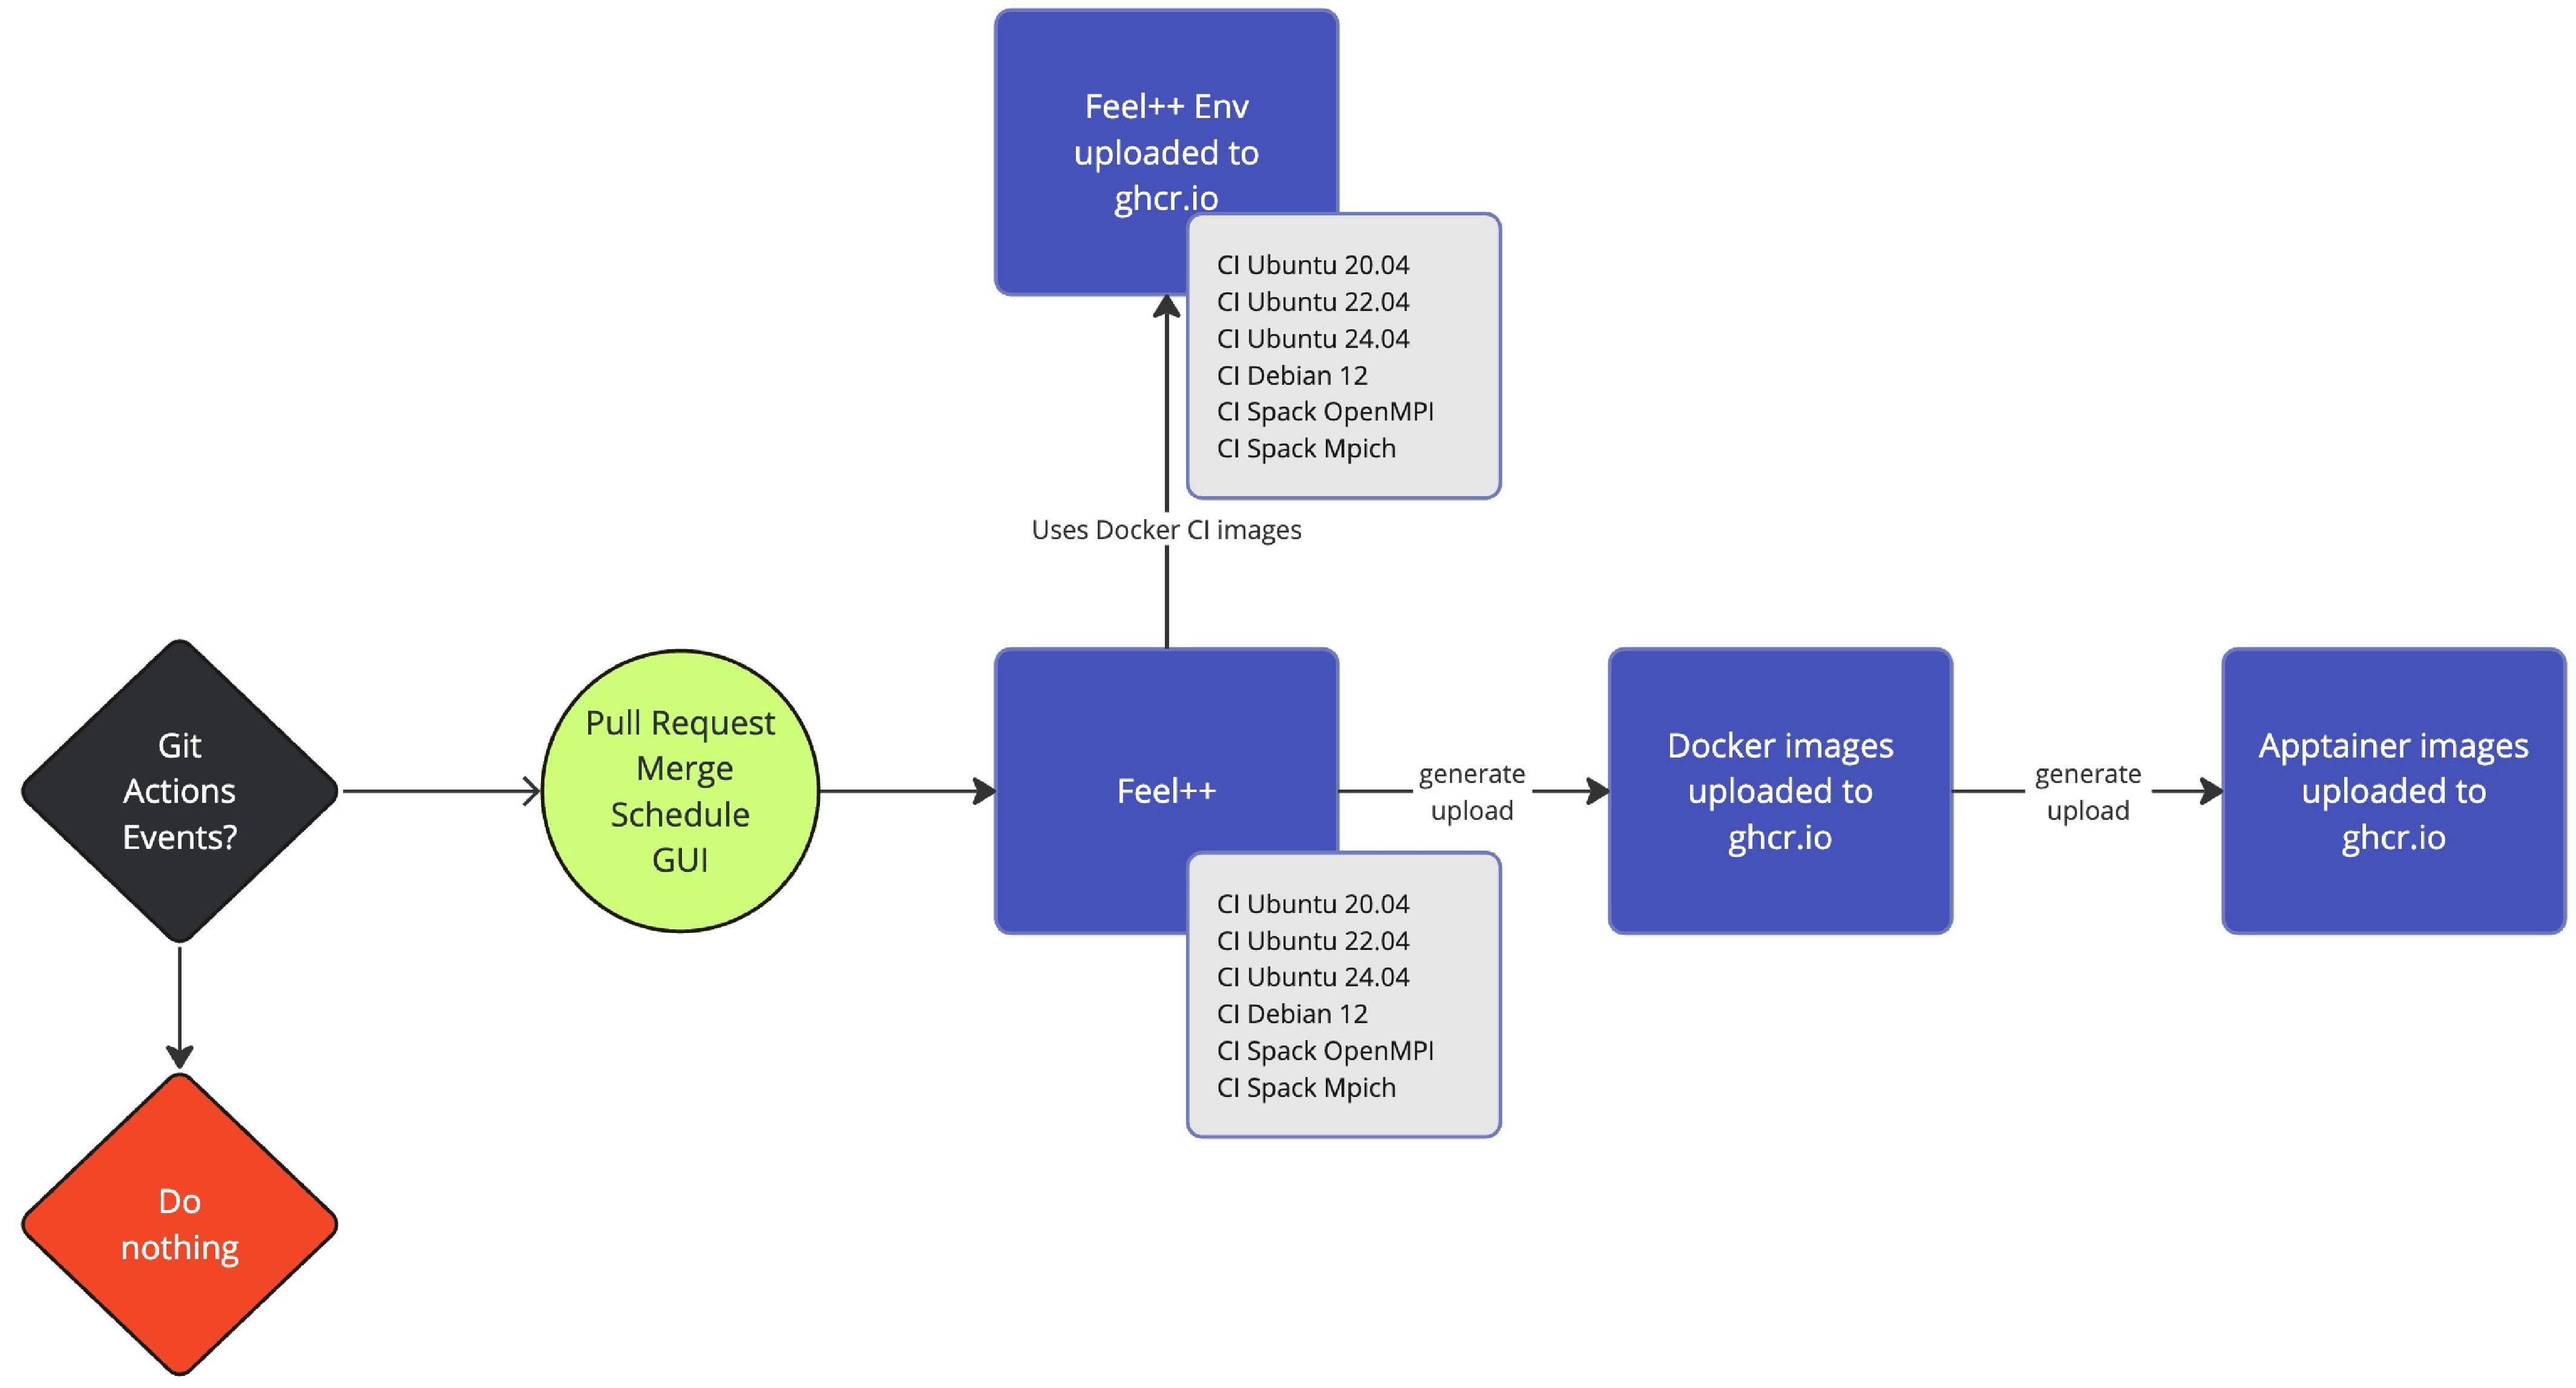
\includegraphics[width=\textwidth]{CP114_img-feelpp-devops.pdf}
\caption{CI/CD DevOps for Feel++}
\label{fig:feelpp-devops}
\end{figure}

\subsection{HPC DevOps (HPCOps)}
Feel++ CI/CD extends to HPCOps practices for large-scale simulations on systems such as LUMI, Karolina, and MeluXina. \cref{fig:feelpp-hpcops} illustrates this HPCOps workflow, which uses \begin{inparaenum}[\it (i)] \item ReFrame-HPC for systematic benchmarking~\cite{karakasis_reframe-hpcreframe_2024}, \item SLURM (REST API or scripts) for job scheduling~\cite{slurm_development_team_slurm_2024}, and \item Apptainer for secure container deployment in HPC settings~\cite{apptainer_contributors_apptainer_2024}\end{inparaenum}. Automated tests run on HPC nodes after basic checks succeed.

\begin{figure}
\centering
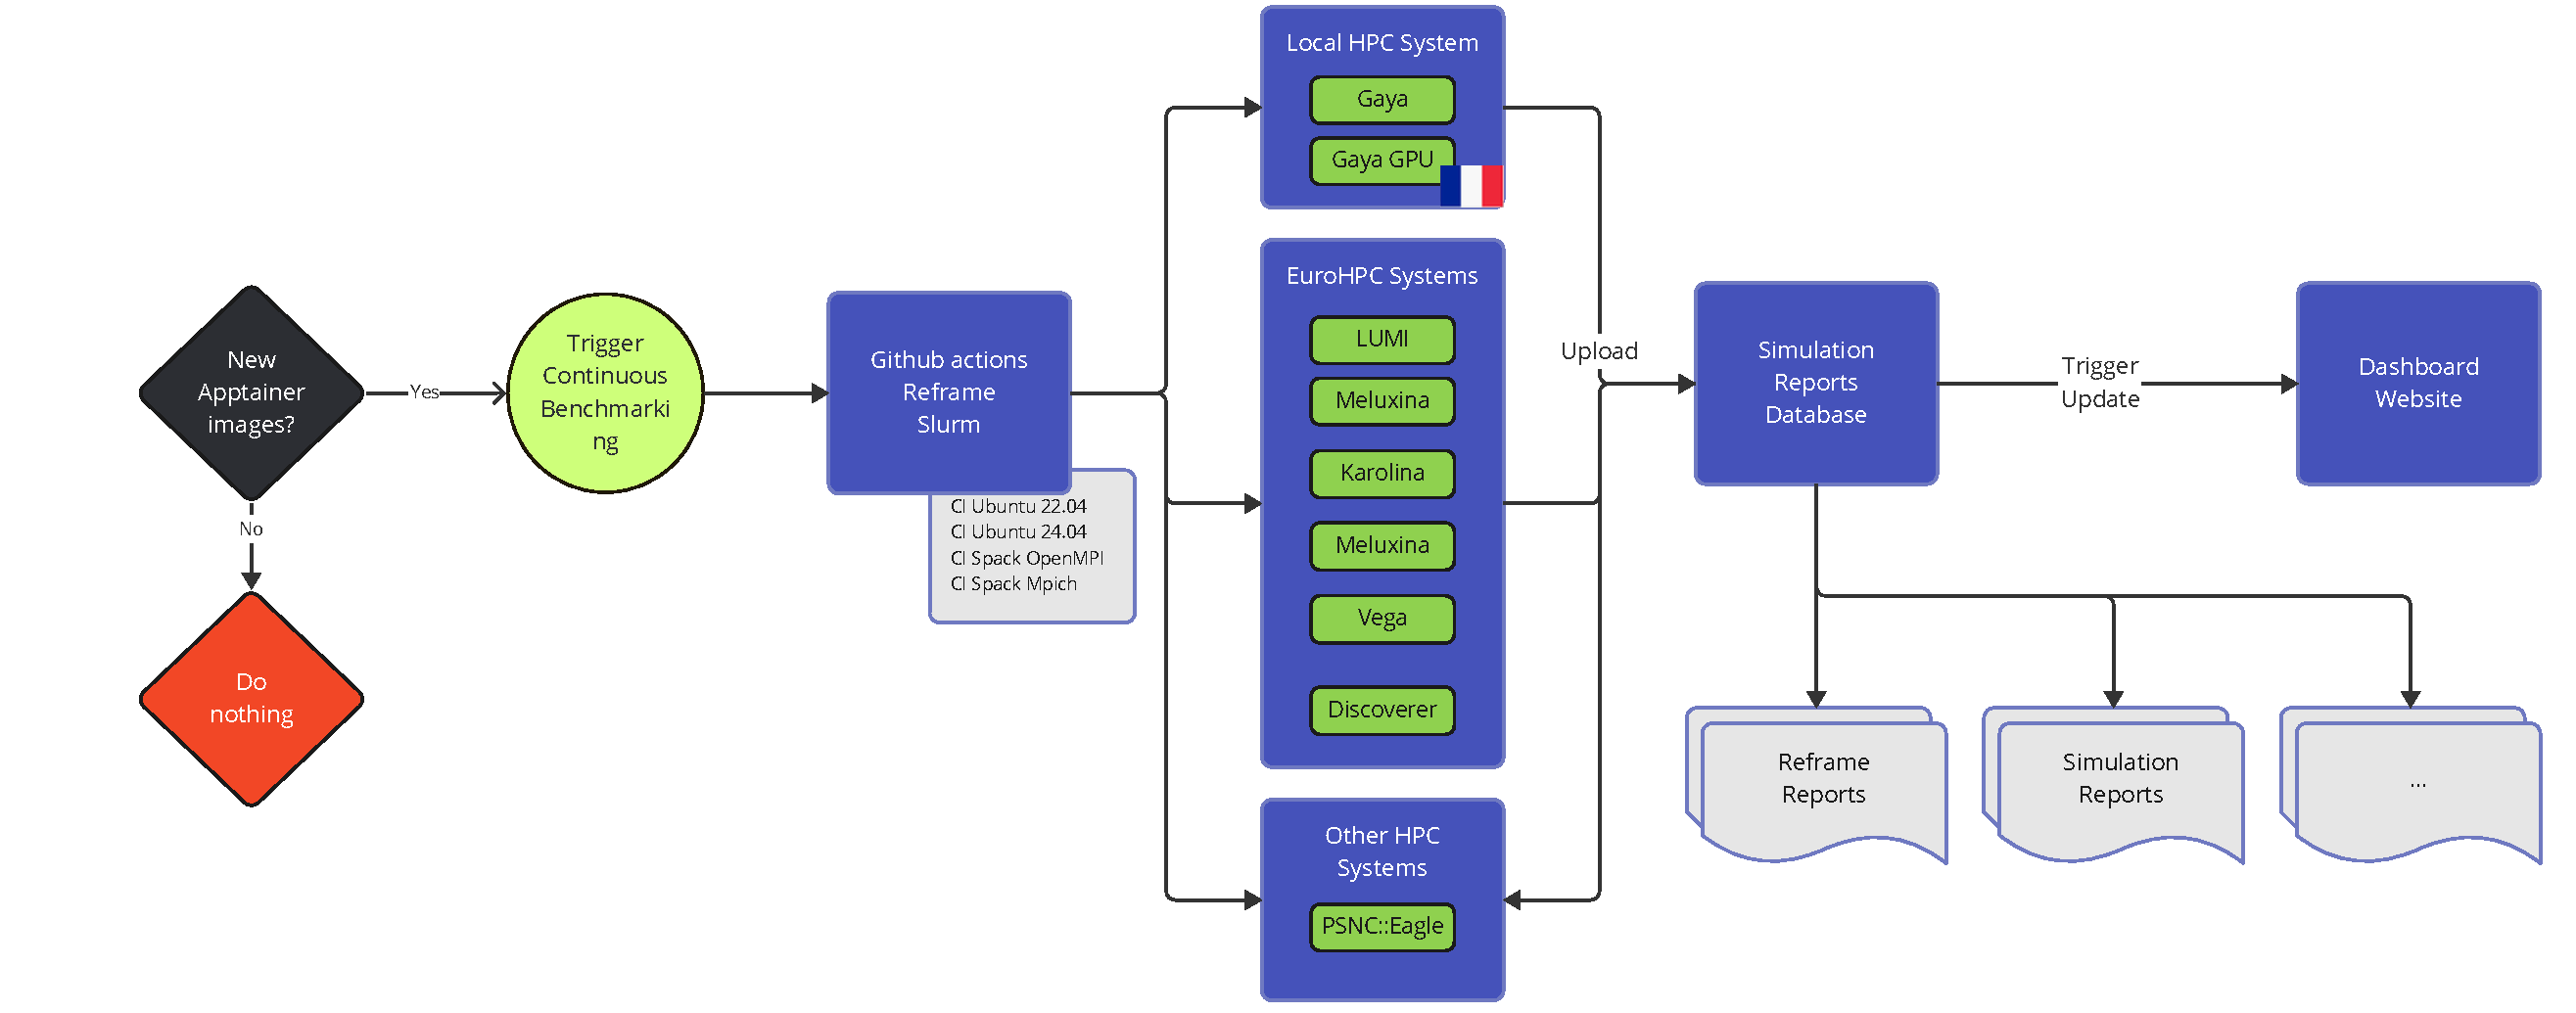
\includegraphics[width=\textwidth]{CP114_img-feelpp-hpcops.pdf}
\caption{CI/CD HPCOps for Feel++}
\label{fig:feelpp-hpcops}
\end{figure}

\Cref{fig:kub-devops} shows that KUB inherits the same DevOps steps, while \cref{fig:kub-hpcops} extends the HPCOps approach to handle more complex pre-/post-processing stages of the pilot.

\begin{wrapfigure}{R}{.7\linewidth}
\centering
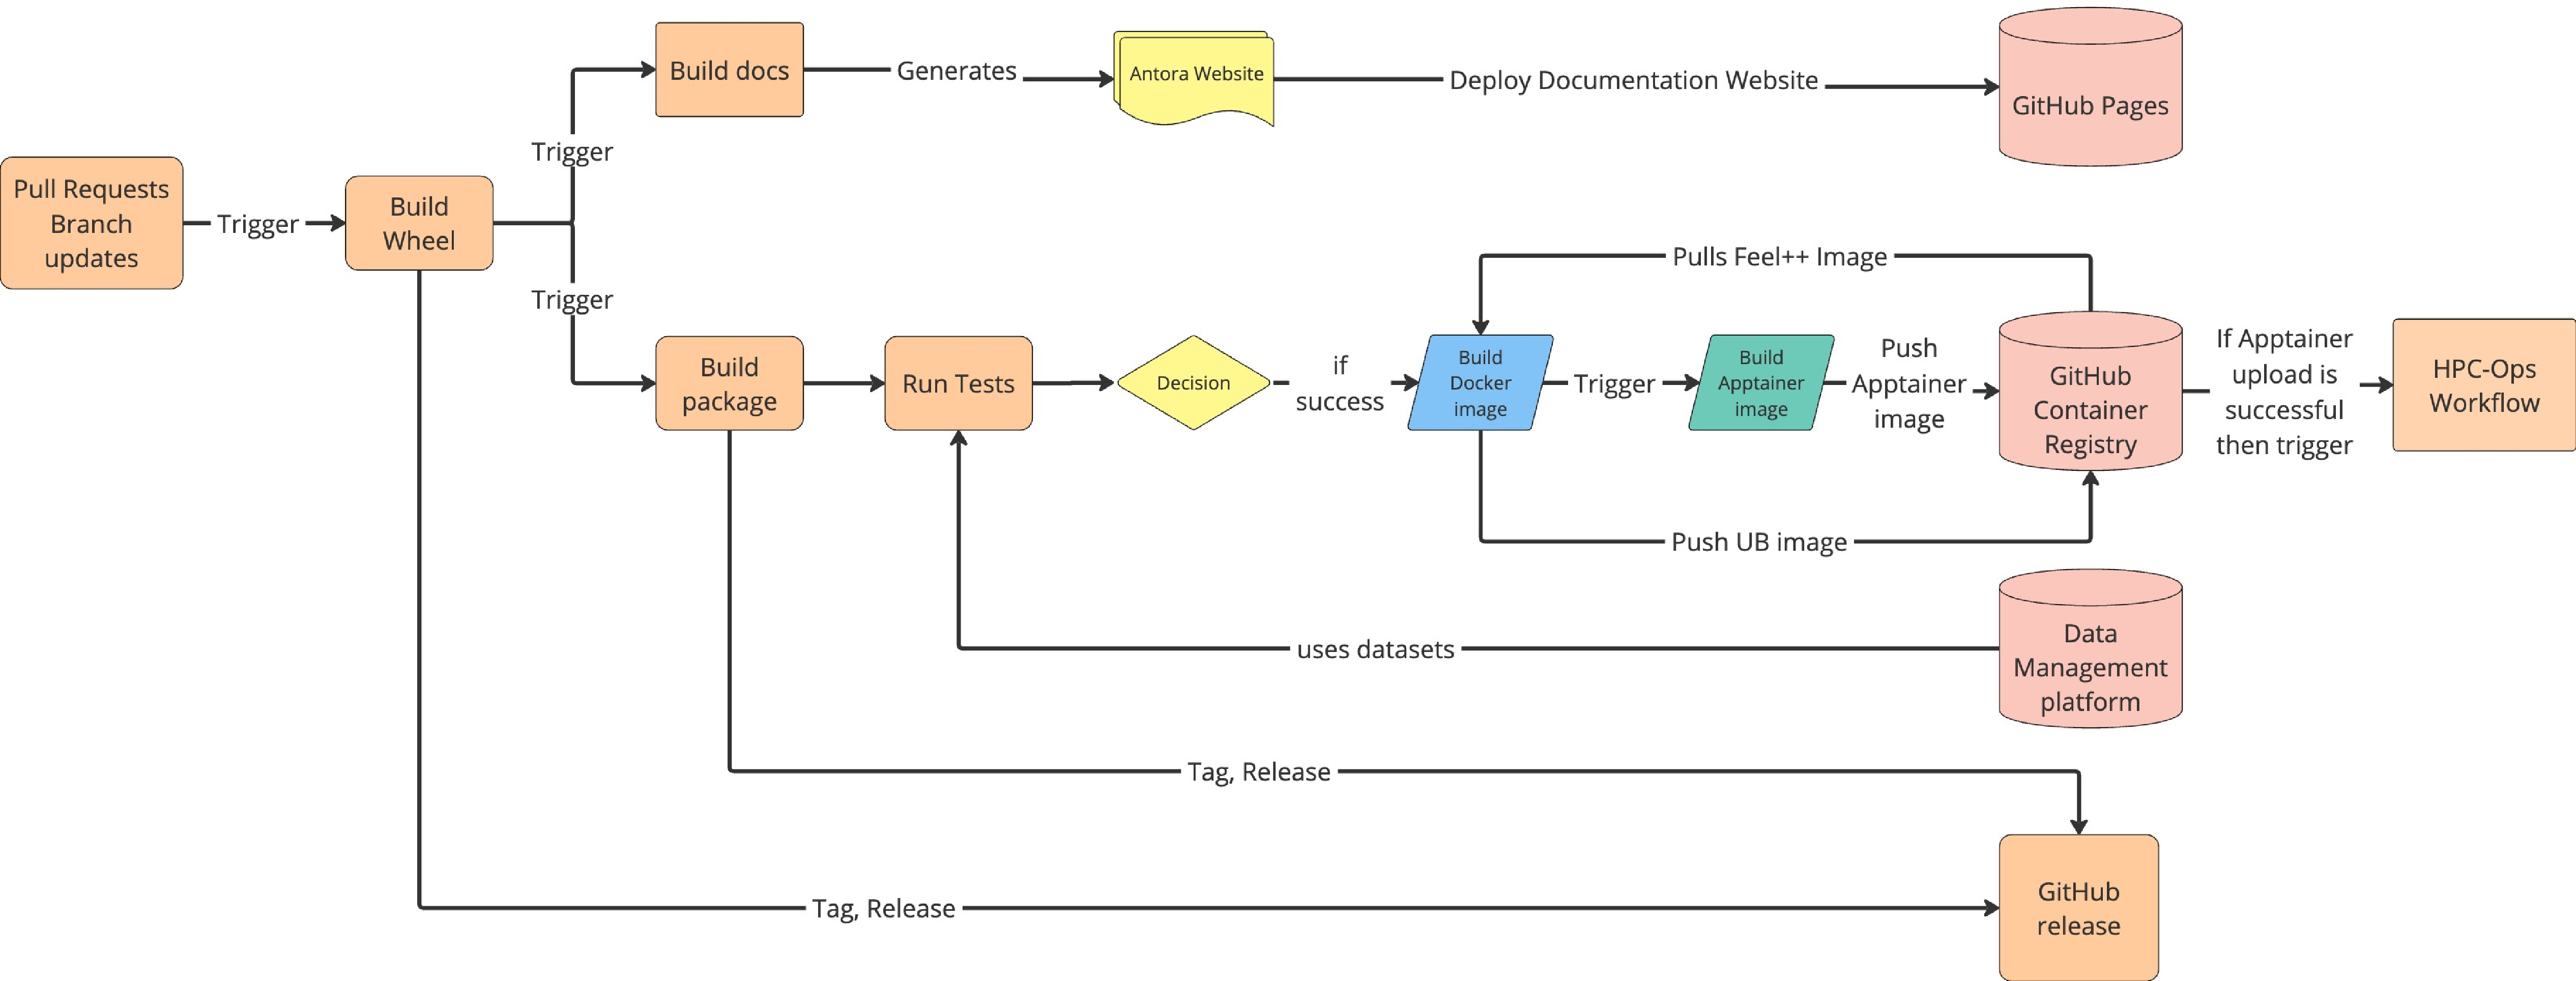
\includegraphics[width=\linewidth,page=1]{CP114_img-ub-devops-hpcops.pdf}
\caption{KUB standard DevOps}
\label{fig:kub-devops}
\end{wrapfigure}

\begin{figure}
\centering
\includegraphics[width=\linewidth,page=2]{CP114_img-ub-devops-hpcops.pdf}
\caption{Ktirio Urban Building HPCOps workflow}
\label{fig:kub-hpcops}
\end{figure}

\subsection{Benchmarking KUB}
\label{sec:benchmarking}
We next show benchmarking results~\cite{hidalgo2_d31_2024} for HPC performance on a $4 \mathrm{km}^2$ area in Strasbourg (about 17K buildings). \cref{fig:scalability} displays the speedup on Discoverer, Karolina, and MeluXina using our HPCOps pipeline (\cref{fig:kub-hpcops}): the simulation part scales linearly since buildings are decoupled, but total execution time does not. \cref{fig:execution-breakdown} reports the timing of pre-processing, simulation, and post-processing. As more nodes are used, post-processing (file I/O) becomes dominant and reduces overall scalability. In typical use, however, focusing on specific outputs diminishes that overhead.

\begin{wrapfigure}{R}{0.6\textwidth}
\centering
\begin{subfloat}[Scalability on EuroHPC systems from 1 to 32 nodes of 128 cores each]{
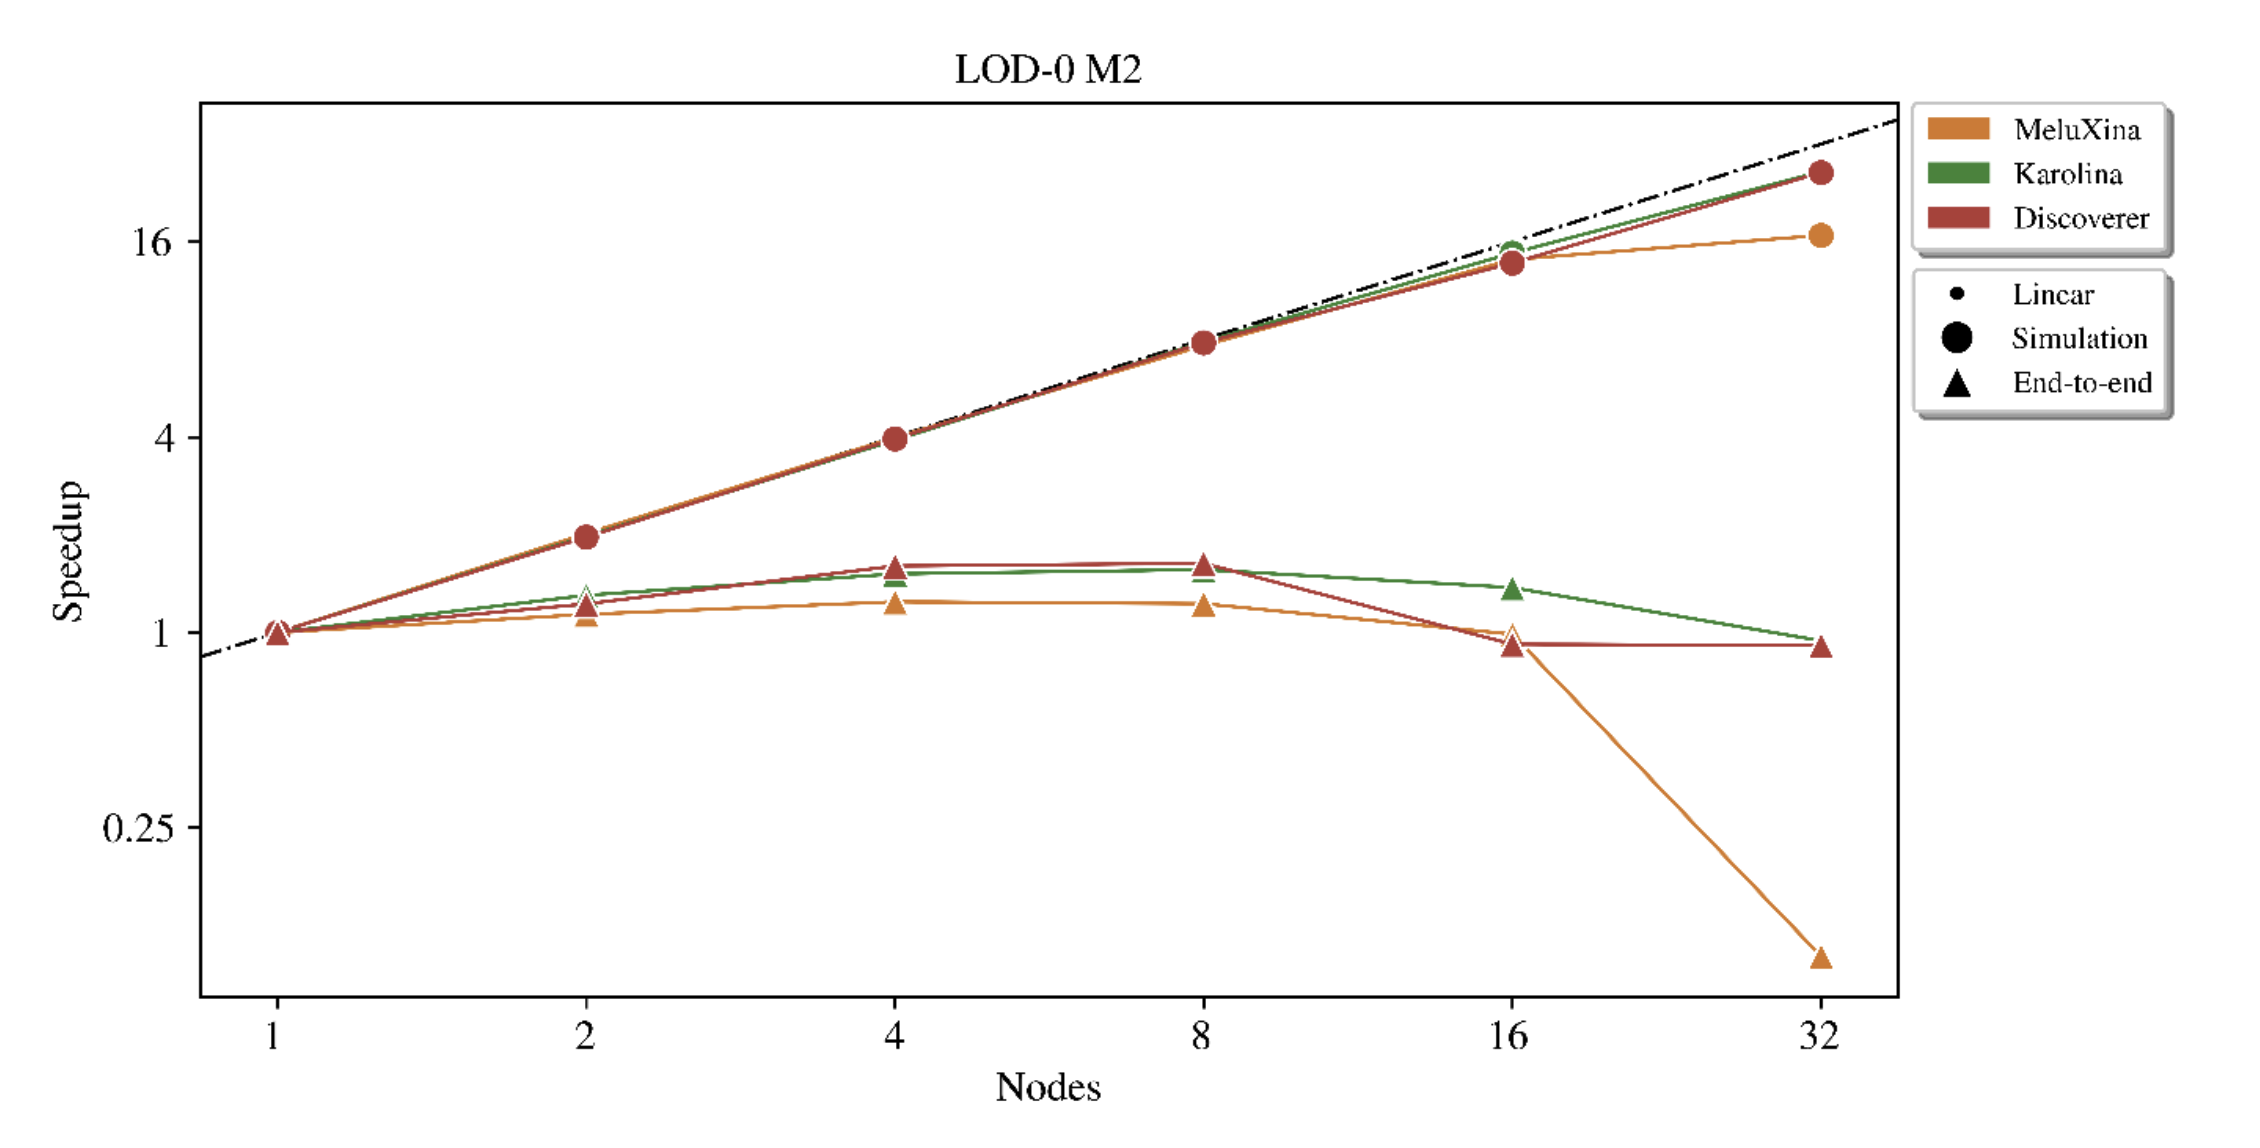
\includegraphics[width=0.9\linewidth]{CP114_img-kub-scalability.png}
\label{fig:scalability}
}\end{subfloat}
\
\begin{subfloat}[Execution breakdown on EuroHPC systems from 1 to 32 nodes of 128 cores each]{
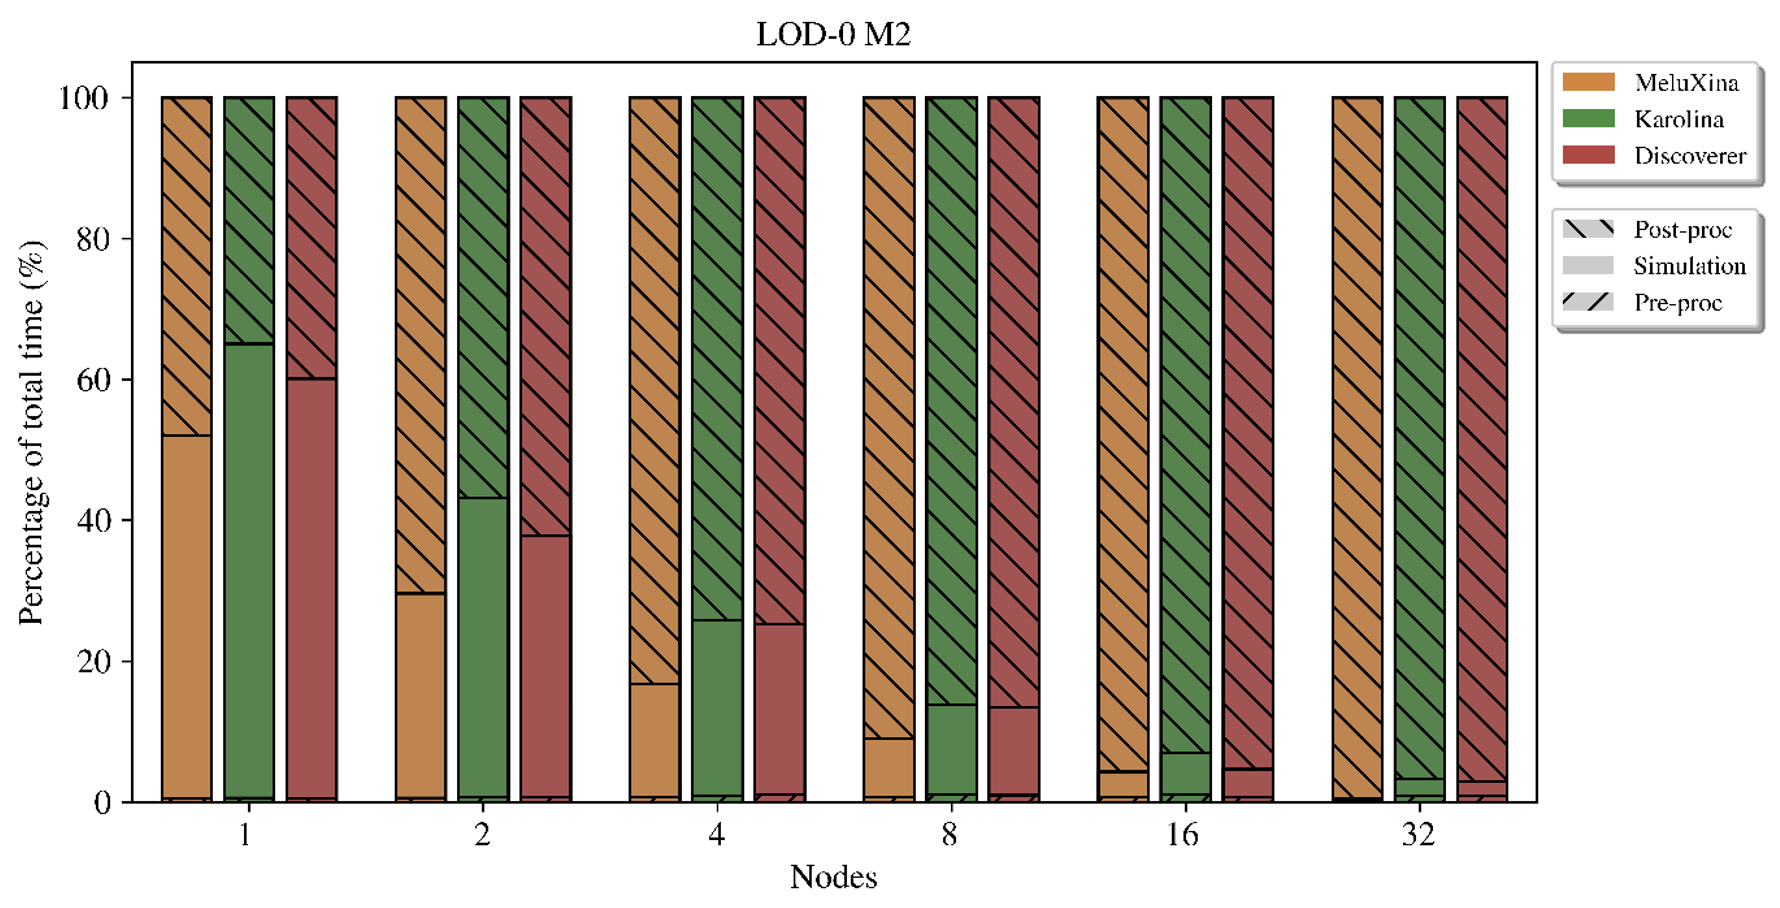
\includegraphics[width=0.9\linewidth]{CP114_img-kub-bencharkings-execution.png}
\label{fig:execution-breakdown}
}\end{subfloat}
\caption{Scalability and execution metrics for KUB on EuroHPC systems}
\label{fig:combined-metrics}
\end{wrapfigure}

Future improvements may include asynchronous writes or data caching. As models grow more complex (\cref{sec:heat-transfer-in-buildings}), the overall simulation time is expected to increase, reducing the relative impact of file operations.
\section{Conclusion}
\label{sec:conclusion}

We are developing the computational Ktirio Urban Building(KUB) framework: assembling this very compelling application encompasses challenges in mathematics --- scalable modeling and simulation, large-scale watertight robust mesh generation, advanced analysis including data simulation --- and computer science --- scalable framework, software architecture, modern development, testing and packaging environment including standard DevOps and now HPCOps.---
The overall programming, integration, delivery, and deployment environment is critical to develop such an application. To our knowledge, this is the first application that can be automatically benchmarked and executed on EuroHPC JU systems thanks to CI/CD or HPCOps. Moreover, the workflow from Feel++ to KUB provides a considerable gain in terms of development and testing time, automated as much as possible, and enabling researchers and developers to focus their work better.

Our next steps include \textit{(i)} enabling tasks-based parallelism using the C++ framework Specx, see~\cite{cardosi_specx_2022}; \textit{(ii)} improving the modeling and simulation components, including mesh generation, handling of vegetation and urban furniture, and enabling view factors as well as providing a variety of configurable building energy models; \textit{(iii)} enhanced parallel strategies particularly in terms of partitioning and improved large scale I/O; and of course \textit{(iv)} pursue our benchmarking activities on EuroHPC JU supercomputers.


\begin{credits}
\subsubsection{\ackname} Funded by the  European  Union. This work has received funding from the European High-Performance Computing Joint Undertaking (EuroHPC JU)  and  Poland, Germany,  Spain,  Hungary,  France, and Greece under grant agreement number 101093457. This  publication  expresses  the  opinions  of  the  authors  and  not  necessarily those of the EuroHPC JU and Associated Countries which are not responsible for any use of the information contained in this publication

Part of this work was also funded by \textit{(i)} the France 2030 NumPEx Exa-MA (ANR-22-EXNU-0002) project managed by the French National Research Agency (ANR), \textit{(ii)} AMIES, the french agency for interaction between mathematics and enterprises and \textit{(iii)} CNRS through its prematuration programme.

We acknowledge the EuroHPC Joint Undertaking for awarding this project access through  EuroHPC Development Access grants EHPC-DEV-2024D05-025 and EHPC-DEV-2023D08-047 to the EuroHPC JU supercomputers : \textit{(i)} Kumi, hosted by CSC (Finland) and the Lumi consortium, \textit{(ii)} MeluXina hosted by LuxProvide, Luxembourg, \textit{(iii)} Karolina hosted by IT4Innovations National Supercomputing Center, Czechia, \textit{(iv)} Discoverer hosted by Sofia Tech Park, Bulgaria, \textit{(v)} Vega hosted by IZUM, Slovenia, and \textit{(vi)} Leonardo hosted by CINECA, Italy.


Finally the authors would like to acknowledge the many fruitful discussions with our partners Luc Kern from Synapse Concept and Leopold Fischer from Cisco Meraki, our colleagues \textit{(i)} from Hidalgo2 ICCS Kostis Nikas, Aristomenis Theodoridis and Petros Anastasiadis for the discussions on Reframe and joining their EuroHPC access grant, \textit{(ii)} Hidalgo2 HLRS Sameer Haroon for the discussions on CI/CD, \textit{(iii)} Pierre Alliez from INRIA Titane and Andreas Fabri from Geometry Factory regarding the discussions on CGAL and using Polygon Repair, and finally \textit{(iv)} our former colleague Zohra Djatouti, now at Kipsum, which whom we initiated this endeavor.

% \subsubsection{\discintname}
% It is now necessary to declare any competing interests or to specifically
% state that the authors have no competing interests. Please place the
% statement with a bold run-in heading in small font size beneath the
% (optional) acknowledgments\footnote{If EquinOCS, our proceedings submission
% system, is used, then the disclaimer can be provided directly in the system.},
% for example: The authors have no competing interests to declare that are
% relevant to the content of this article. Or: Author A has received research
% grants from Company W. Author B has received a speaker honorarium from
% Company X and owns stock in Company Y. Author C is a member of committee Z.
\end{credits}


\section*{Nomenclature}

\begin{multicols}{2}
$\alpha$ : Absorption of a material.\hfill[-]\\
$\alpha_{conv}$=10 : Heat conductance of convection.\hfill[-]\\
$\beta$ : Angle of inclination of the wall to the horizontal.\hfill[-]\\
$\Delta T$ : Temperature difference.\hfill[K]\\
$\epsilon$ : Emissivity of the surface.\hfill[-]\\
$\phi_{air}$ : Air heat flow.\hfill[W]\\
$\phi_{net}$ : Radiative heat flow.\hfill[W]\\
$\phi_{solar}$ : Solar heat flow from short wavelength.\hfill[W]\\
$\phi_{wall}$ : Heat flow through a wall.\hfill[W]\\
$\sigma$ : Stefan-Boltzmann constant $5,67\cdot10^{-8}$.\hfill[W$\cdot m^{-2}\cdot K^{-4}$]\\
$albedo$ : Reflective properties of the material.\hfill[-]\\
$A_z$ : Azimuth of the surface.\hfill[-]\\
$A_{zs}$ : Azimuth of the sun.\hfill[-]\\
$C$ : Heat capacity of the zone.\hfill[W$\cdot K^{-1}$]\\
$d_{inhabitant}(timetable)$ : Density of inhabitants as a function of the timetable set for the building type.\hfill[-]\\
$E_{dir}$ : Direct solar heat flow.\hfill[W$\cdot m^{-2}$]\\
$E_{diff}$ : Diffuse solar heat flow.\hfill[W$\cdot m^{-2}$]\\
$E_{ref}$ : Reflected solar heat flow.\hfill[W$\cdot m^{-2}$]\\
$F_{dir}$ : Direct solar radiation.\hfill[W$\cdot m^{-2}$]\\
$F_{dir,Hz}$ : Direct solar radiation on a horizontal surface given by climate data.\hfill[W$\cdot m^{-2}$]\\
$F_{ij}$ : View factor between $surface_{(i)}$ and $surface_{(j)}$.\hfill[-]\\
$H_s$ : Angular height of the sun.\hfill[-]\\
$J$ : Radiosity of a surface.\hfill[W$\cdot m^{-2}$]\\
$Met$ : Metabolic rate.\hfill[W]\\
$0.34\cdot Q_v$ : Airflow as a fraction of the zone's volume per hour multiplied by the air volumetric heat capacity.\hfill[W$\cdot K^{-1}$]\\
$S$ : Surface area.\hfill[m$^2$]\\
$S_C$ : Shading coefficient $\in$ [0,1].\hfill[-]\\
$U_j$ : Conductance of a $wall_j$.\hfill[W$\cdot m^{-2}\cdot K^{-1}$]\\
$V_{air}$ : Wind speed.\hfill[m$\cdot s^{-1}$]
\end{multicols}

\bibliographystyle{splncs04}
\bibliography{CP114_references}

\end{document}
